\chapter{Analysis Strategy}%
\label{ch:strategy}
In the previous chapter the process of reconstruction and selection was
described. With the objects required for this analysis reconstructed and an
event selection in place an analysis strategy is formed in order to maximise the
signal strength of the VH(bb) process and yield a robust result that is well
understood in terms of modelling and systematic errors. In this chapter that
strategy will be detailed, first the categorisation into analysis regions will
be defined, next the multi-variate algorithm that is used to generate some of
the distributions entering into the profile-likelihood fit will be explained.
Plots of the data versus Monte-Carlo prediction will then be shown in order to
build a picture of the pre-fit status of the agreement. Finally a series of
cross-checks which are used to validate the methods of the analysis will be
explained.

The author's contributions include studying the behaviour of the
profile-likelihood fit with the inclusion of these regions, which are new in
this round of the analysis and making comparisons between the 80~\invfb and
140~\invfb datasets). Contributions also include the training of the
multi-variate classification algorithm with the inclusion of new input variables
with respect to the previous version of the algorithm.

\section{Categorisation into Analysis Regions}
\label{sec:ana-regions}

Events which pass the selection detailed in table~\ref{tab:event-selection} are
categorised into several regions for analysis. Firstly they are split into what
are known as medium ($75 - 150 \GeV$), high ($150 - 250 \GeV$) and extreme ($ >
250 \GeV$) $p_T^{V}$. Events are further categorised by jet multiplicity, all
jets are required by the selection to have at least two jets, categories are
defined for events with exactly two, or exactly three jets. In the 2--lepton
channel there is a requirement of three or more jets but when referring to all
three channels at once categorisation is referred to as simply 3-jet or 2-jet.

Furthermore events are categorised into a so-called signal region which is
straddled either side by two control regions. This categorisation is achieved
via continuous cuts defined in the $\Delta R(b, \bar{b})$~---~$p_T^{V}$ plane,
they are chosen to maximise the signal purity in the signal region and are shown
for the 1--lepton channel in figure~\ref{fig:drbb-crs}.
\begin{figure}[h]
  \centering
  \begin{tabular}{cc}
    \subfloat[]{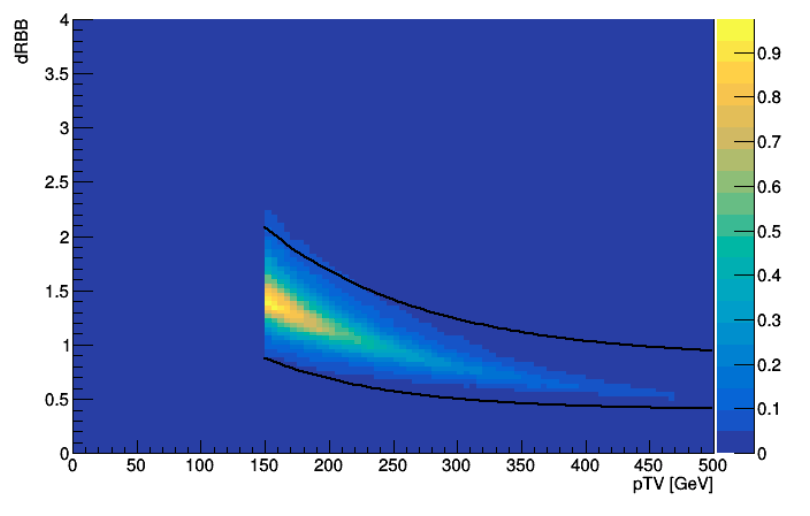
\includegraphics[width=0.505\linewidth]{1lep_qqWH_2tag_2jet.png}}
    \subfloat[]{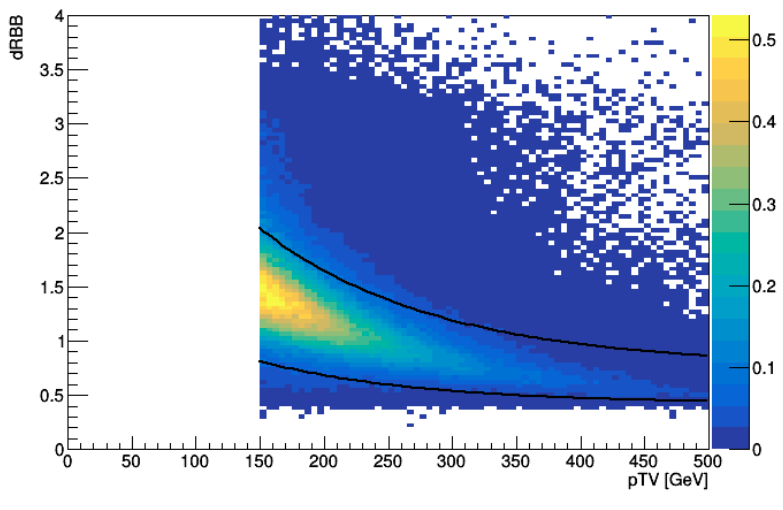
\includegraphics[width=0.49\linewidth]{1lep_qqWH_2tag_3jet.png}}\\
  \end{tabular}
  \caption{Signal distribution of $\Delta R$ between the two selected jets as
    function of $p_{T}^{V}$ in the 1-lepton channel are shown in the 2-tag 2-jet
    (a) and 2-tag 3-jet (b) categories. The black lines demonstrate the upper
    and lower continuous cuts used to categorise the events into the signal and
    control regions}
  \label{fig:drbb-crs}
\end{figure}
The control regions either side of the signal region are known as the
high-$\Delta R(b, \bar{b})$ and low-$\Delta R(b, \bar{b})$ regions, shortened to
CRHigh and CRLow respectively.

A 3D representation of the regions defined when combining these three
categorisations can be seen in figure~\ref{fig:analysis-categories}.
\begin{figure}[ht]
  \centering
  \begin{tikzpicture}[every node/.style={minimum size=1cm},on grid]
\begin{scope}[every node/.append style={yslant=-0.5},yslant=-0.5]
  \path (0,0) rectangle +(3,3);
  \node at (0.5,2.5) {};
  \node at (1.5,2.5) {};
  \node at (2.5,2.5) {};
  \node at (0.5,1.5) {};
  \node at (1.5,1.5) {};
  \node at (2.5,1.5) {};
  \node at (0.5,0.5) {};
  \node at (1.5,0.5) {};
  \node at (2.5,0.5) {};
  \draw (0,0) grid (3,3);
\end{scope}
\begin{scope}[every node/.append style={yslant=0.5},yslant=0.5]
  \path (3,-3) rectangle +(3,3);
  \node at (3.5,-0.5) {};
  \node at (4.5,-0.5) {};
  \node at (5.5,-0.5) {};
  \node at (3.5,-1.5) {};
  \node at (4.5,-1.5) {};
  \node at (5.5,-1.5) {};
  \node at (3.5,-2.5) {};
  \node at (4.5,-2.5) {};
  \node at (5.5,-2.5) {};
  \draw (3,-3) grid (6,0);
\end{scope}
\begin{scope}[every node/.append style={
    yslant=0.5,xslant=-1},yslant=0.5,xslant=-1
  ]
  \path (6,3) rectangle +(-3,-3);
  \node at (3.5,2.5) {};
  \node at (3.5,1.5) {};
  \node at (3.5,0.5) {};
  \node at (4.5,2.5) {};
  \node at (4.5,1.5) {};
  \node at (4.5,0.5) {};
  \node at (5.5,2.5) {};
  \node at (5.5,1.5) {};
  \node at (5.5,0.5) {};
  \draw (3,0) grid (6,3);
\end{scope}
\end{tikzpicture}
\caption{A graphic representation of the analysis categories.}
\label{fig:analysis-categories}
\end{figure}

Note that not all regions of the cube are populated with events in every channel, the medium
$p_T^V$ region is only filled for the 2--lepton channel.

\subsection{Top \texorpdfstring{$e \mu$}{e mu} control region}%
\label{sec:topemucr}

One more region exists only in the 2--lepton channel, it is obtained by inverting the
requirement of two same flavour leptons, requiring two opposite flavour leptons
instead, and keeping all other selection criteria the same. This region contains
almost all $t\bar{t}$ and single top processes (whose Feynman diagrams belong to
the same sum) matching very closely the number of expected events of each of
these backgrounds in the 2--lepton channel. This region is therefore called the
top $e \mu$ control region. The data from this control region can be used as a
prediction for the number of top process events in the 2--lepton channel once
multiplied by a scale factor which accounts for differences in normalisation.
Since data are used as the prediction for these events modelling of shape or
migration between control regions becomes unnecessary.

Plots of top e-mu control region

\section{Composition of Analysis Regions}

This section will detail the composition of each analysis region in terms of
background and signal processes. For all regions the signal process is
$VH~\rightarrow~b\bar{b}$, the prediction for which comes from events generated
using \textsc{Powheg MiNLO}~+~\textsc{Pythia~8} for quark initiated processes
and \textsc{Powheg}~+~\textsc{Pythia~8} for gluon initiated processes as can be
seen in table~\ref{tab:sigMC}.
 
\begin{table}[tbph]
\centering
\resizebox{\textwidth}{!}{
  \begin{tabular}{llrS[table-format=3.2]S[table-format=3.2]S[table-format=3.2]}
    \toprule
    {\bfseries Process} & {\bfseries Generator} & \bfseries{$\bm{\sigma \times BR}$ [pb]} & \multicolumn{3}{c}{{\bfseries $\bm{N_{\text{events}}}$ in millions}}\\
                        &&&\bfseries{mc16a}&\bfseries{mc16d}&\bfseries{mc16e}\\
    \midrule

    $qq \to ZH \to \nu\nu b\bar{b}$ & \textsc{Powheg MiNLO} + \textsc{Pythia 8 } (NNPDF3)& $153.05\times0.582$ & 2  & 2  & 3.3  \\
    $qq \to WH \to l^+\nu b\bar{b}$ & \textsc{Powheg MiNLO} + \textsc{Pythia 8 } (NNPDF3)& $282.78\times0.582$ & 4  & 4  & 6.6  \\
    $qq \to WH \to l^-\nu b\bar{b}$ & \textsc{Powheg MiNLO} + \textsc{Pythia 8 } (NNPDF3) & $179.49\times0.582$ & 2  & 2  & 3.3  \\
    $qq \to ZH \to ll b\bar{b}$ & \textsc{Powheg MiNLO} + \textsc{Pythia 8 } (NNPDF3)& $77.04\times0.582$ & 3  & 3  & 5  \\
    $gg \to ZH \to \nu\nu b\bar{b}$ & \textsc{Powheg} + \textsc{Pythia 8}  (NNPDF3) & $24.57\times0.582$ & 0.5  & 0.5  & 0.5  \\
    $gg \to ZH \to l^{-}l^{+} b\bar{b}$ & \textsc{Powheg} + \textsc{Pythia 8} (NNPDF3) & $12.42\times0.582$ & 0.75  & 0.75  & 0.75  \\
\bottomrule
\end{tabular}
}
\caption{Monte Carlo samples used for the signal processes and the cross section
  and branching ratio (BR) used to normalise the different processes at
  $\sqrt{s}=13$~TeV. Branching ratios correspond to the $H\rightarrow b\bar{b}$
  decay while $V$ branching ratio are still included in the cross-section. This
  was made to make easier the comparison with the reference tables computed
  including $V$ decays in~\cite{twikiCrossSections}. $l$ corresponds to all $e$,
  $\mu$ and $\tau$ leptons together.}
\label{tab:sigMC}
\end{table}


The 0--lepton channel contains the  Z+ jets, W + jets, top quark and diboson
backgrounds. The Z + jets background dominates the mixture in the 2-jet category
across signal and control regions. In the 3-jet category the top-quark processes
dominate apart from in the low $\Delta R(b, \bar{b})$ region. There is very
little signal contamination in the control regions. As can be seen in
table~\ref{tab:bkgMC} V + jets events are generated using \textsc{Sherpa~2.2.1},
top quark events are generated using \textsc{Powheg}~+~\textsc{Pythia~8} and
diboson events are generated also using \textsc{Sherpa~2.2.1}, this is true for
these backgrounds across all channels where a Monte-Carlo prediction is used.

\begin{table}[tbph]
\centering
\resizebox{\textwidth}{!}{
  \begin{tabular}{lllrrrr}
    \toprule
    \multicolumn{2}{l}{{\bfseries Process}} & {\bfseries Generator} & \bfseries{$\bm{\sigma \times BR}$ [pb]} & \bfseries{$\bm{N_{\text{events}}}$ (mc16a)} & \bfseries{$\bm{N_{\text{events}}}$ (mc16d)} & \bfseries{$\bm{N_{\text{events}}}$ (mc16e)}\\
    \midrule
    \multicolumn{2}{l}{\bfseries{Vector boson + jets}} & & & & & \\
    \multicolumn{2}{l}{$Z \to \nu\nu$} & \textsc{Sherpa} $2.2.1$ & $56280\times0.200$ & 150M & 160M & 140M \\
    \multicolumn{2}{l}{$W \to \ell\nu$} & \textsc{Sherpa} $2.2.1$ & $183600\times0.325$ & 340M & 400M & 540M \\
    \multicolumn{2}{l}{$Z/\gamma^{*} \to \ell\ell$} & \textsc{Sherpa} $2.2.1$ & $61940\times0.101$ & 120M & 160M & 210M \\
    \multicolumn{2}{l}{\bfseries{Top-quark}} & & & & & \\
    $t\bar{t}$ & non-full-had (plus MET/pTW extensions) & \textsc{Powheg} + \textsc{Pythia 8} & $831.76\times0.543$ & 120M(55M) & 150M(55M) & 200M(61M) \\
                                            & di-leptonic & \textsc{Powheg} + \textsc{Pythia 8} & $831.76\times0.105$ & $-$ & 45M & 100M \\
    Single-top & $s$~-~channel (leptonic-top) & \textsc{Powheg} + \textsc{Pythia 8} & $10.32\times0.325$ & 4M & 5M & 7M \\
                                            & $t$~-~channel (leptonic-top) & \textsc{Powheg} + \textsc{Pythia 8} & $216.96\times0.325$ & 10M & 12M & 17M \\
                                            & $Wt$~-~channel (plus di-lepton extension)& \textsc{Powheg} + \textsc{Pythia 8} & $71.7\times1$ & 20M & 24M(24M) & 33M(33M) \\
    \multicolumn{2}{l}{\bfseries{Diboson}} & & & & & \\
    $qq\rightarrow WW$ & $\rightarrow qqlv$ & \textsc{Sherpa 2.2.1} & $112.6\times0.439$ & 14M & 50M & 24M \\
    $qq\rightarrow WZ$ & $\rightarrow lvqq$ (with $Z\rightarrow b\bar{b}$ extension) & \textsc{Sherpa 2.2.1} & $50.3\times0.227$ & 7M(6M) & 36M(7M) & 12M(10M) \\
                                            & $\rightarrow qqvv$ & \textsc{Sherpa 2.2.1} & $50.3\times0.135$ & 6M & 6M & 10M \\
                                            & $\rightarrow qqll$ & \textsc{Sherpa 2.2.1} & $50.3\times0.0683$ & 5M & 27M & 9M \\
    $qq\rightarrow ZZ$ & $\rightarrow qqll$ (with $Z\rightarrow b\bar{b}$ extension) & \textsc{Sherpa 2.2.1} & $15.57\times0.140$ & 5M(5M)  & 5M(6M) & 9M(4M) \\
                                            & $\rightarrow qqvv$ (with $Z\rightarrow b\bar{b}$ extension) & \textsc{Sherpa 2.2.1} & $15.57\times0.280$ & 5M(5M)  & 5M(6M) & 9M(8M) \\
    \multicolumn{2}{l}{$gg\rightarrow WW \rightarrow qqlv$} & \textsc{Sherpa 2.2.2} & $4.8\times0.439$ & 0.8M & 0.9M & 1.1M \\
    \multicolumn{2}{l}{$gg\rightarrow ZZ \rightarrow qqll$ or $qqvv$} & \textsc{Sherpa 2.2.2} & $1.57\times0.420$ & 4M & 6M & 8M \\
    \bottomrule
  \end{tabular}
}
\caption{Monte Carlo samples used for the background processes and the cross
  section times branching ratio (BR) used to normalise the different processes
  at $\sqrt{s}=13$ TeV. The last column shows the number of simulated events for
  the {mc16a+d+e} production. Branching ratios correspond to the decays shown.
  In this table $\ell$ is inclusive of $e$, $\mu$, $\tau$ leptons. For
  $Z/\gamma^{*} \to \ell\ell$ events the requirement of $m_{\ell\ell}>40$~GeV
  was imposed.
%For the samples $WZ$ and $ZZ$ the number in brackets shows the number of additional events generated with the decay $Z \rightarrow b\bar{b}$.
}
\label{tbl:bkgMC}
\end{table}


The 1--lepton channel contains the W + jets, Z+ jets, top quark, diboson and multijet
backgrounds where multijet is the name given to backgrounds arising from QCD
processes. The channel is dominated by a mixture of W + jets and top quark
processes, the high $\Delta R(b, \bar{b})$ control region has a higher purity of
top quark processes whereas the low $\Delta R(b, \bar{b})$ control region has a
high purity of W + jets background. Contribution from multijet and Z + jets is
small across all regions, and similarly to in the 0--lepton channel the diboson
background is almost all contained in the signal region.

The 2--lepton channel contains the Z + jets, top quark and diboson backgrounds.
The Z + jets background dominates across all regions particularly in both
$\Delta R(b, \bar{b})$ control regions. Predictions for the top quark processes
are taken from the top $e \mu$ control region described in
section~\ref{sec:topemucr}. Given that these predictions come from data, the
importance of a good understanding of the remaining large background, Z + jets,
is crucial to the performance of the analysis.

\section{Multi-variate Event Classification}%
\label{sec:mva}

The signal regions in all channels enter into the profile-likelihood fit as
distributions generated by a multi-variate analysis. The multi-variate algorithm
used to generate this distribution is a BDT trained to separate
$VH~\rightarrow~b\bar{b}$ from events coming from any other source. Although in
the profile-likelihood fit only the signal region is input as a distribution of
BDT scores, the BDT itself is trained on the combination of all $\Delta R(b,
\bar{b})$ regions and takes place before the categorisation into ranges of
$p_T^V$. Apart from this all of the analysis selection criteria defined in
section~\ref{sec:selection} are applied before training. Training is carried out
separately for each lepton channel and jet multiplicity, a single split at
$150~\GeV$ is used in the 2--lepton channel resulting in eight separate regions
for training as in table~\ref{tab:training-regions}.
\begin{table}[h!tbp]
  \setlength{\extrarowheight}{2pt} 
  \centering
  \resizebox{\textwidth}{!}{
    \begin{tabular}{l l l l l}
      \toprule
      & \multicolumn{2}{l}{\bfseries $\bm{75}$~\GeV$\bm{ < p_{\text{T}}^V < 150}$~\GeV} & \multicolumn{2}{l}{\bfseries $\bm{p_{\text{T}}^V > 250}$~\GeV} \\
      {\bfseries Channel} & {\bfseries $\bm{2}$--jets} & {\bfseries $\bm{3}$--jets} & {\bfseries $\bm{2}$--jets} & {\bfseries $\bm{3}$--jets} \\
      \midrule
      $0$--lepton & $-$ & $-$ & $\checkmark$ & $\checkmark$ \\
      $1$--lepton & $-$ & $-$ & $\checkmark$ & $\checkmark$ \\
      $2$--lepton & $\checkmark$ & $\checkmark$ & $\checkmark$ & $\checkmark$ \\
      \bottomrule
    \end{tabular}
  }
\caption{Event categories on which the analysis BDT is trained, each box with a
  $\checkmark$ in represents a separate training.}
\label{tab:training-regions}
\end{table}
Training regions do not match the signal regions in terms of selection in order
to ensure that the training is as robust as possible to statistical
fluctuations. In tests it has been shown that there is significant evidence of
over-training when training is performed on the signal region (see appendix~\ref{app:over-training}).


Table~\ref{tab:MVAinputs} shows which variables are used as inputs to algorithm
in each analysis channel. Inputs are carefully chosen in order to maximise the
performance of the algorithm. 

and table~\ref{tab:BDTSetup} shows the choice of
hyper-parameters for the algorithm as described in \textsc{tmva}~\cite{TMVA} the
toolkit for multi-variate analysis which is built into
\textsc{ROOT}~\cite{ROOT}, and was used for training this algorithm.
\begin{table}[htbp]
\begin{center}
  \begin{tabular}{lllll}
    \toprule
    {\bfseries Variable} & {\bfseries Name} & {\bfseries 0-lepton} & {\bfseries 1-lepton} & {\bfseries 2-lepton} \\
    \midrule
    $m_{jj}$ & mBB & $\checkmark$ & $\checkmark$ & $\checkmark$ \\
    $\Delta R(jet_{1}, jet_{2})$ & dRBB & $\checkmark$ & $\checkmark$ & $\checkmark$ \\
    $p_{T}^{\text{jet1}}$ & pTB1 & $\checkmark$ & $\checkmark$ & $\checkmark$ \\
    $p_{T}^{\text{jet2}}$ & pTB2 & $\checkmark$ & $\checkmark$ & $\checkmark$ \\
    $p_{T}^{V}$ & pTV & \checkmark & $\checkmark$ & $\checkmark$ \\
    $\Delta \phi(V, H)$ & dPhiVBB & $\checkmark$ & $\checkmark$ & $\checkmark$ \\
    binned MV2c10(jet$_{1}$) & bin\_MV2c10B1 & $\checkmark$ & $\checkmark$ &  \\
    binned MV2c10(jet$_{2}$) & bin\_MV2c10B2 & $\checkmark$ & $\checkmark$ & \\
    $|\Delta \eta(jet_{1}, jet_{2})|$ & dEtaBB & $\checkmark$ &  &  \\
    $M_{\text{eff}}$ & MEff & $\checkmark$ & & \\
    track based soft MET term & softMET & $\checkmark$ & & \\
    MET & MET & $\equiv p_{T}^{V}$ & $\checkmark$ &  \\
    $\min(\Delta\phi(\ell,jet))$ & dPhiLBmin &  & $\checkmark$ & \\
    mTW\ & mTW &  & $\checkmark$ &  \\
    $\Delta Y(W,H)$ & dYWH & & $\checkmark$ &  \\
    $m_{\text{top}}$ & mTop & & $\checkmark$ & \\
    MET significance & METSig & & & $\checkmark$ \\
    $\Delta \eta(V, H)$ & dEtaVBB & &  & $\checkmark$ \\
    $m_{\ell\ell}$ & mLL & & & $\checkmark$ \\
    $\cos{\theta(\ell^-,Z)}$ & cosThetaLep & & & $\checkmark$ \\
    \multicolumn{5}{l}{\bfseries Only in 3 Jet Events} \\
    $p_{T}^{\text{jet}_3}$ & pTJ3 & $\checkmark$ & $\checkmark$ & $\checkmark$ \\
    $m_{jjj}$ & mBBJ & $\checkmark$ & $\checkmark$ & $\checkmark$ \\
    \bottomrule
  \end{tabular}
  \caption{Variables used to train the multivariate discriminant.}
  \label{tab:MVAinputs}
\end{center}
\end{table}

\begin{table}[htbp]
  \begin{center}
    \begin{tabular}{llp{0.4\textwidth}}
      \toprule
      \textsc{tmva} Setting & Value & Definition \\
      \midrule
      BoostType & gradient boosting & Boost procedure \\
      Shrinkage & 0.5 & Learning rate \\
      SeparationType & Gini index & Node separation gain \\
      PruneMethod & No Pruning & Pruning method \\
      NTrees & 200 (600 for 1--lepton $VH$) & Number of trees \\
      MaxDepth & 4 (2 for 1--lepton diboson) & Maximum tree depth \\
      nCuts & 100 & Number of equally spaced cuts tested per variable per node \\
      nEventsMin & 5\% & Minimum number of events in a node (\% of total events) \\
      \bottomrule
    \end{tabular}
    \caption[Hyperparameter choices used in the multi-variate
    analysis.]{Hyperparameters used for the BDT trainings. Exceptions for the
      1--lepton $VH$ and diboson trainings are given in brackets.}
    \label{tab:BDTSetup}
  \end{center}
\end{table}
Distributions of the inputs to the BDT in 2-jet, high $p_T^V$ region
are shown in
figures~\ref{fig:bdtinputs-0lep},~\ref{fig:bdtinputs-1lep},~\ref{fig:bdtinputs-2lep}
for the 0--, 1-- and 2--lepton channels respectively. In all channels it can be
seen that a high level separation power in one dimension can be obtained from
the $m(b,\bar{b})$ and $\Delta R (b, \bar{b})$ distributions which are
correlated. In the 0--lepton channel a moderate level of separation can be
obtained from the $\Delta \eta(b, \bar{b})$, $E_T^{miss}$ and $p_T(b_2)$ also.
In the 1--lepton channel $\min(\Delta\phi(\ell,jet))$, $m_{\text{top}}$ and
$p_T(b_2)$ provide the next best one dimensional separation. In the 2--lepton
channel it is the $\cos{\theta(\ell^-,Z)}$, $E_T^{miss}\text{--significance}$,
$\Delta \eta(V, H)$ and $p_T(b_2)$ that provide next best separation.
 \begin{figure}[htbp]
  \centering
  \begin{tabular}{cccc}
    \subfloat[]{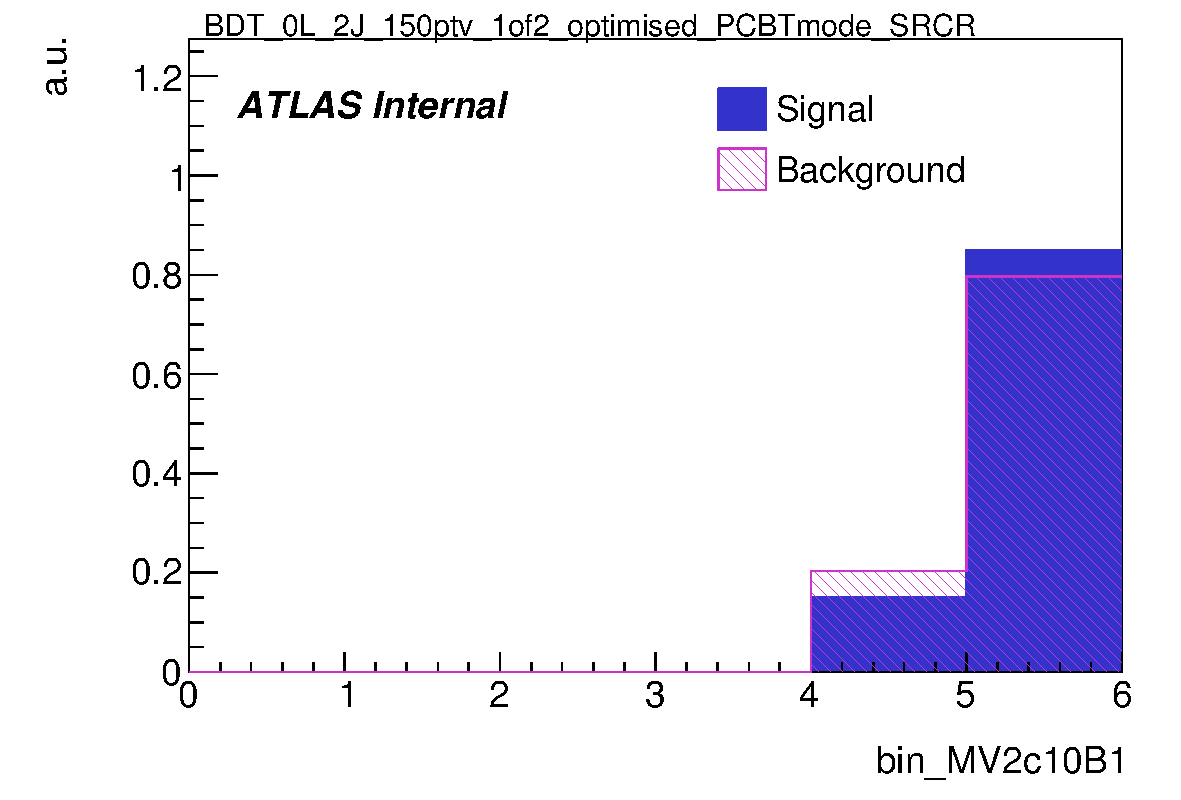
\includegraphics[width=0.33\linewidth]{0-lep-mva/Distr_SignalBackground_bin_MV2c10B1_BDT_0L_2J_150ptv_1of2_optimised_PCBTmode_SRCR-eps-converted-to}}
    \subfloat[]{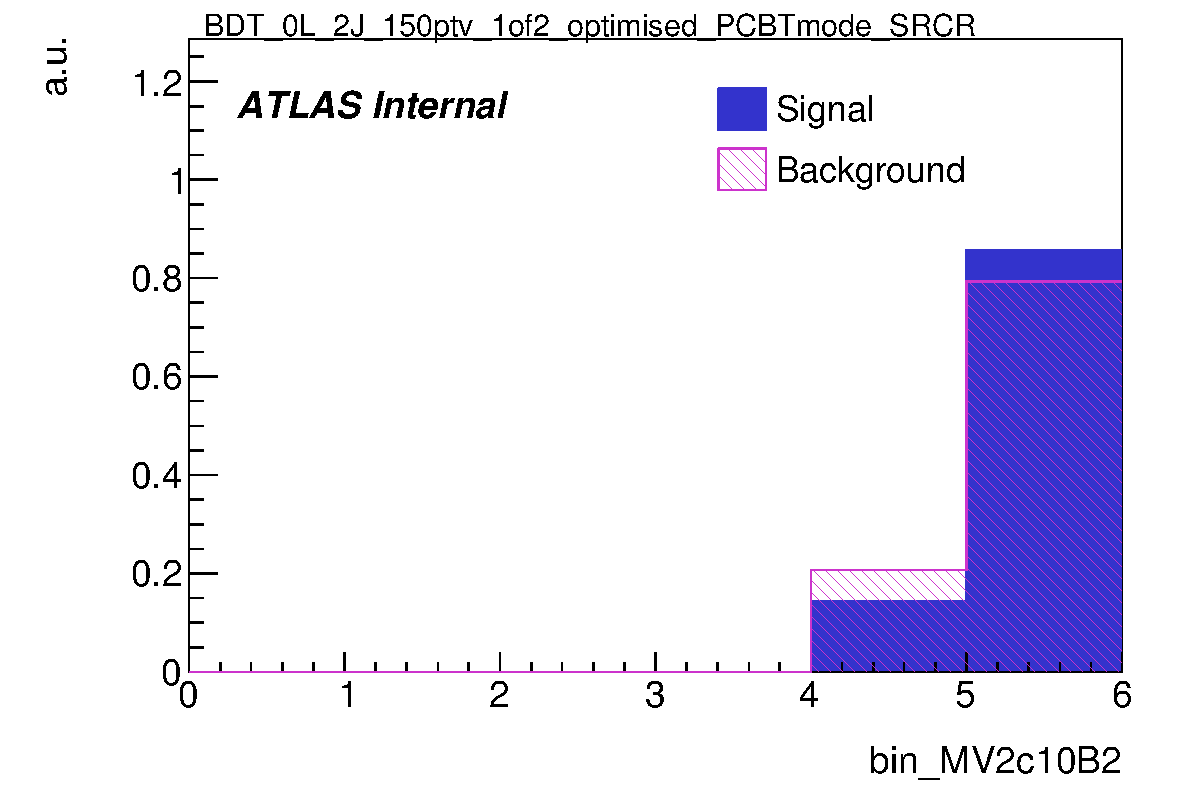
\includegraphics[width=0.33\linewidth]{0-lep-mva/Distr_SignalBackground_bin_MV2c10B2_BDT_0L_2J_150ptv_1of2_optimised_PCBTmode_SRCR-eps-converted-to}}
     \subfloat[]{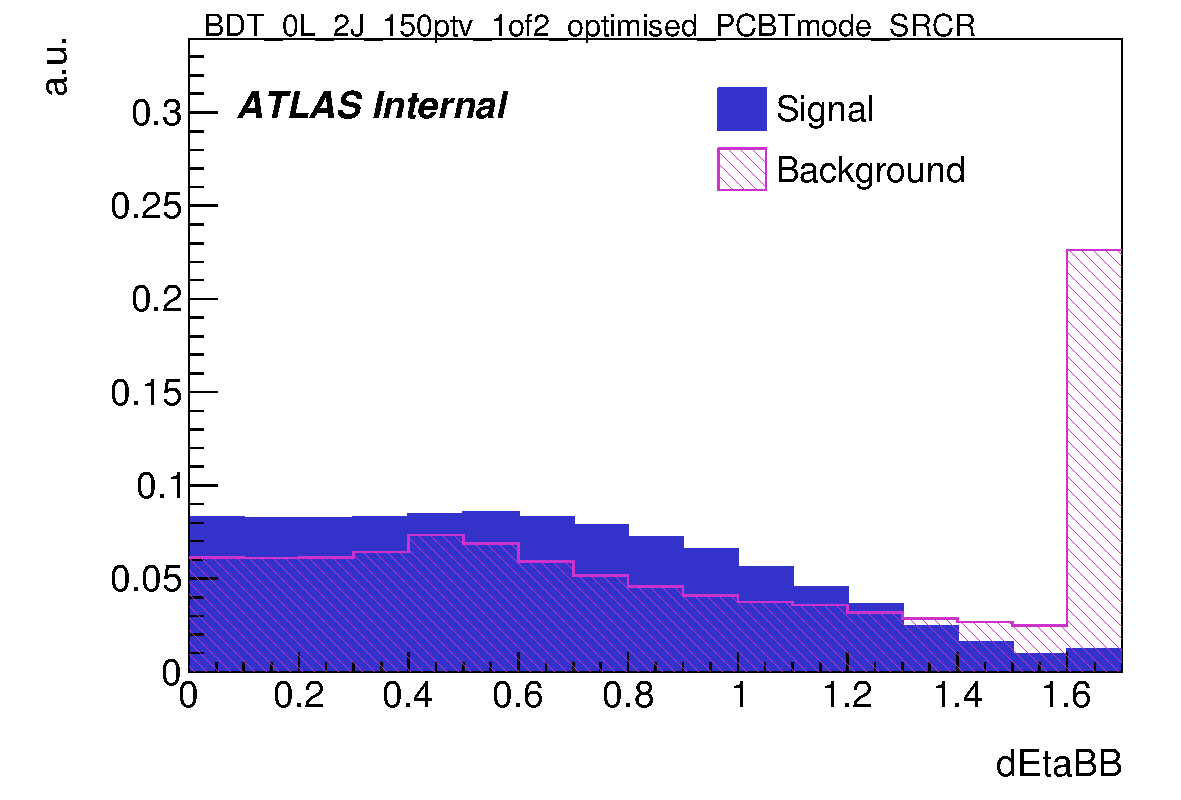
\includegraphics[width=0.33\linewidth]{0-lep-mva/Distr_SignalBackground_dEtaBB_BDT_0L_2J_150ptv_1of2_optimised_PCBTmode_SRCR-eps-converted-to}}\\
    \subfloat[]{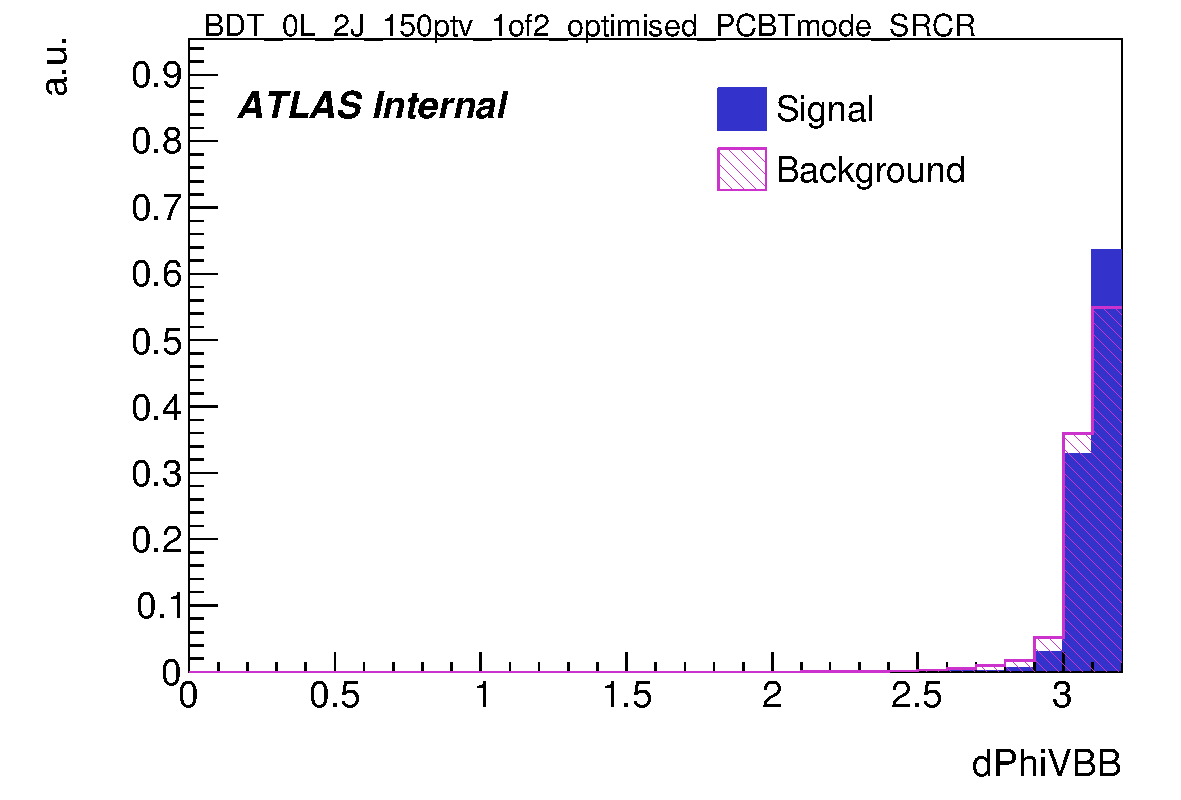
\includegraphics[width=0.33\linewidth]{0-lep-mva/Distr_SignalBackground_dPhiVBB_BDT_0L_2J_150ptv_1of2_optimised_PCBTmode_SRCR-eps-converted-to}}
    \subfloat[]{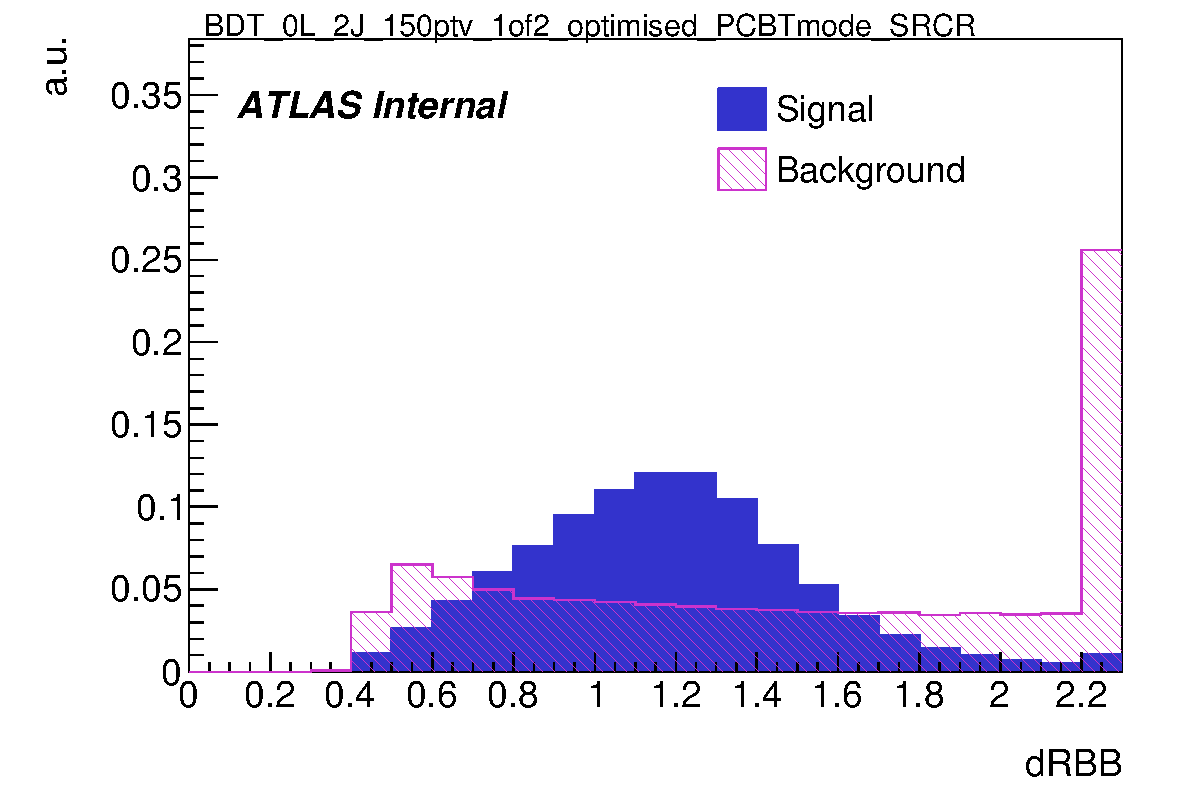
\includegraphics[width=0.33\linewidth]{0-lep-mva/Distr_SignalBackground_dRBB_BDT_0L_2J_150ptv_1of2_optimised_PCBTmode_SRCR-eps-converted-to}}
     \subfloat[]{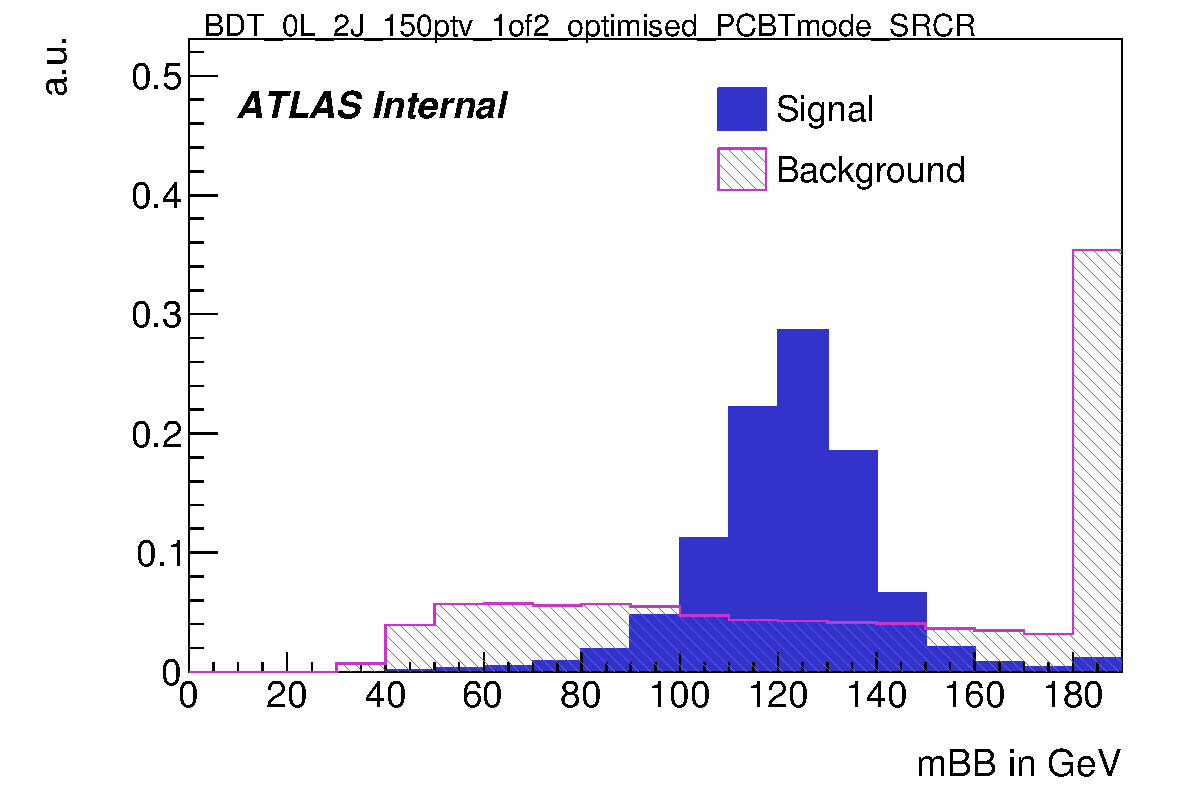
\includegraphics[width=0.33\linewidth]{0-lep-mva/Distr_SignalBackground_mBB_BDT_0L_2J_150ptv_1of2_optimised_PCBTmode_SRCR-eps-converted-to}}\\
    \subfloat[]{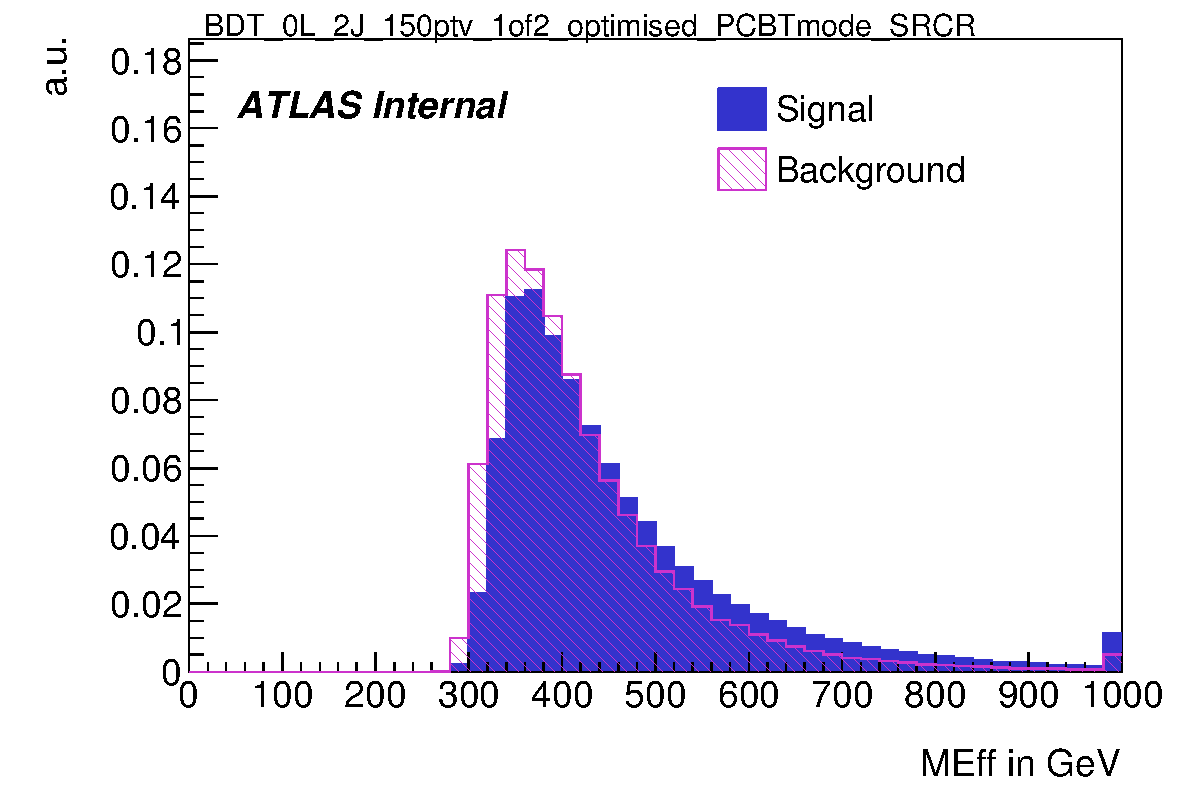
\includegraphics[width=0.33\linewidth]{0-lep-mva/Distr_SignalBackground_MEff_BDT_0L_2J_150ptv_1of2_optimised_PCBTmode_SRCR-eps-converted-to}}
     \subfloat[]{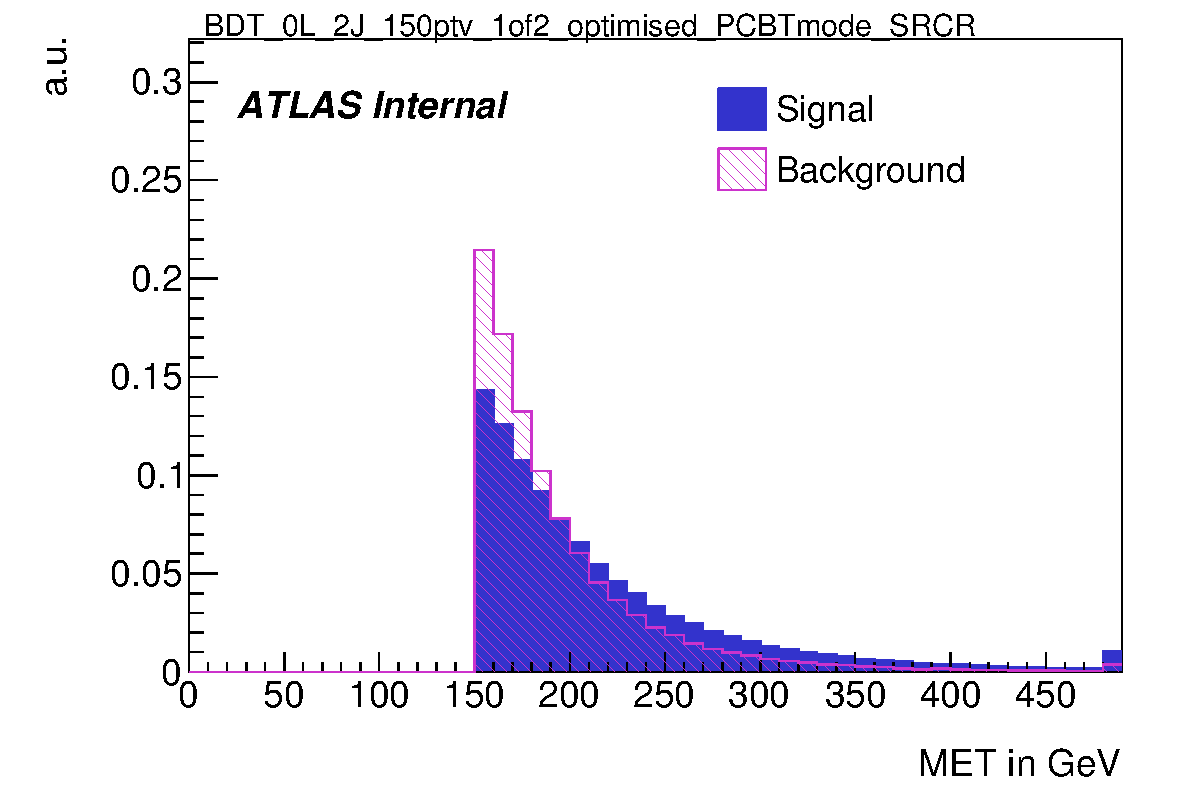
\includegraphics[width=0.33\linewidth]{0-lep-mva/Distr_SignalBackground_MET_BDT_0L_2J_150ptv_1of2_optimised_PCBTmode_SRCR-eps-converted-to}}          
    \subfloat[]{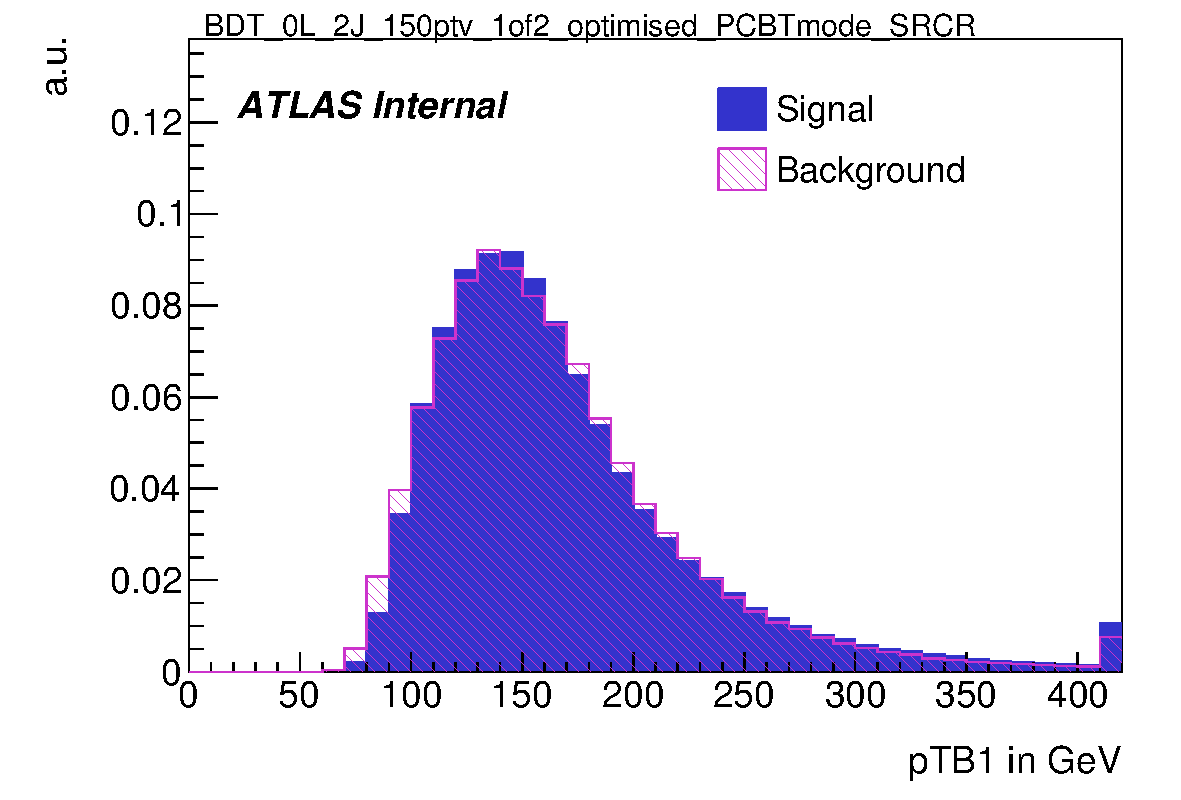
\includegraphics[width=0.33\linewidth]{0-lep-mva/Distr_SignalBackground_pTB1_BDT_0L_2J_150ptv_1of2_optimised_PCBTmode_SRCR-eps-converted-to}} \\
    \subfloat[]{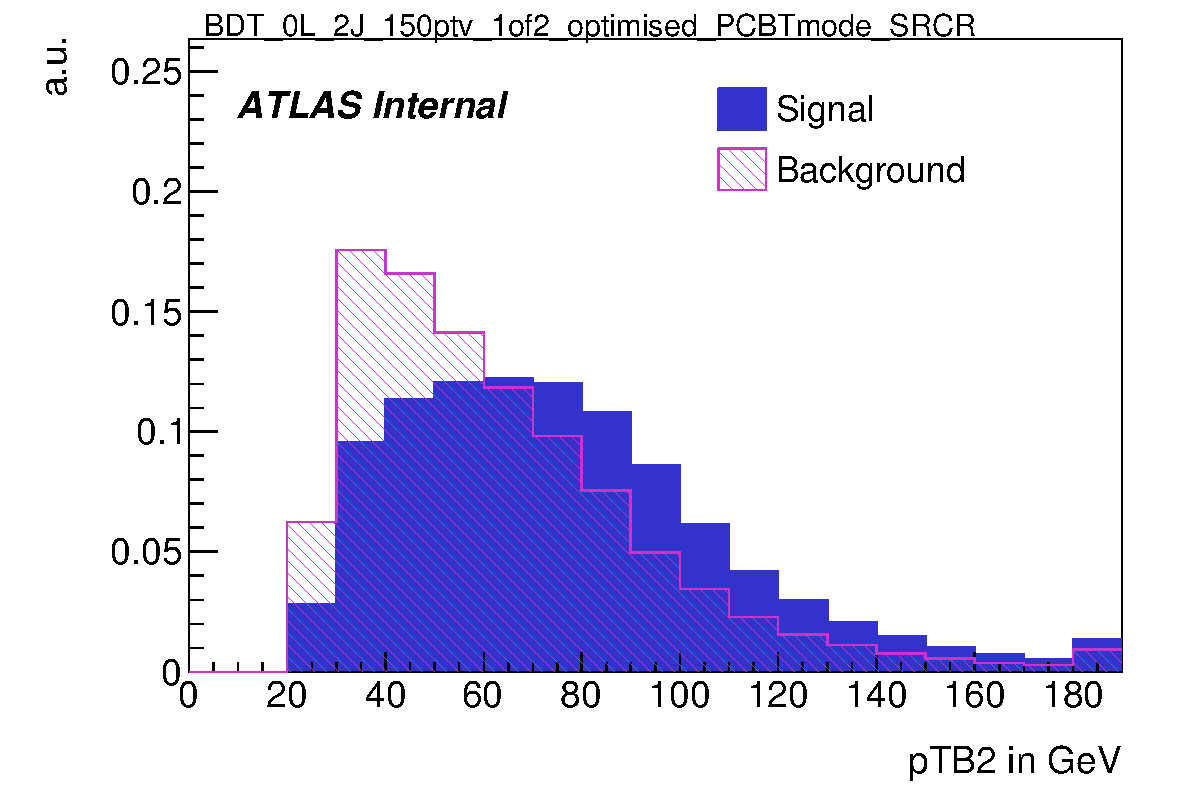
\includegraphics[width=0.33\linewidth]{0-lep-mva/Distr_SignalBackground_pTB2_BDT_0L_2J_150ptv_1of2_optimised_PCBTmode_SRCR-eps-converted-to}}   
    \subfloat[]{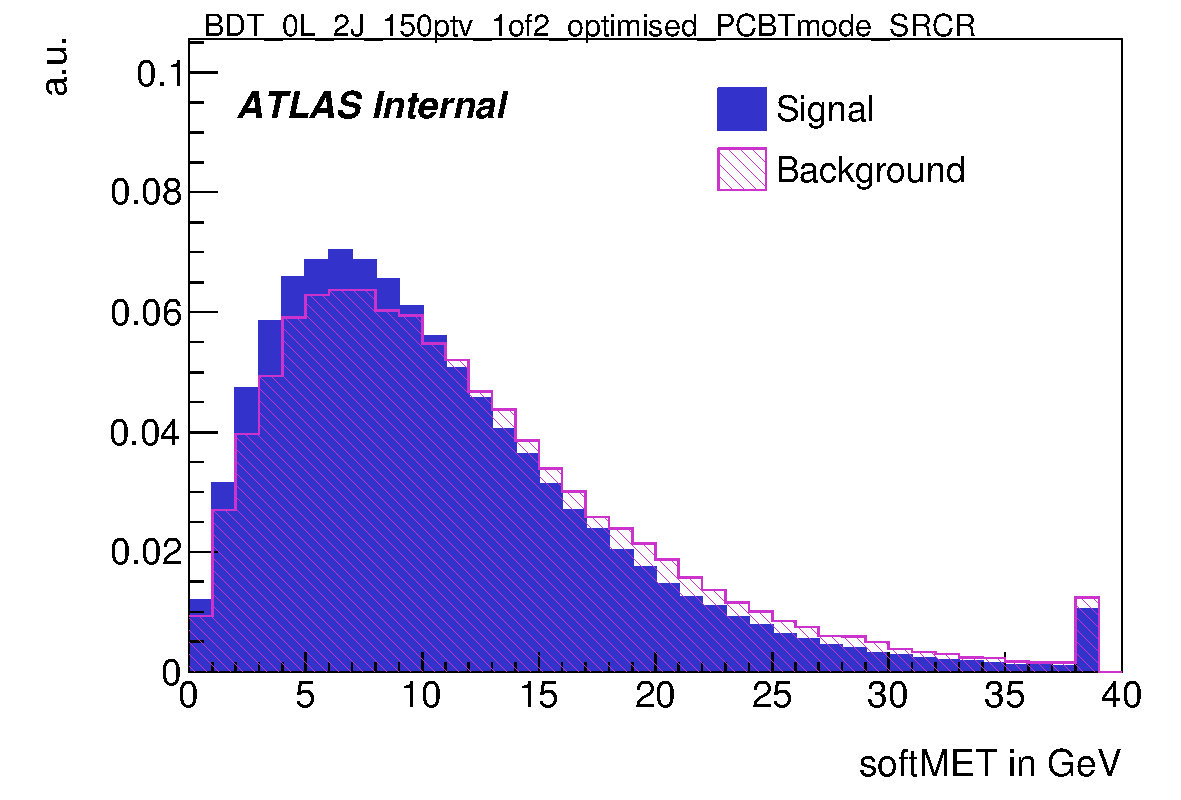
\includegraphics[width=0.33\linewidth]{0-lep-mva/Distr_SignalBackground_softMET_BDT_0L_2J_150ptv_1of2_optimised_PCBTmode_SRCR-eps-converted-to}}\\    
    \end{tabular}
    \caption[Inputs to the multi-variate analysis in the 0--lepton 2--jet
    region.]{Inputs to the multi-variate analysis in the 0--lepton 2--jet
      region. Signal events are shown in blue and background events are shown in
      red. The signal and background histograms have been normalised to the same
      area. The distributions only include events with $E_T^{\text{miss}}$ > 150
      \GeV.}
    \label{fig:bdtinputs-0lep}
\end{figure}

 \begin{figure}[htbp]
  \centering
  \begin{tabular}{cccc}
    \subfloat[]{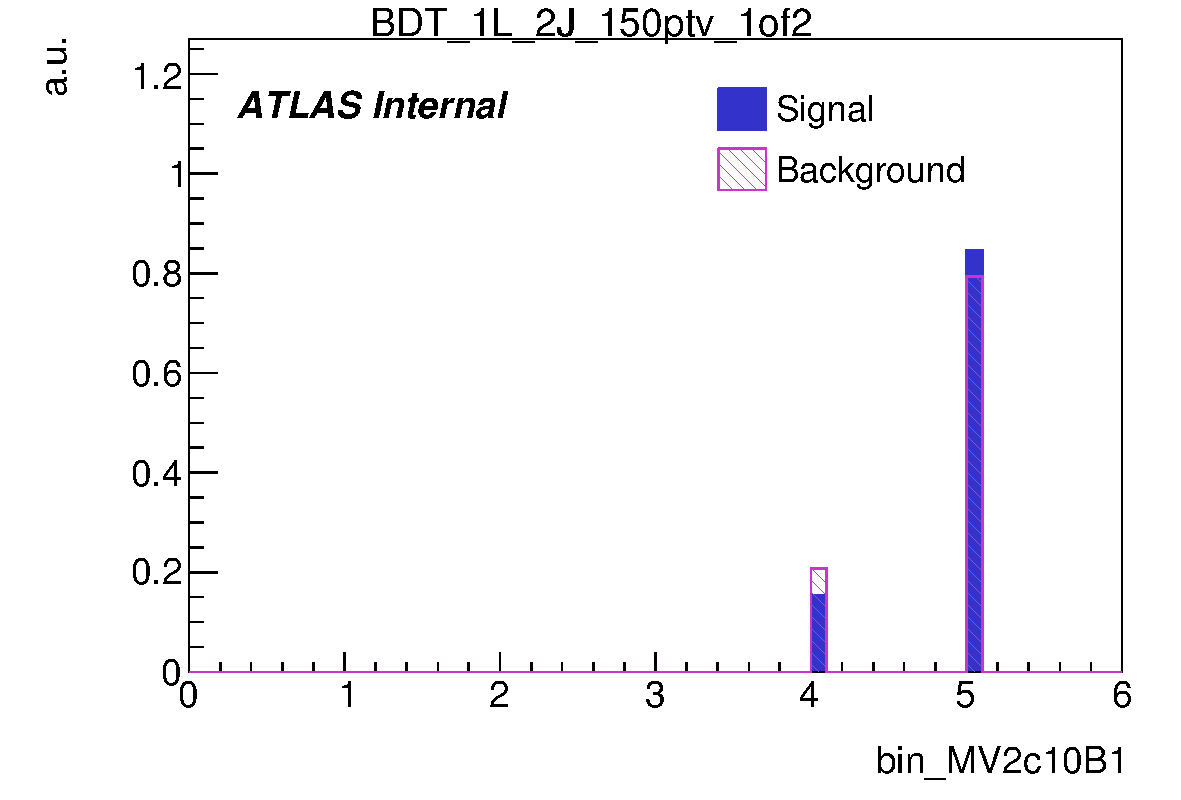
\includegraphics[width=0.3\linewidth]{1-lep-mva/Distr_SignalBackground_bin_MV2c10B1_BDT_1L_2J_150ptv_1of2-eps-converted-to}}
    \subfloat[]{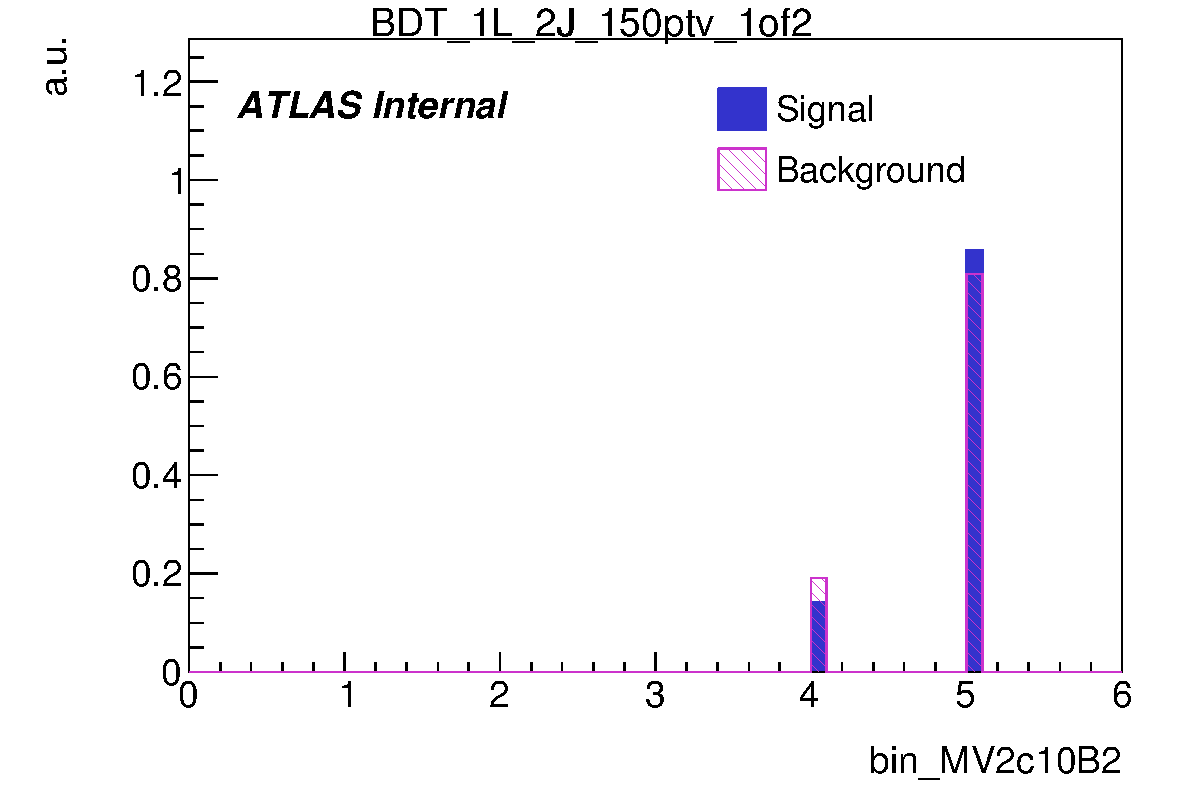
\includegraphics[width=0.3\linewidth]{1-lep-mva/Distr_SignalBackground_bin_MV2c10B2_BDT_1L_2J_150ptv_1of2-eps-converted-to}}
     \subfloat[]{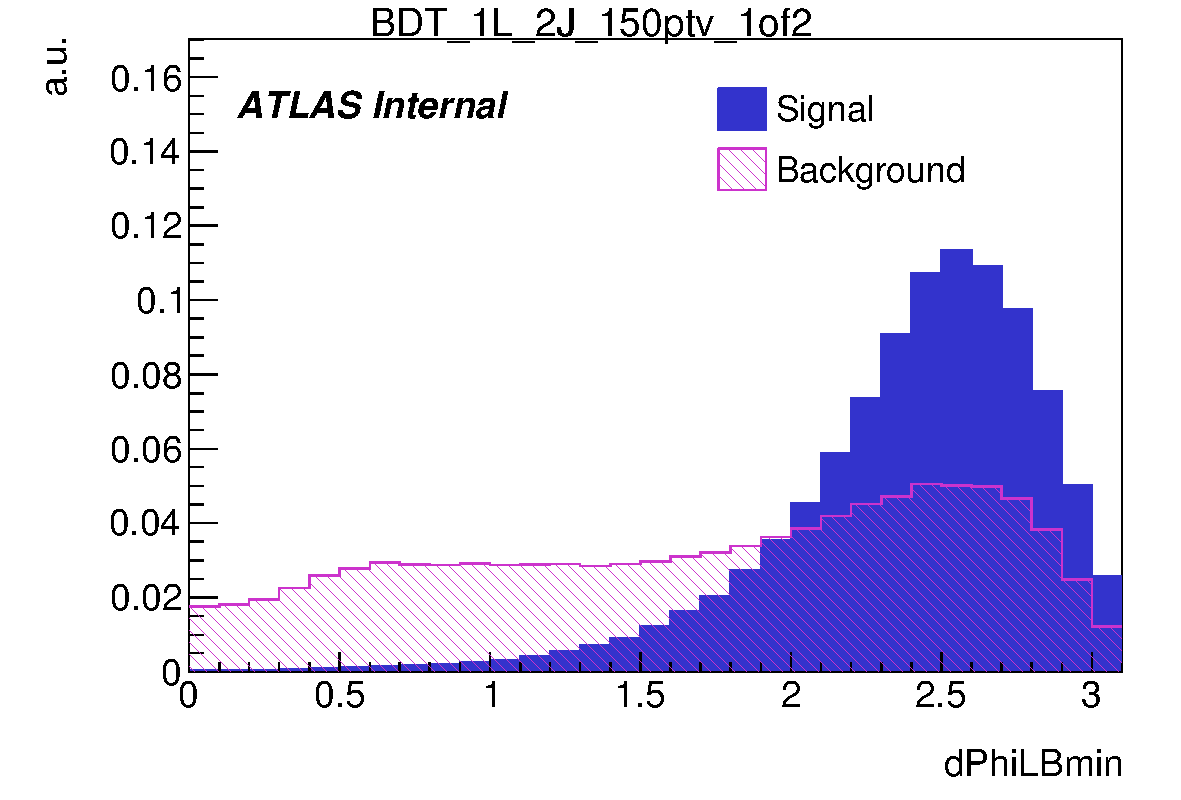
\includegraphics[width=0.3\linewidth]{1-lep-mva/Distr_SignalBackground_dPhiLBmin_BDT_1L_2J_150ptv_1of2-eps-converted-to}}\\
    \subfloat[]{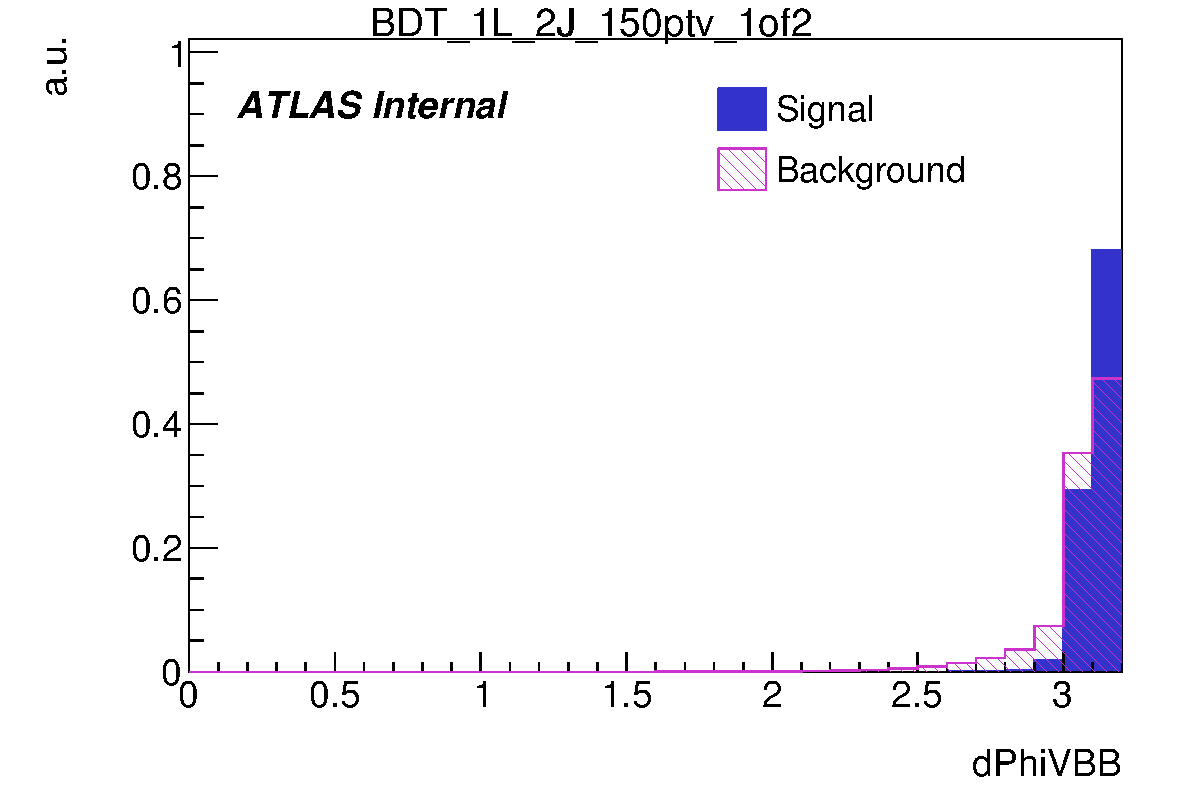
\includegraphics[width=0.3\linewidth]{1-lep-mva/Distr_SignalBackground_dPhiVBB_BDT_1L_2J_150ptv_1of2-eps-converted-to}}
    \subfloat[]{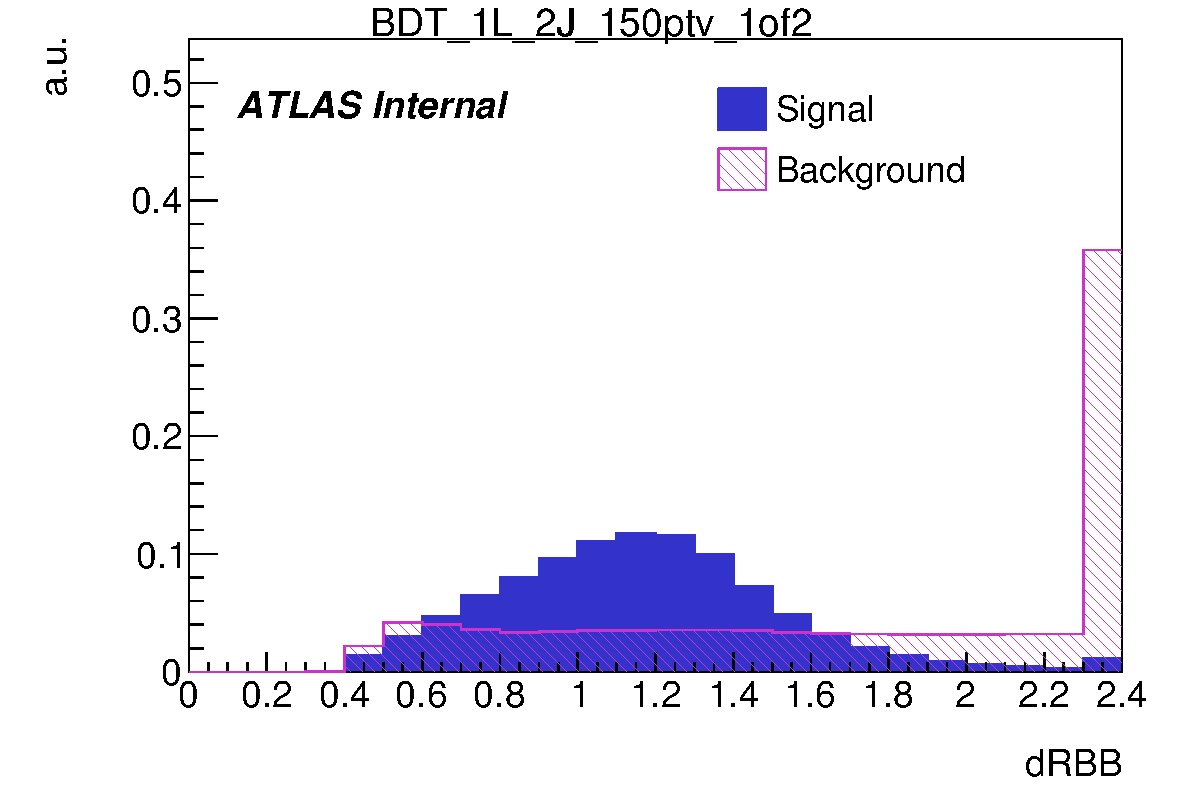
\includegraphics[width=0.3\linewidth]{1-lep-mva/Distr_SignalBackground_dRBB_BDT_1L_2J_150ptv_1of2-eps-converted-to}}
     \subfloat[]{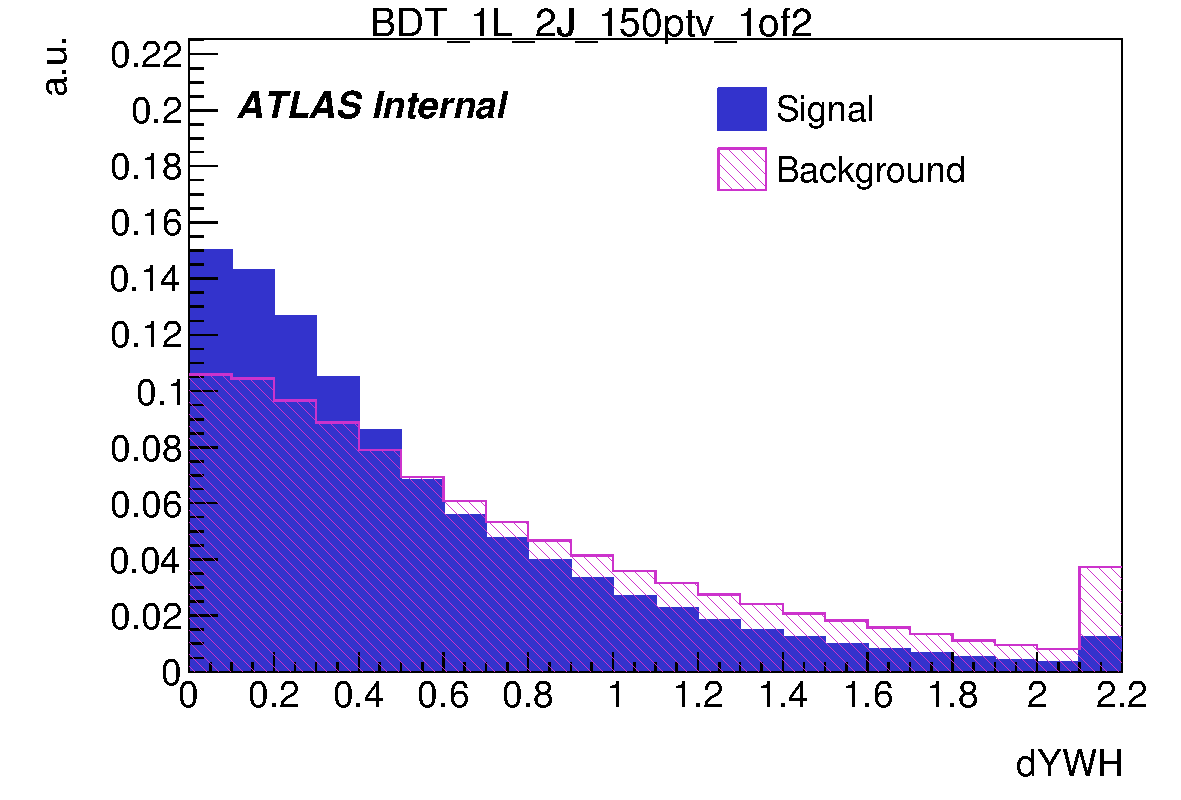
\includegraphics[width=0.3\linewidth]{1-lep-mva/Distr_SignalBackground_dYWH_BDT_1L_2J_150ptv_1of2-eps-converted-to}}\\
    \subfloat[]{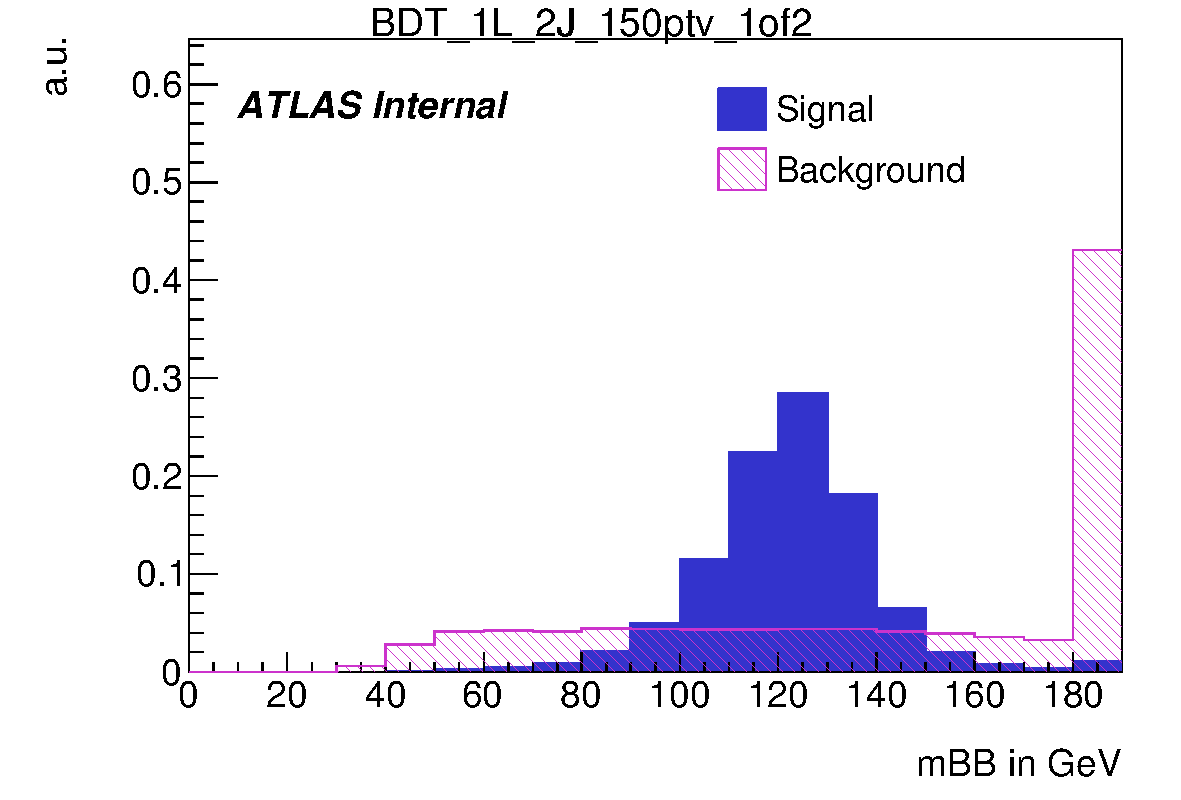
\includegraphics[width=0.3\linewidth]{1-lep-mva/Distr_SignalBackground_mBB_BDT_1L_2J_150ptv_1of2-eps-converted-to}}
     \subfloat[]{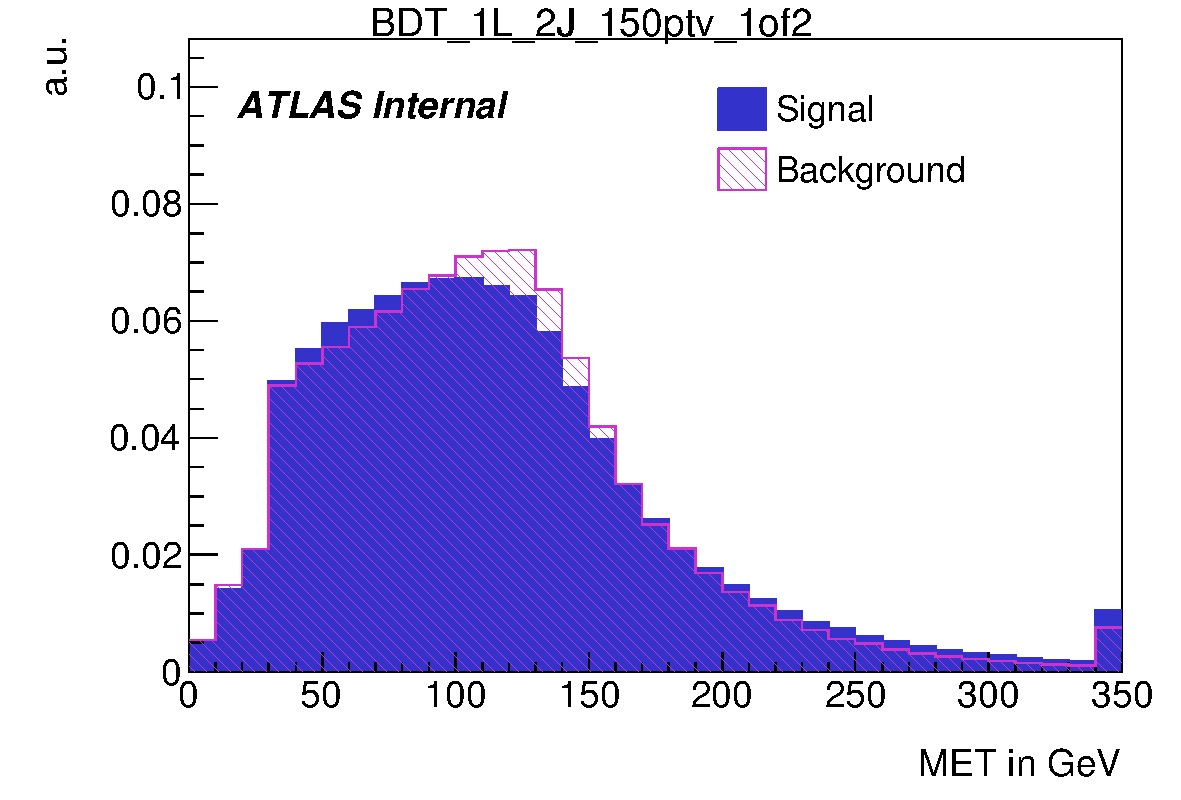
\includegraphics[width=0.3\linewidth]{1-lep-mva/Distr_SignalBackground_MET_BDT_1L_2J_150ptv_1of2-eps-converted-to}}          
    \subfloat[]{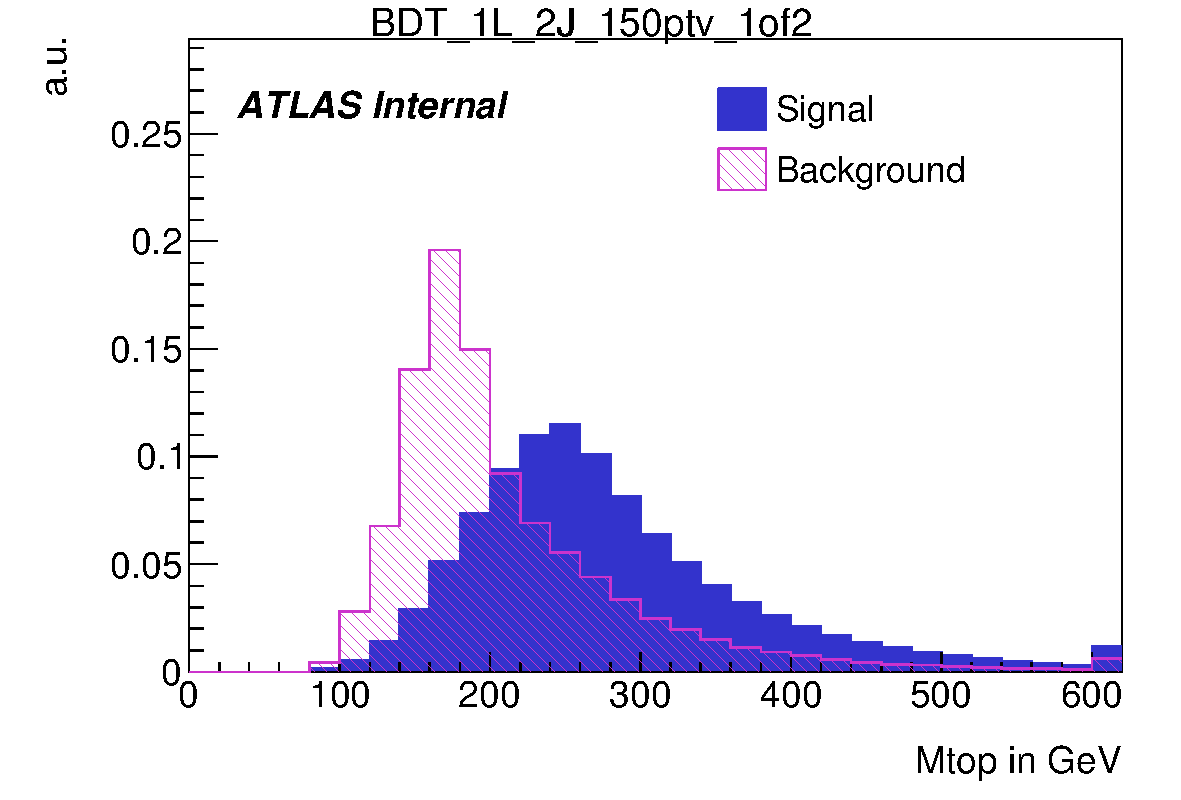
\includegraphics[width=0.3\linewidth]{1-lep-mva/Distr_SignalBackground_Mtop_BDT_1L_2J_150ptv_1of2-eps-converted-to}} \\
    \subfloat[]{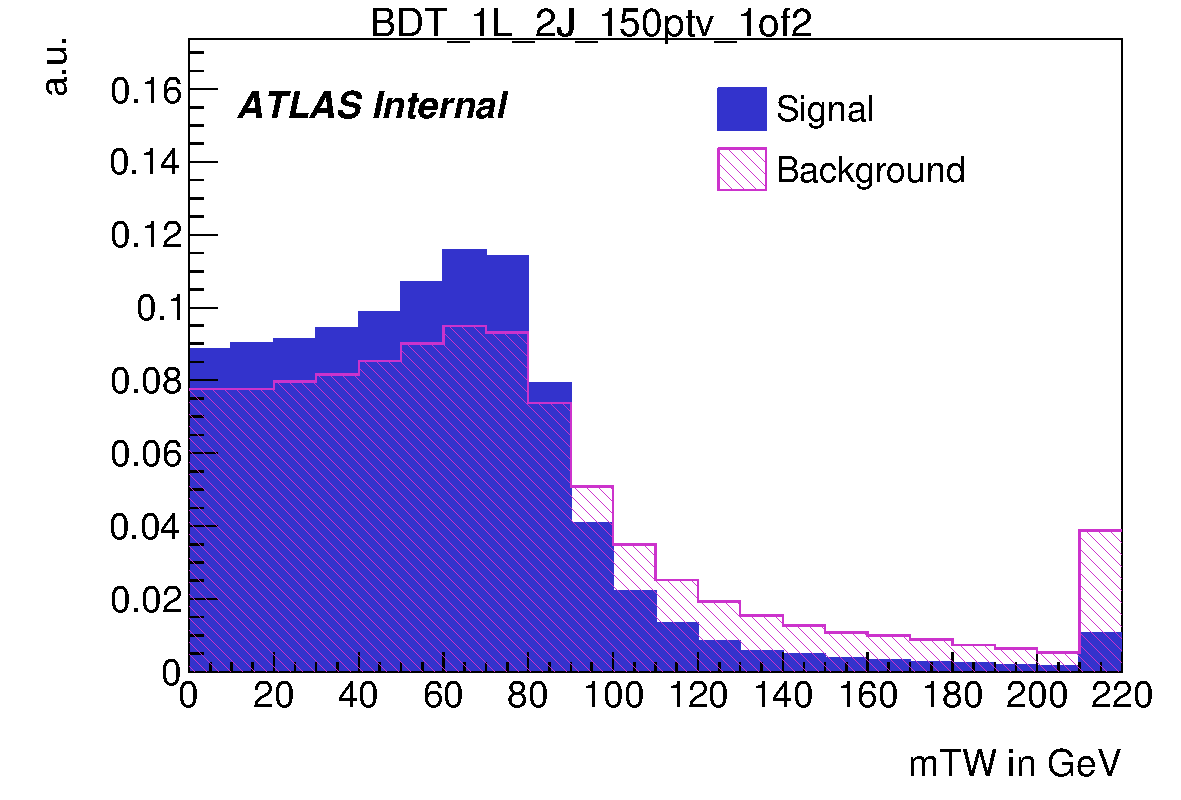
\includegraphics[width=0.3\linewidth]{1-lep-mva/Distr_SignalBackground_mTW_BDT_1L_2J_150ptv_1of2-eps-converted-to}}   
    \subfloat[]{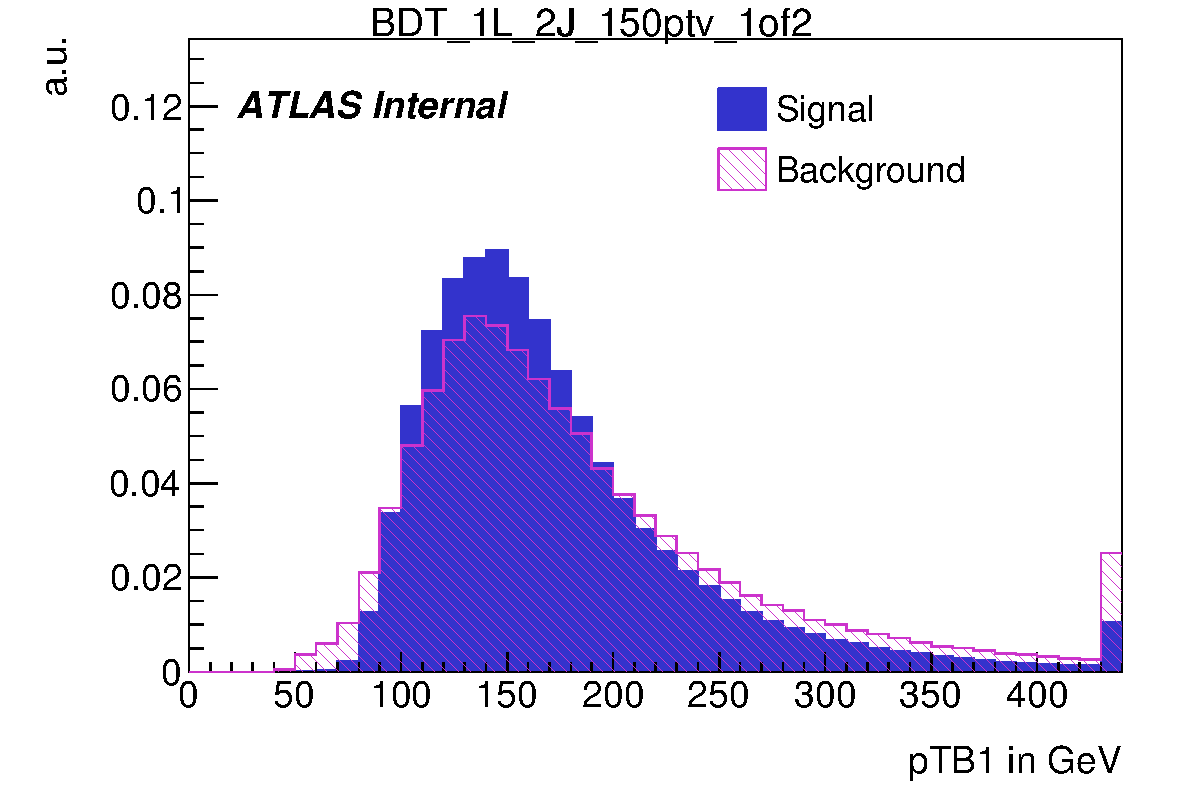
\includegraphics[width=0.3\linewidth]{1-lep-mva/Distr_SignalBackground_pTB1_BDT_1L_2J_150ptv_1of2-eps-converted-to}}
    \subfloat[]{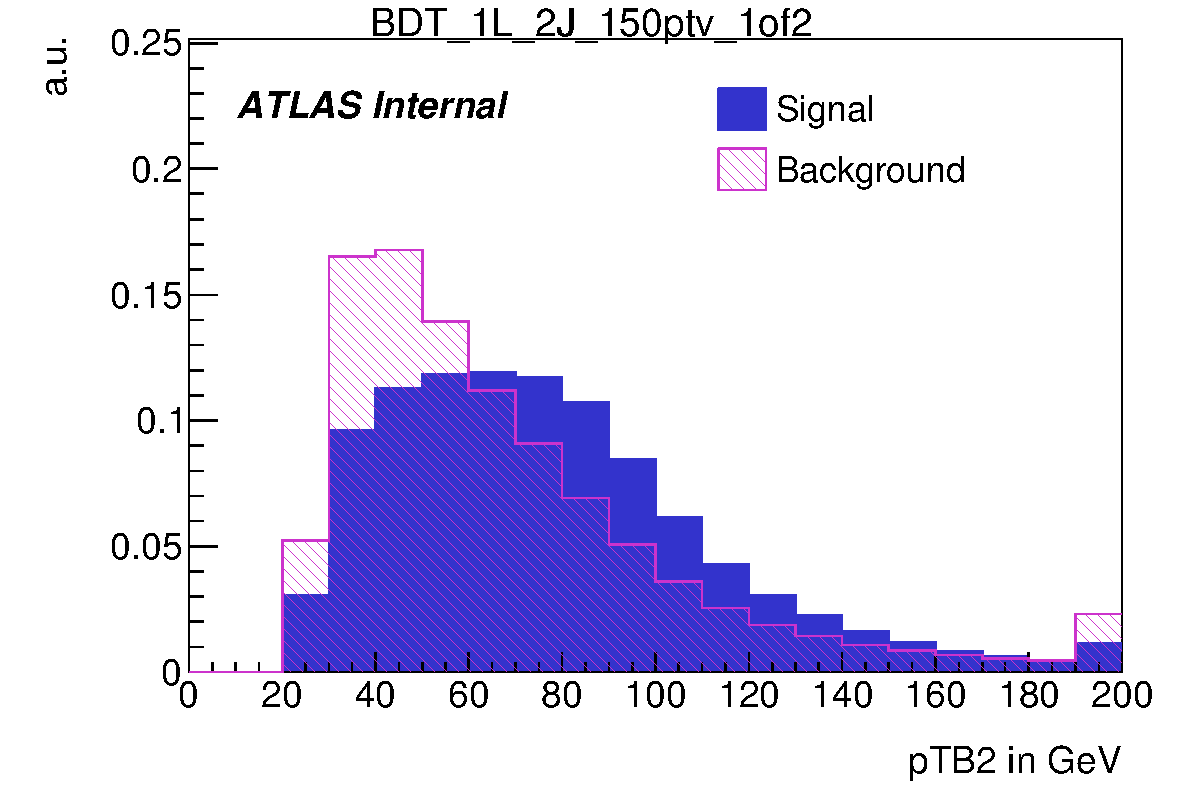
\includegraphics[width=0.3\linewidth]{1-lep-mva/Distr_SignalBackground_pTB2_BDT_1L_2J_150ptv_1of2-eps-converted-to}}\\   
    \subfloat[]{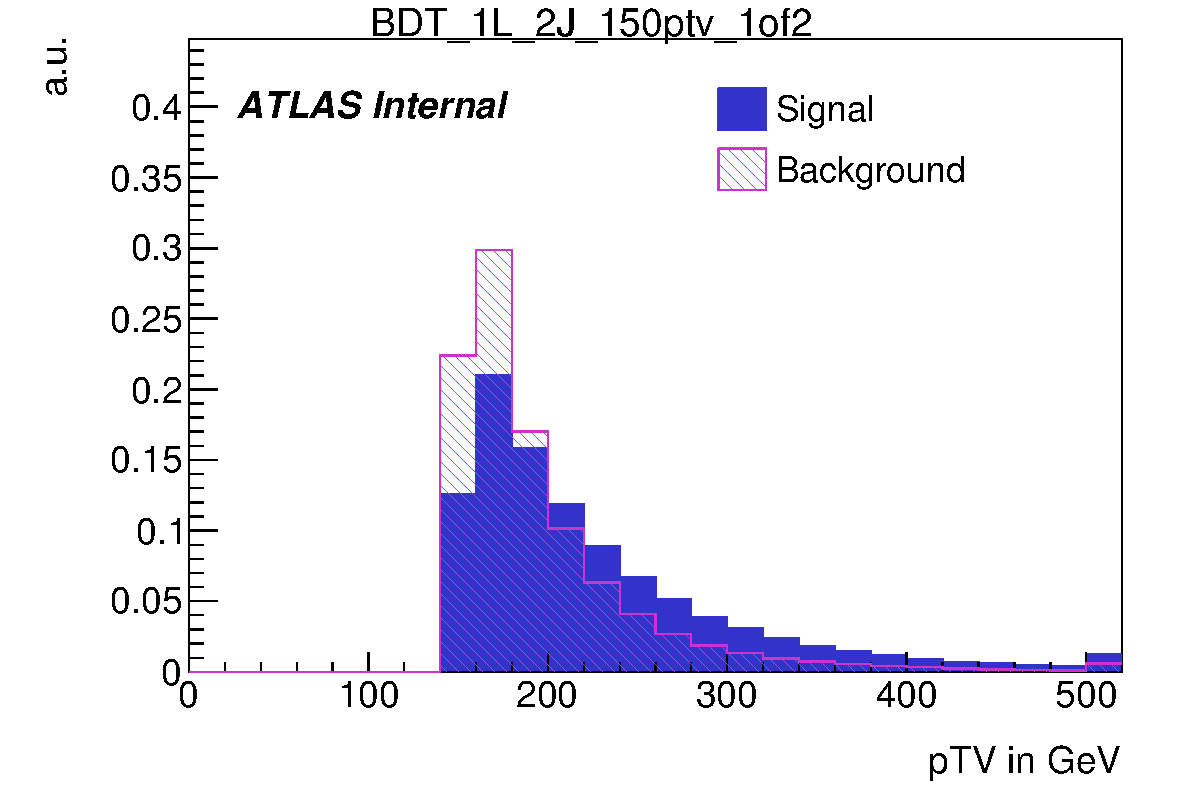
\includegraphics[width=0.3\linewidth]{1-lep-mva/Distr_SignalBackground_pTV_BDT_1L_2J_150ptv_1of2-eps-converted-to}} 
    \end{tabular}
    \caption[Inputs to the multi-variate analysis in the 1--lepton 2--jet
    region.]{Inputs to the multi-variate analysis in the 1--lepton 2--jet
      region. Signal events are shown in blue and background events are shown in
      red. The signal and background histograms have been normalised to the same
      area.The distributions only include events with $p_T^{W}$ > 150
      \GeV.}
    \label{fig:bdtinputs-1lep}
\end{figure}

 \begin{figure}[htbp]
  \centering
  \begin{tabular}{cccc}
    \subfloat[]{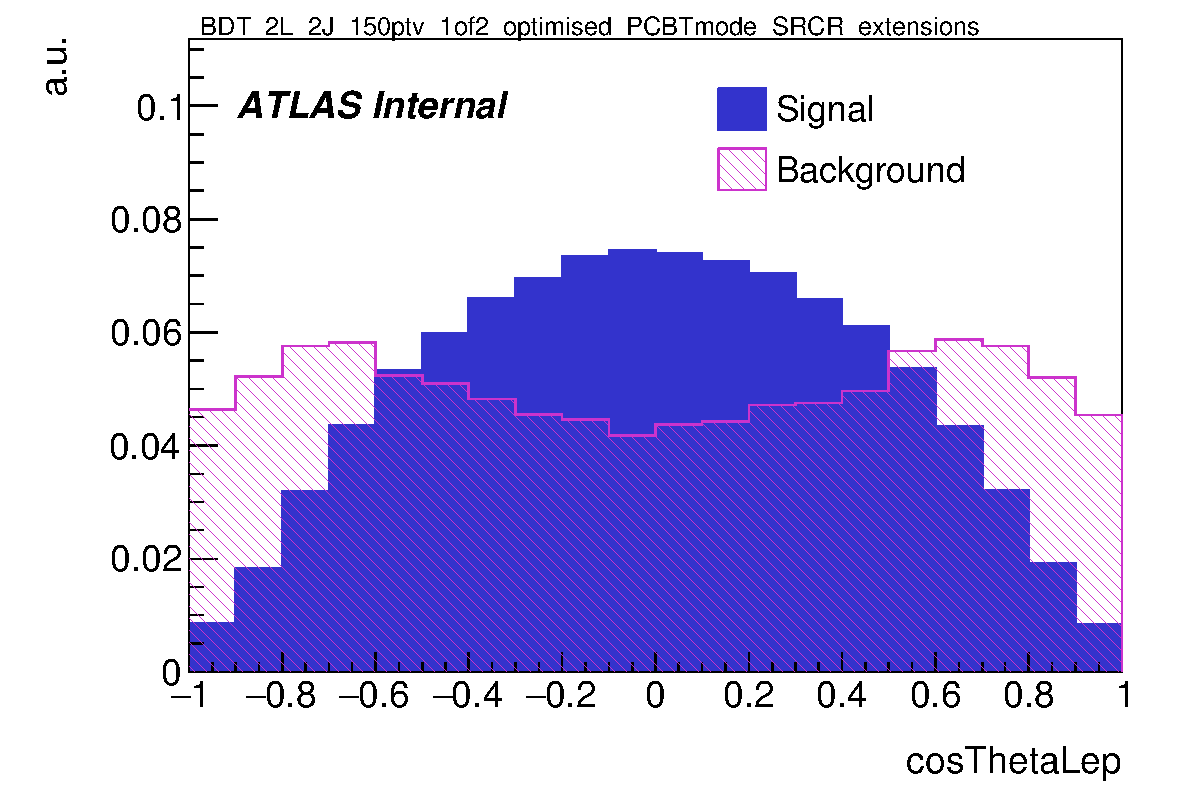
\includegraphics[width=0.33\linewidth]{2-lep-mva/Distr_SignalBackground_cosThetaLep_BDT_2L_2J_150ptv_1of2_optimised_PCBTmode_SRCR_extensions-eps-converted-to}}
    \subfloat[]{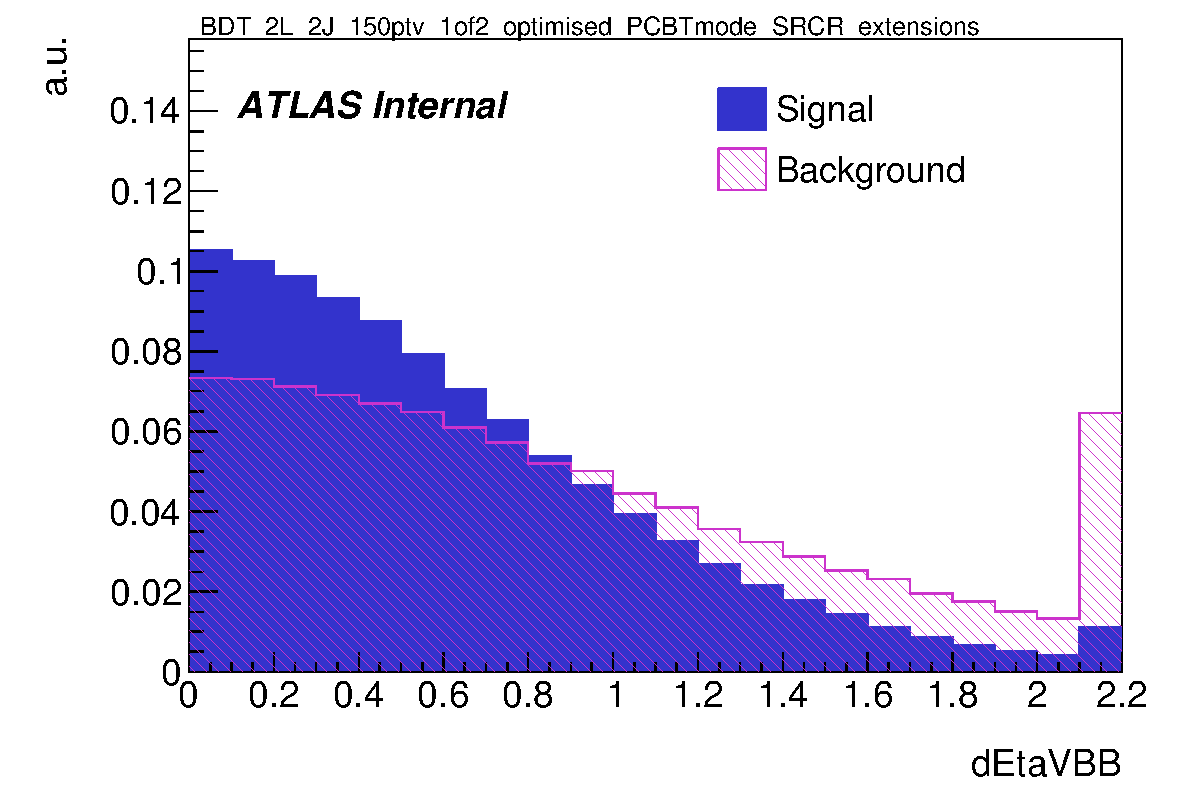
\includegraphics[width=0.33\linewidth]{2-lep-mva/Distr_SignalBackground_dEtaVBB_BDT_2L_2J_150ptv_1of2_optimised_PCBTmode_SRCR_extensions-eps-converted-to}}
     \subfloat[]{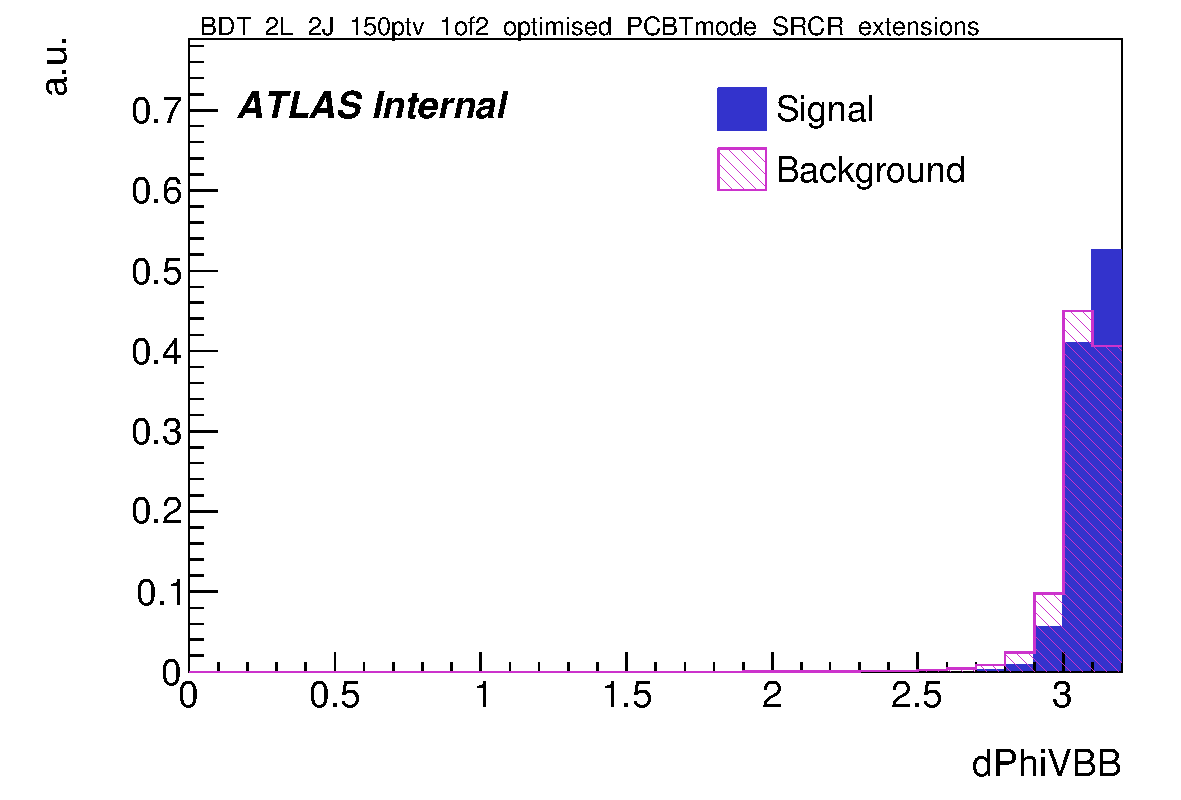
\includegraphics[width=0.33\linewidth]{2-lep-mva/Distr_SignalBackground_dPhiVBB_BDT_2L_2J_150ptv_1of2_optimised_PCBTmode_SRCR_extensions-eps-converted-to}}\\
    \subfloat[]{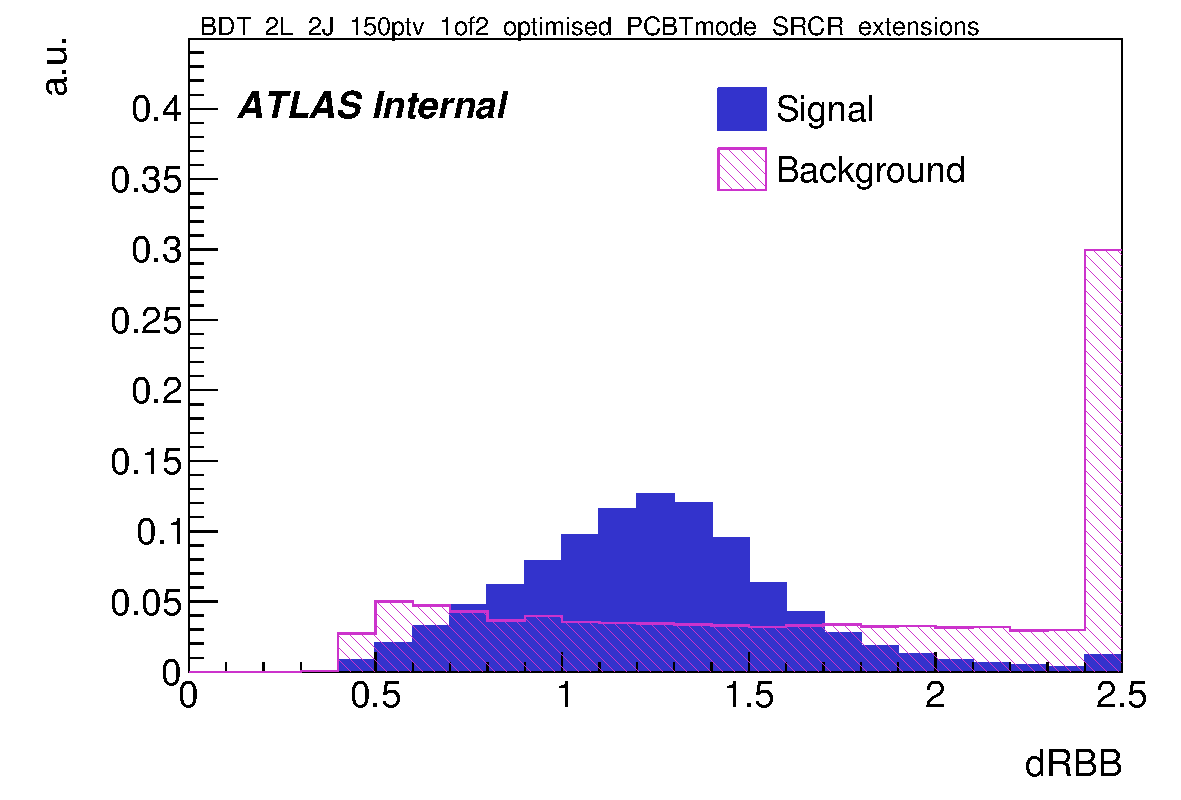
\includegraphics[width=0.33\linewidth]{2-lep-mva/Distr_SignalBackground_dRBB_BDT_2L_2J_150ptv_1of2_optimised_PCBTmode_SRCR_extensions-eps-converted-to}}
    \subfloat[]{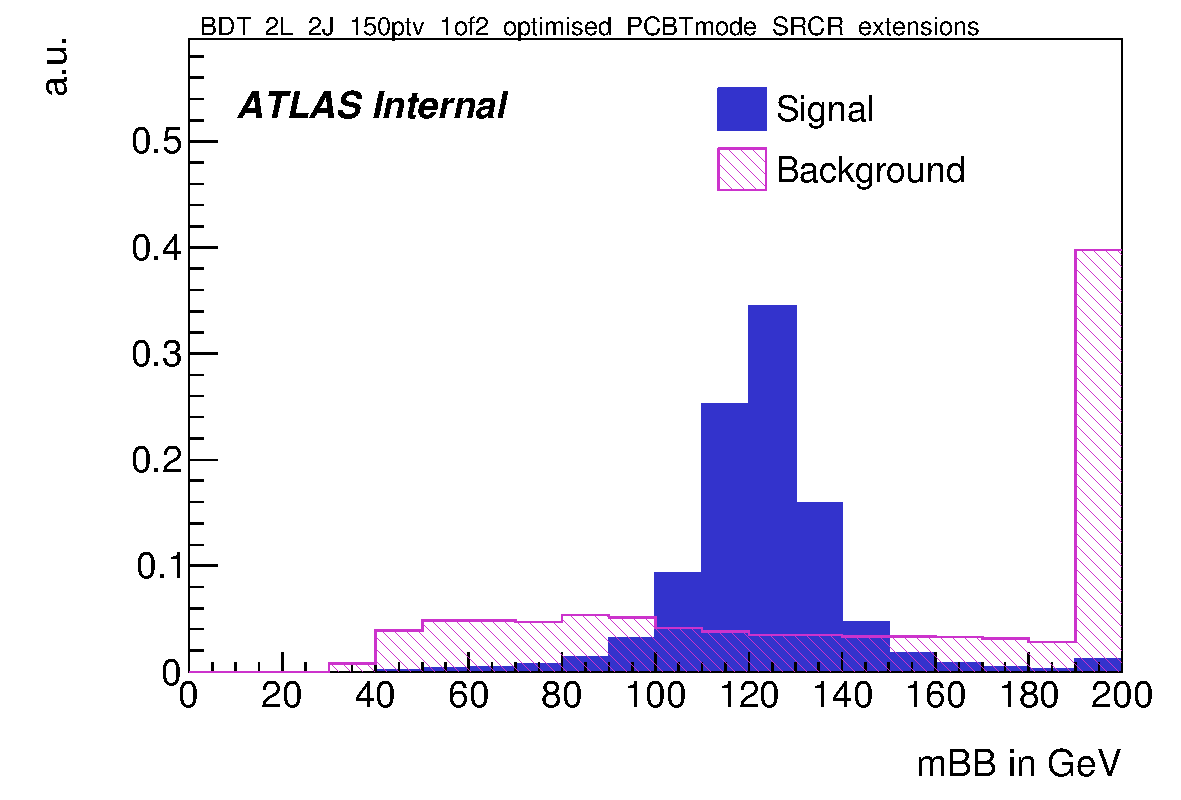
\includegraphics[width=0.33\linewidth]{2-lep-mva/Distr_SignalBackground_mBB_BDT_2L_2J_150ptv_1of2_optimised_PCBTmode_SRCR_extensions-eps-converted-to}}
     \subfloat[]{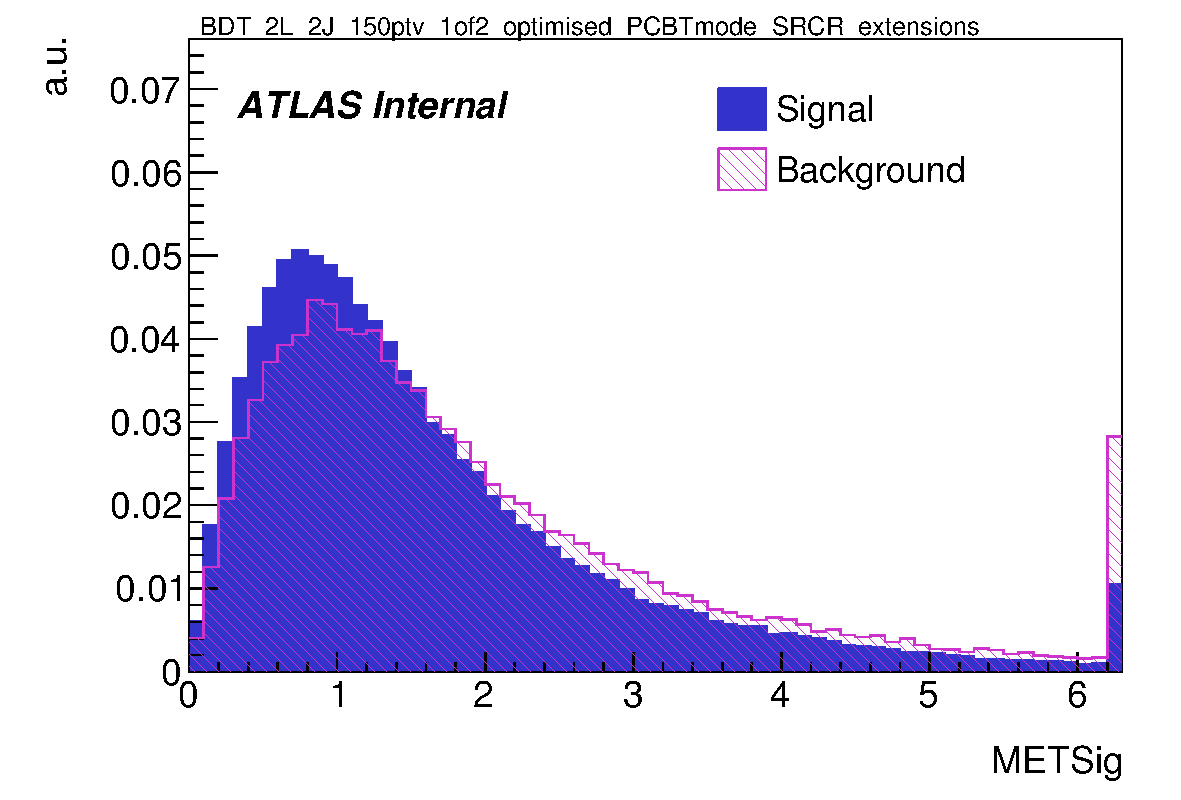
\includegraphics[width=0.33\linewidth]{2-lep-mva/Distr_SignalBackground_METSig_BDT_2L_2J_150ptv_1of2_optimised_PCBTmode_SRCR_extensions-eps-converted-to}}\\
    \subfloat[]{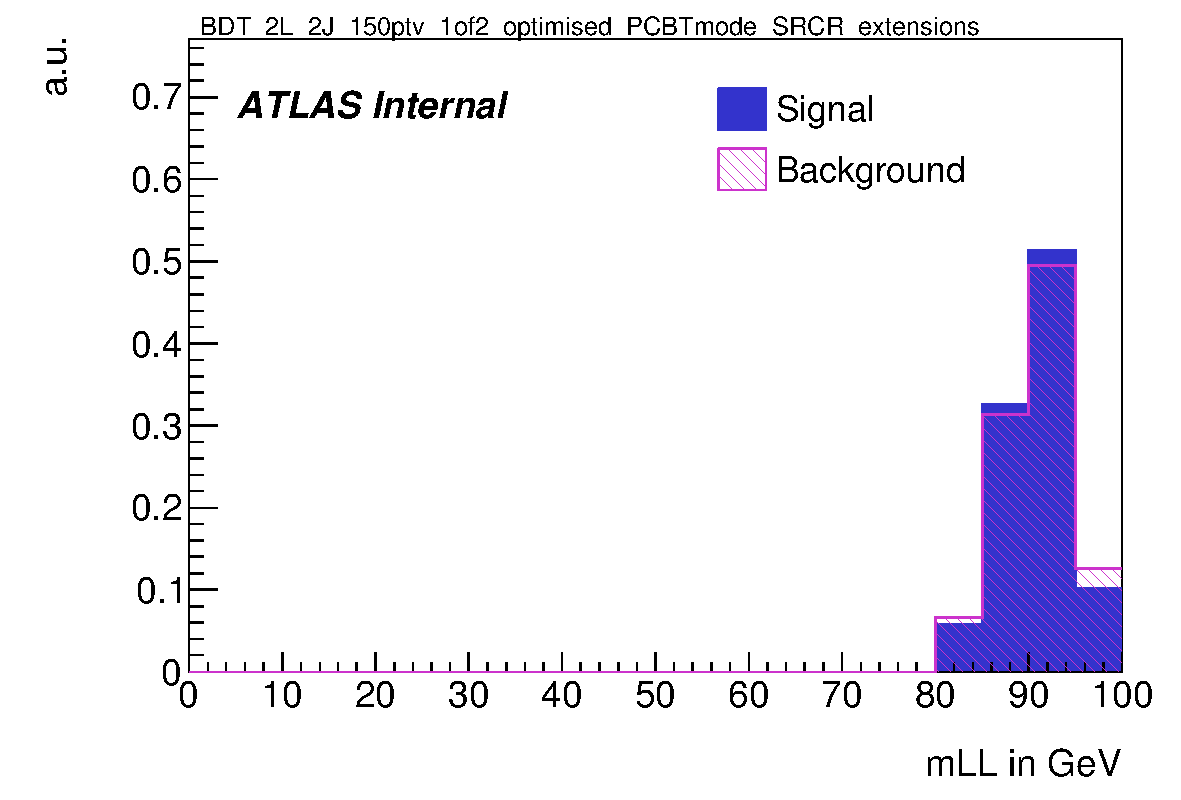
\includegraphics[width=0.33\linewidth]{2-lep-mva/Distr_SignalBackground_mLL_BDT_2L_2J_150ptv_1of2_optimised_PCBTmode_SRCR_extensions-eps-converted-to}}
     \subfloat[]{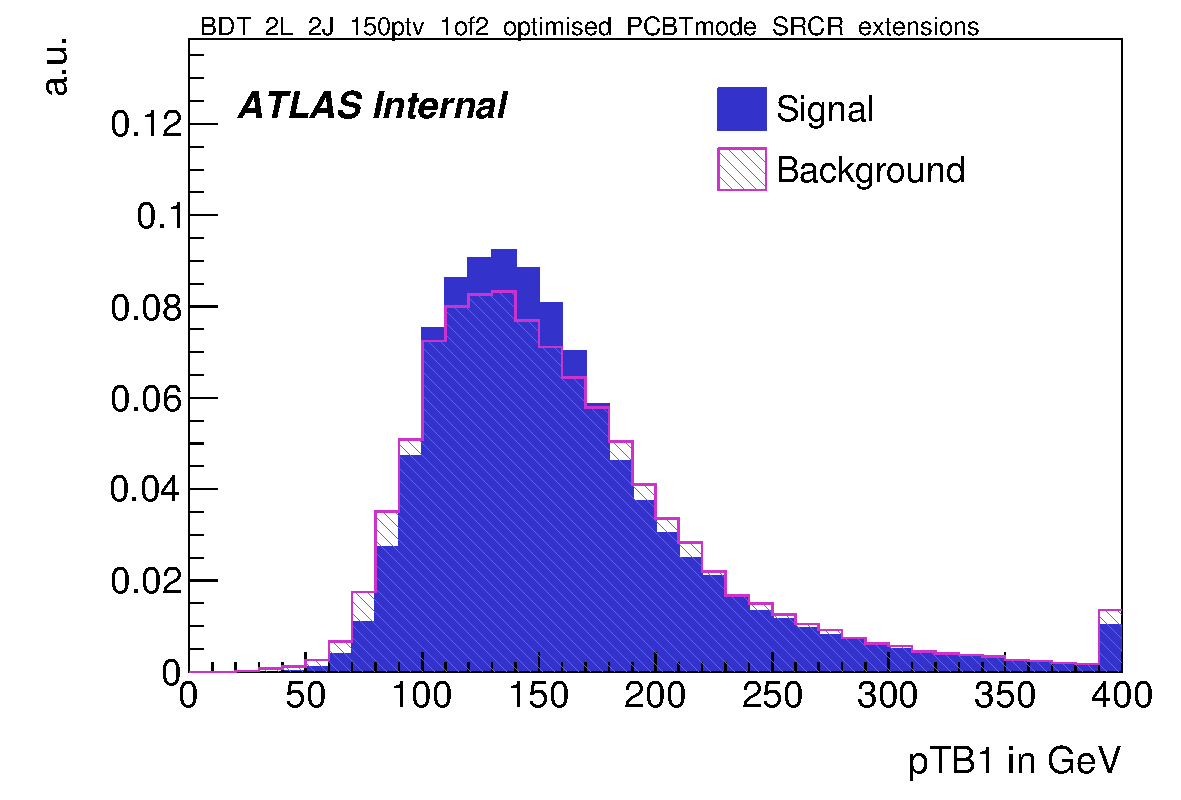
\includegraphics[width=0.33\linewidth]{2-lep-mva/Distr_SignalBackground_pTB1_BDT_2L_2J_150ptv_1of2_optimised_PCBTmode_SRCR_extensions-eps-converted-to}}          
    \subfloat[]{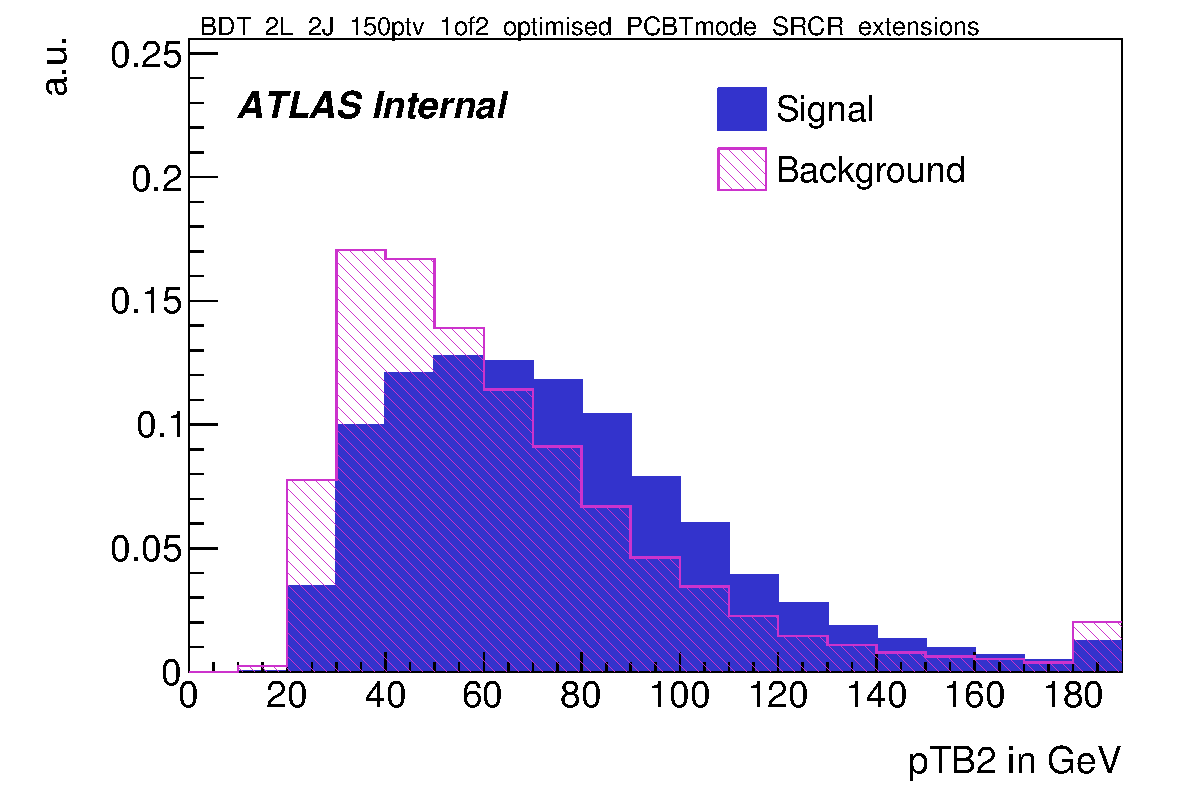
\includegraphics[width=0.33\linewidth]{2-lep-mva/Distr_SignalBackground_pTB2_BDT_2L_2J_150ptv_1of2_optimised_PCBTmode_SRCR_extensions-eps-converted-to}} \\
    \subfloat[]{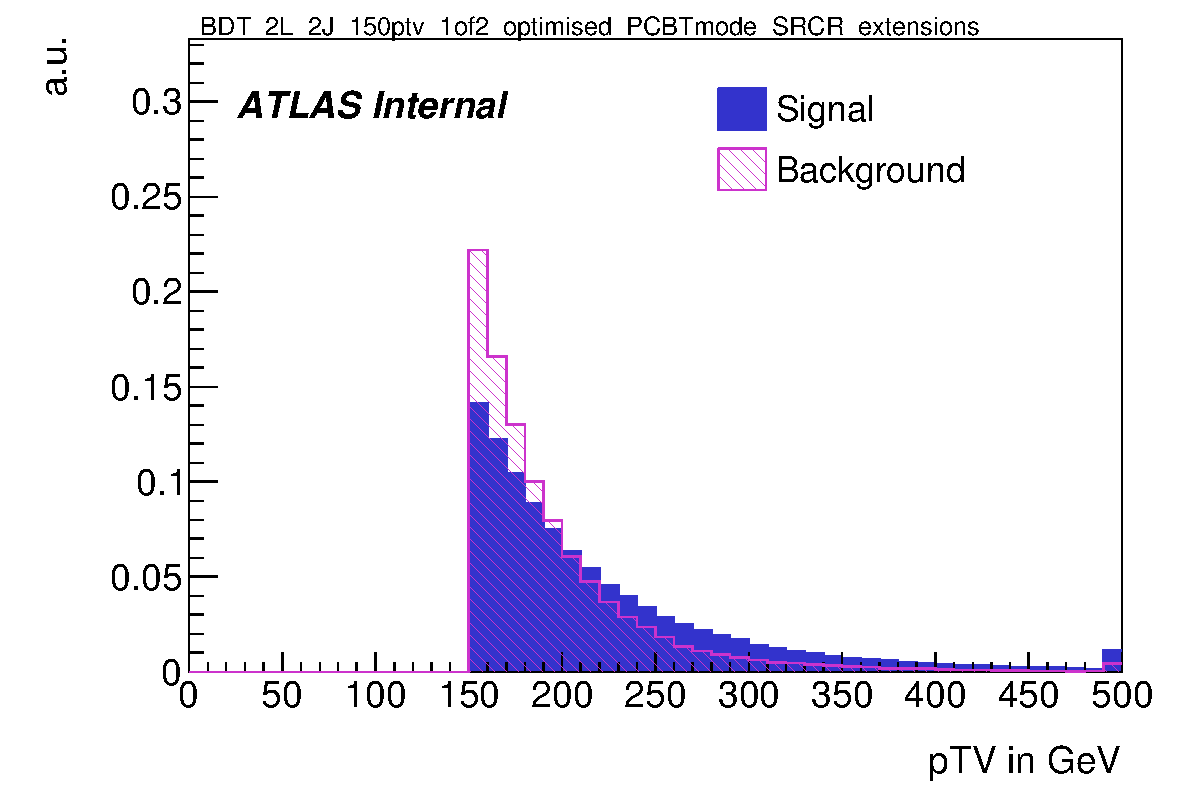
\includegraphics[width=0.33\linewidth]{2-lep-mva/Distr_SignalBackground_pTV_BDT_2L_2J_150ptv_1of2_optimised_PCBTmode_SRCR_extensions-eps-converted-to}}   
    \end{tabular}
    \caption[Inputs to the multi-variate analysis in the 2--lepton 2--jet
    region.]{Inputs to the multi-variate analysis in the 2--lepton 2--jet
      region. Signal events are shown in blue and background events are shown in
      red. The signal and background histograms have been normalised to the same
      area.The distributions only include events with $p_T^{Z}$ > 150
      \GeV.}
    \label{fig:bdtinputs-2lep}
\end{figure}


- What is the performance like?

- Transformation

\section{Pre-fit plots}
\label{sec:prefit}

This section shows the pre-fit distributions of the Monte-Carlo prediction
versus the data in every analysis region that enters into the profile-likelihood
fit. Figures~\ref{fig:0lep-2jet-prefit},~\ref{fig:0lep-3jet-prefit} show the
distributions in the 0--lepton channel in the 2--jet and 3--jet regions
respectively. Figures~\ref{fig:1lep-2jet-prefit},~\ref{fig:1lep-3jet-prefit} show the
distributions in the 1--lepton channel in the 2--jet and 3--jet regions
respectively. Figures~\ref{fig:2lep-2jet-prefit},~\ref{fig:2lep-3pjet-prefit} show the
distributions in the 2--lepton channel in the 2--jet and 3+--jet regions
respectively.
\begin{figure}
  \centering
  \begin{tabular}{cc}
    % top row
    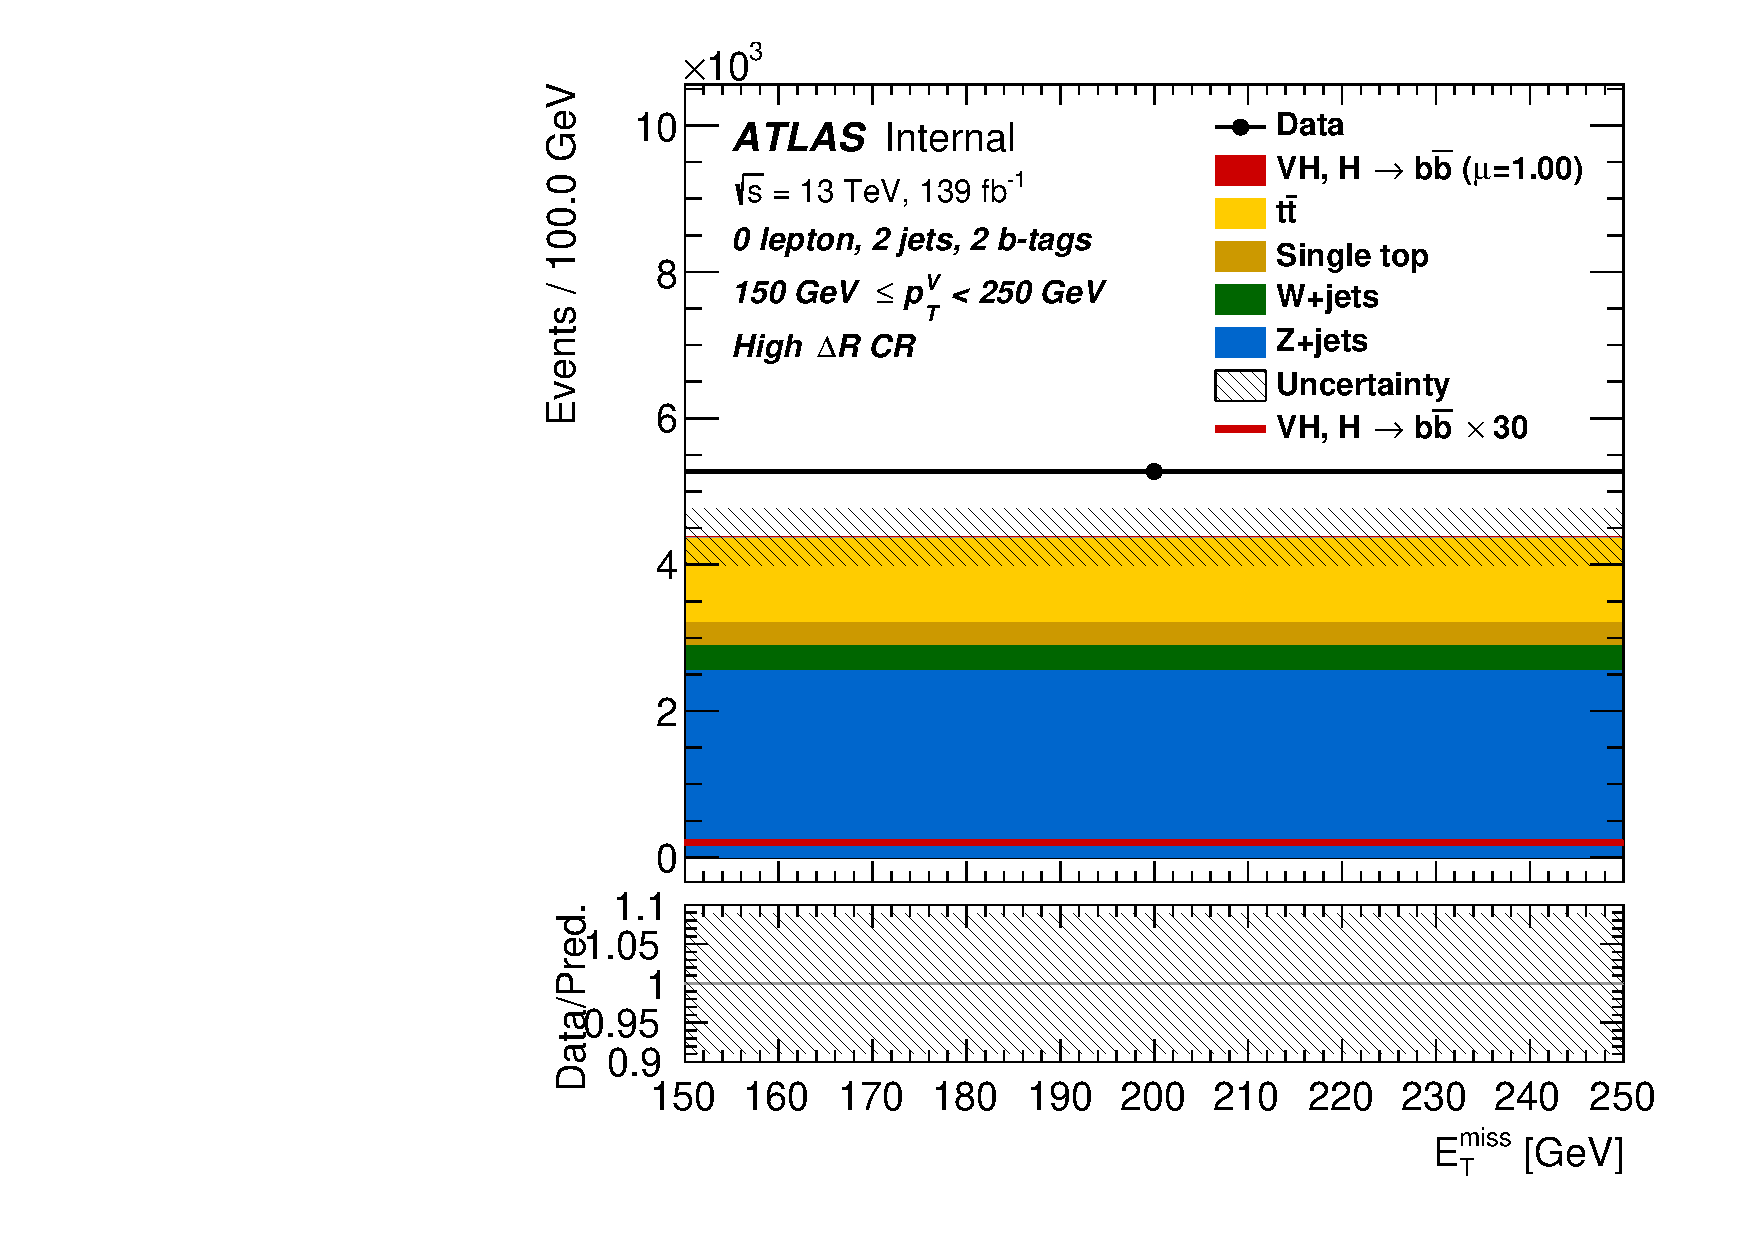
\includegraphics[width=.49\textwidth]{final_fit_mva/prefit/Region_BMax250_BMin150_Y6051_DCRHigh_T2_L0_distMET_J2_Prefit}%
    & 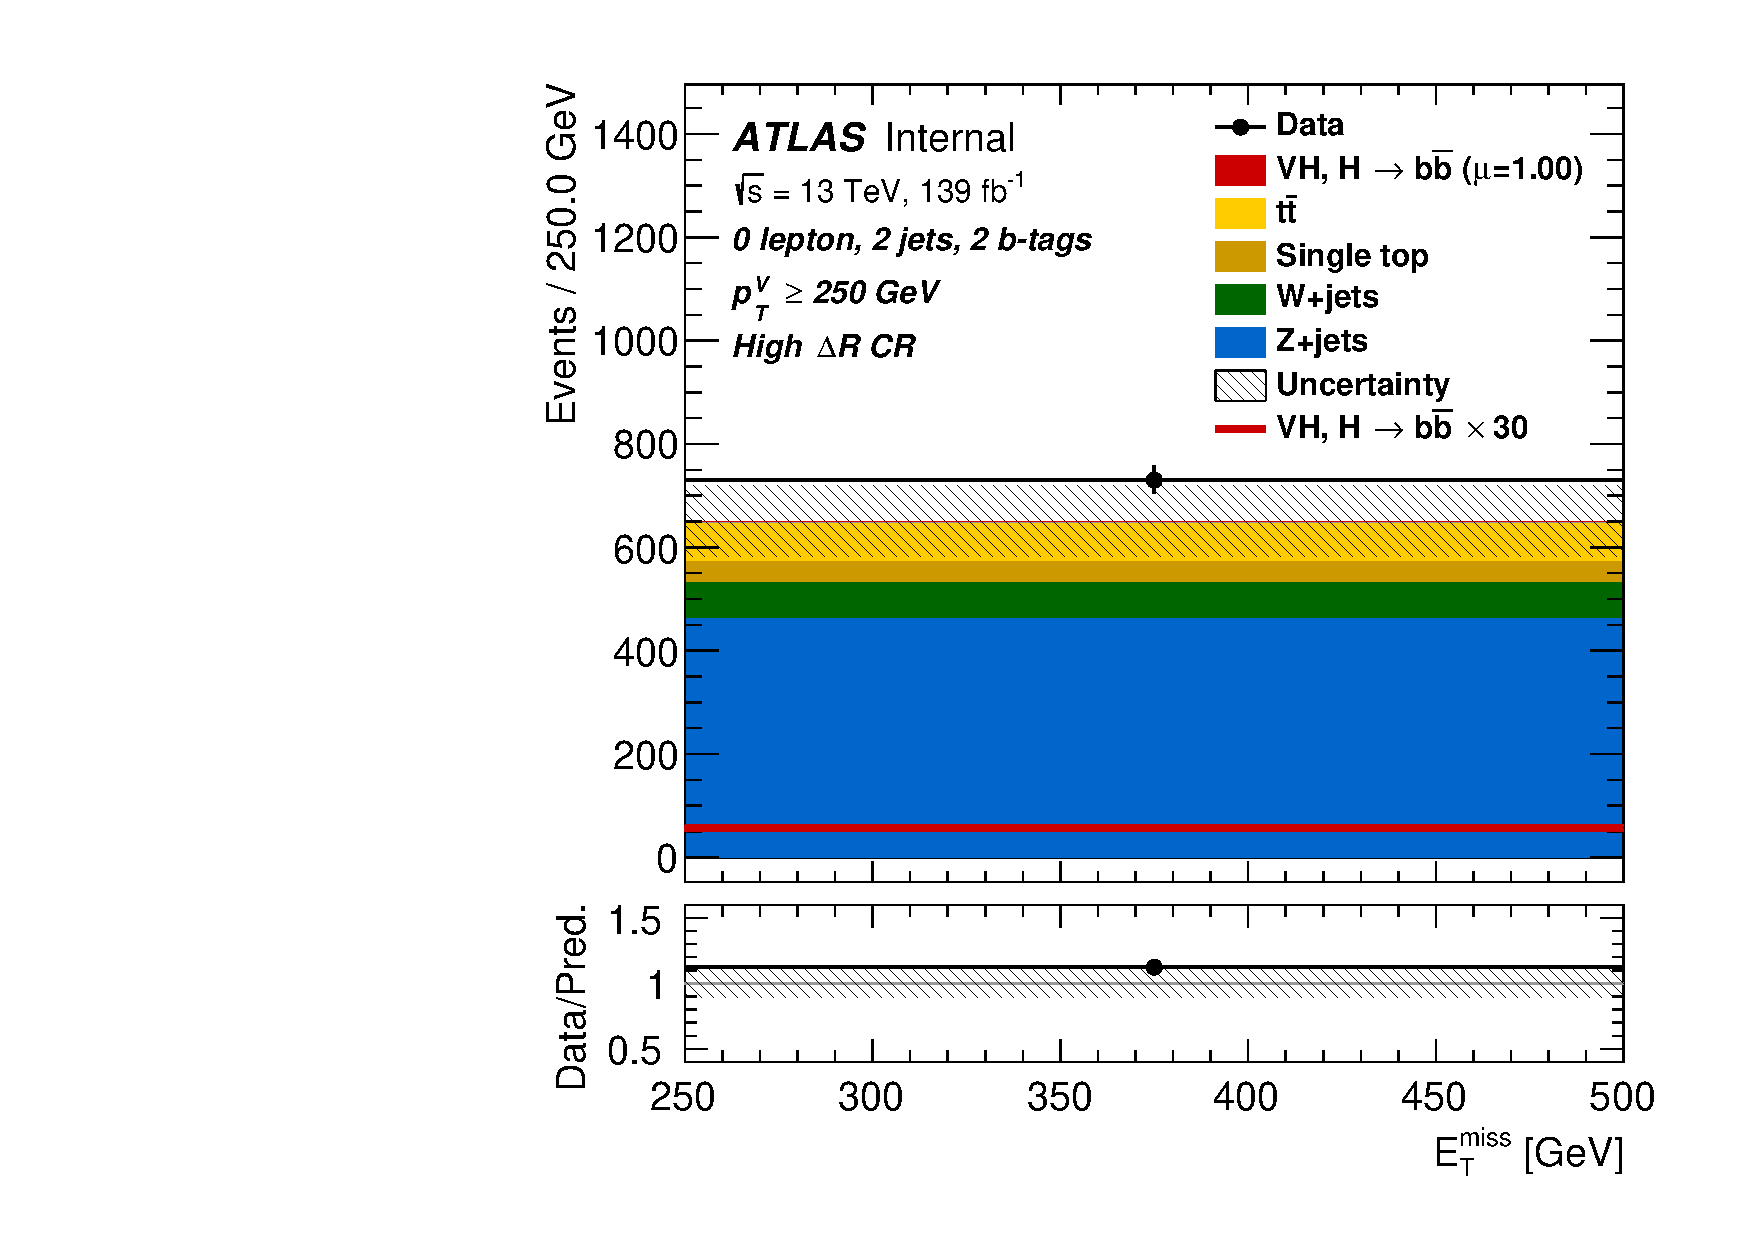
\includegraphics[width=.49\textwidth]{final_fit_mva/prefit/Region_BMin250_Y6051_DCRHigh_T2_L0_distMET_J2_Prefit} \\

    % middle row
    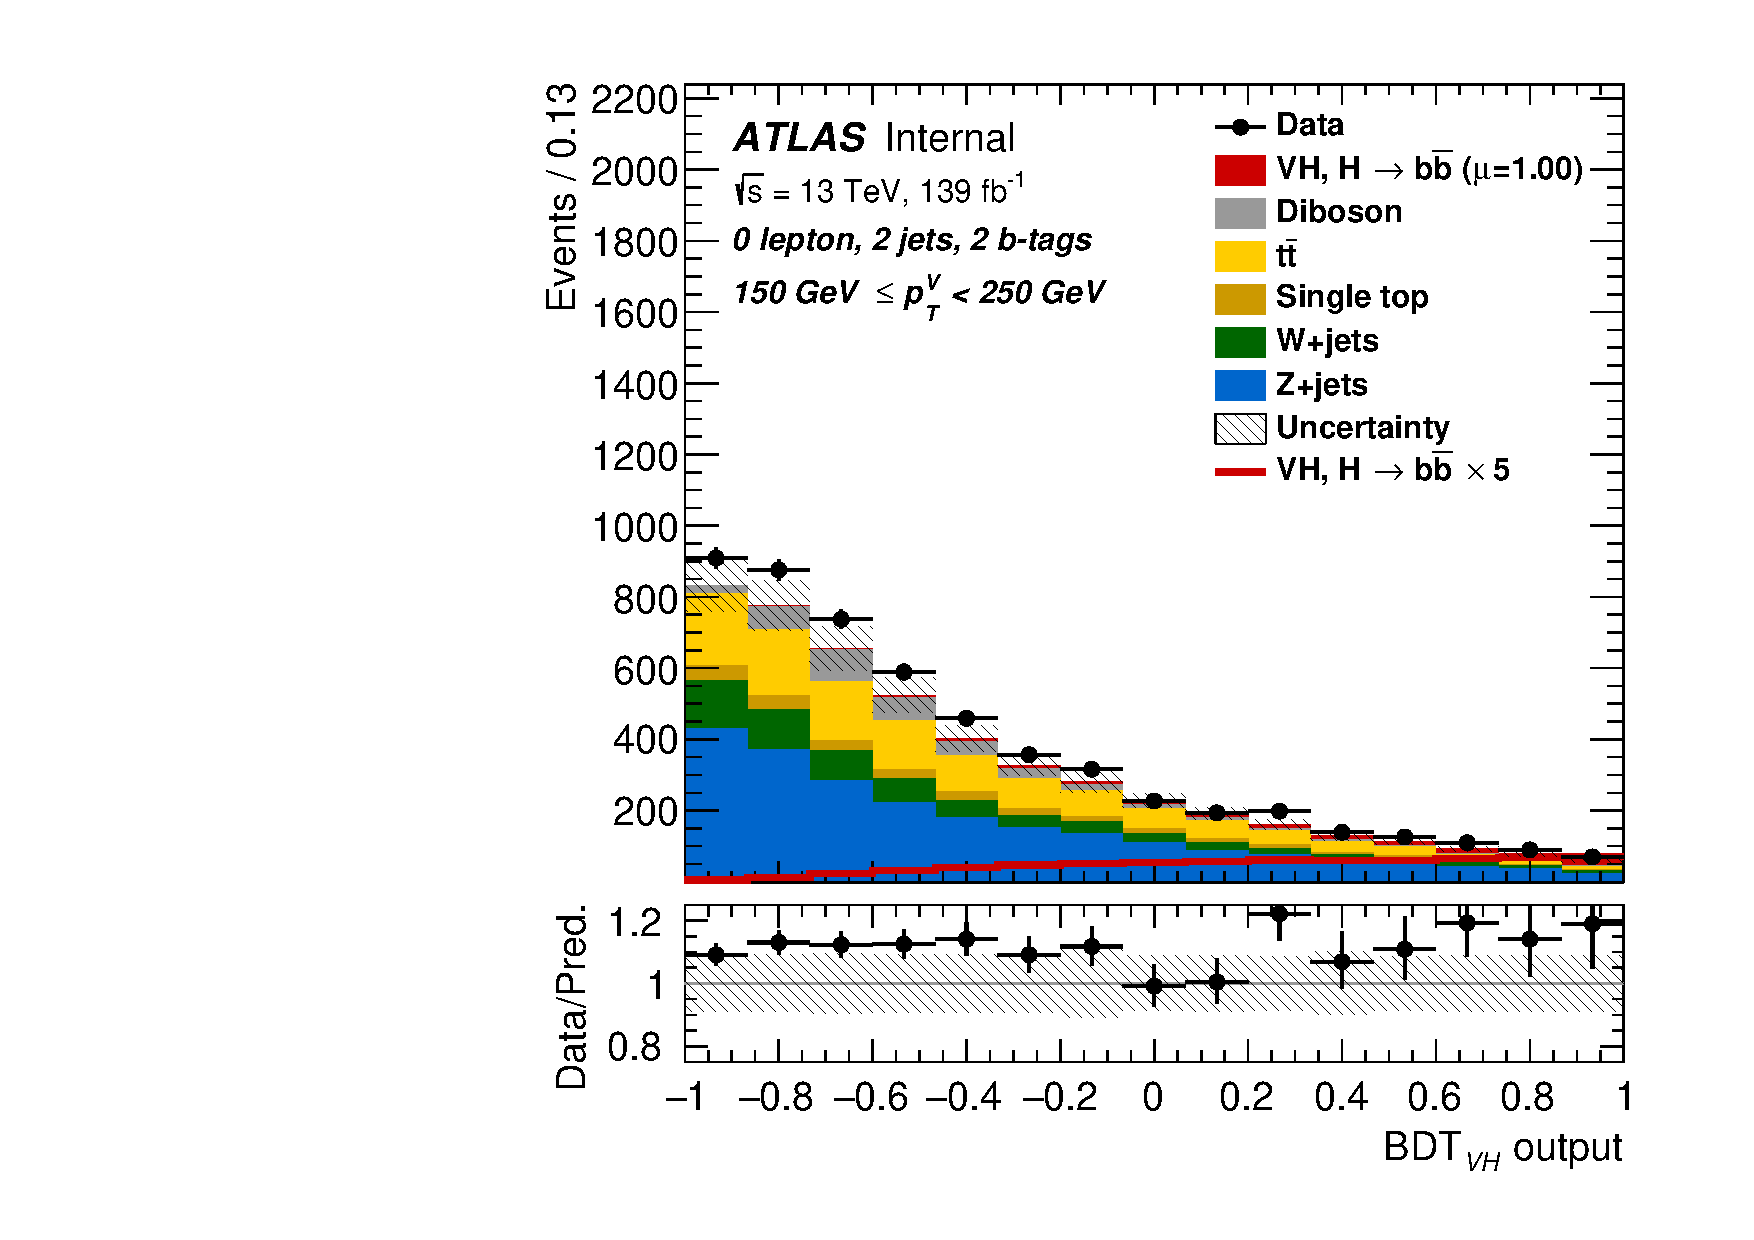
\includegraphics[width=.49\textwidth]{final_fit_mva/prefit/Region_BMax250_BMin150_Y6051_DSR_T2_L0_distmva_J2_Prefit}%
    & 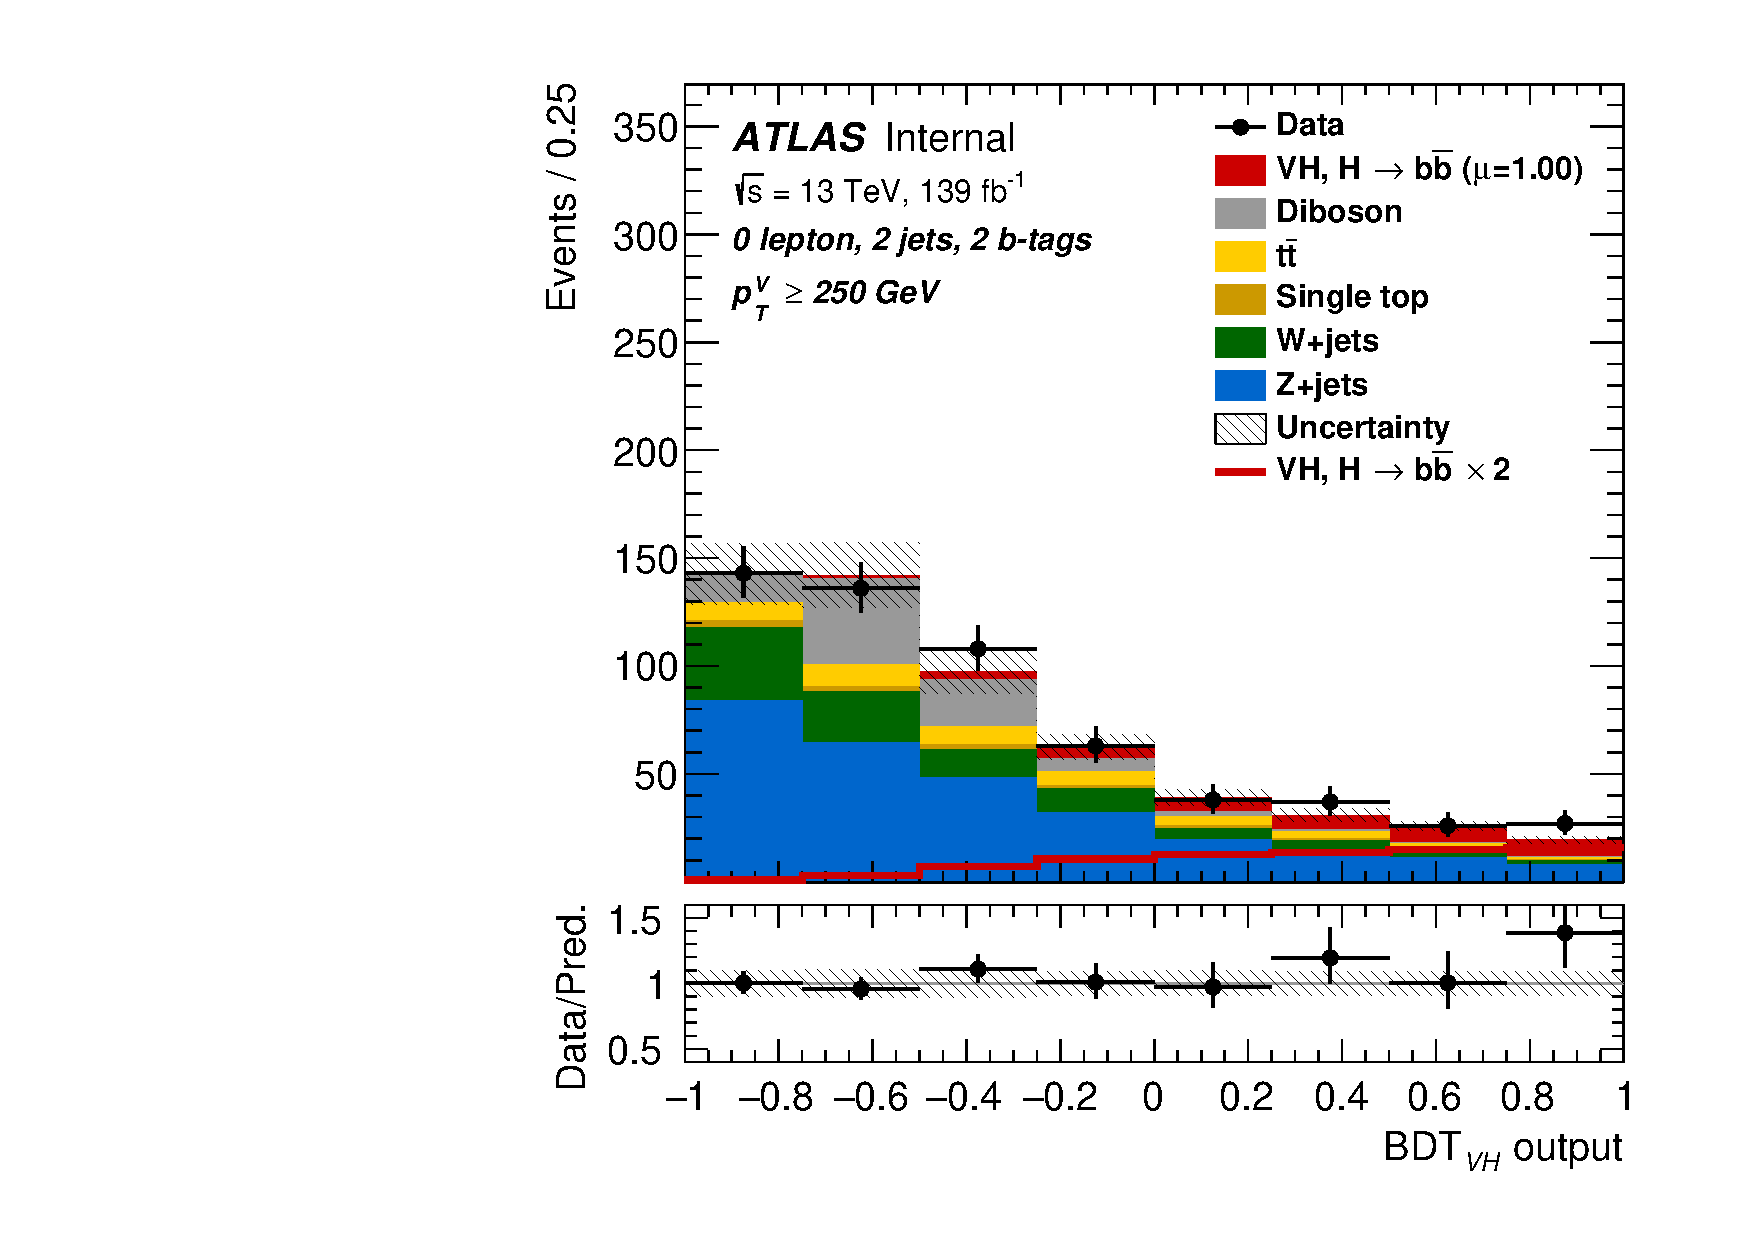
\includegraphics[width=.49\textwidth]{final_fit_mva/prefit/Region_BMin250_Y6051_DSR_T2_L0_distmva_J2_Prefit} \\

    % bottom row
    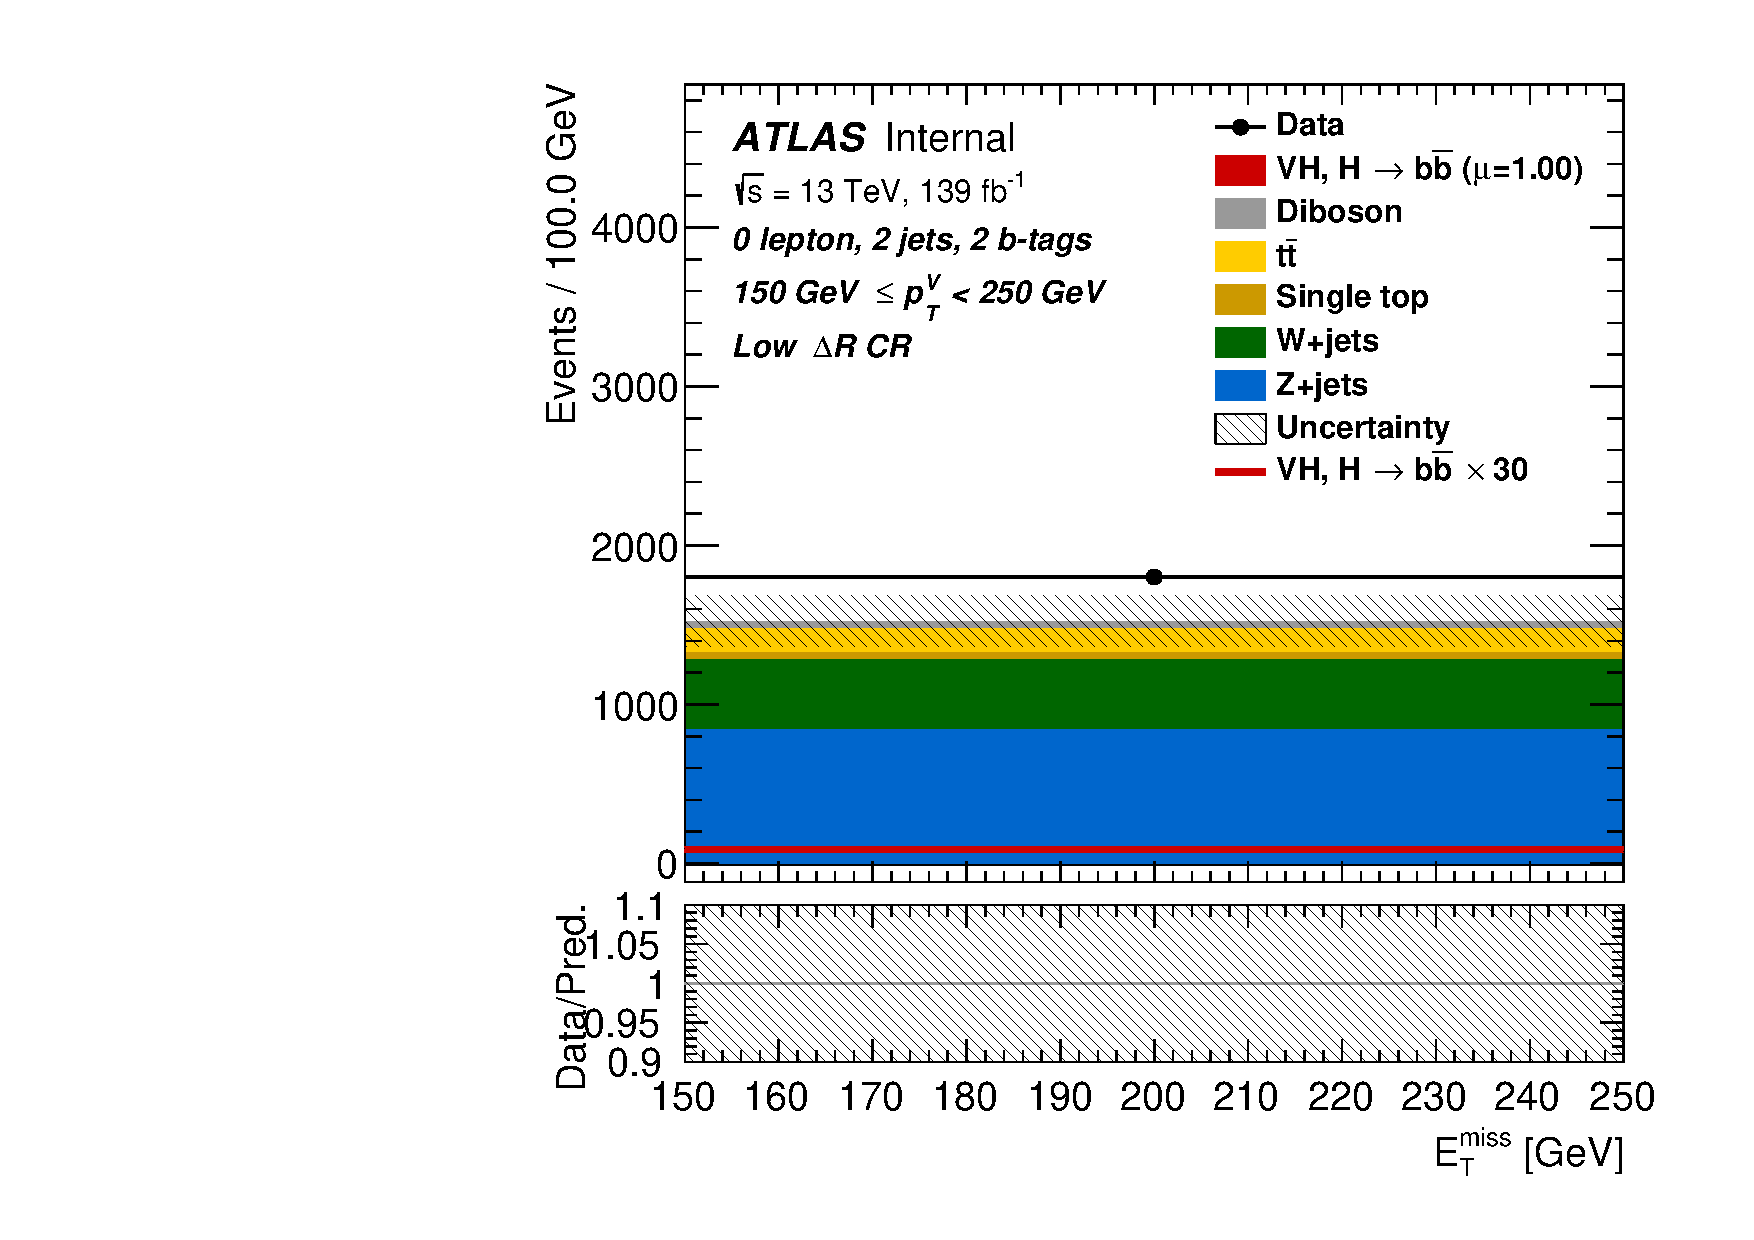
\includegraphics[width=.49\textwidth]{final_fit_mva/prefit/Region_BMax250_BMin150_Y6051_DCRLow_T2_L0_distMET_J2_Prefit}%
    & 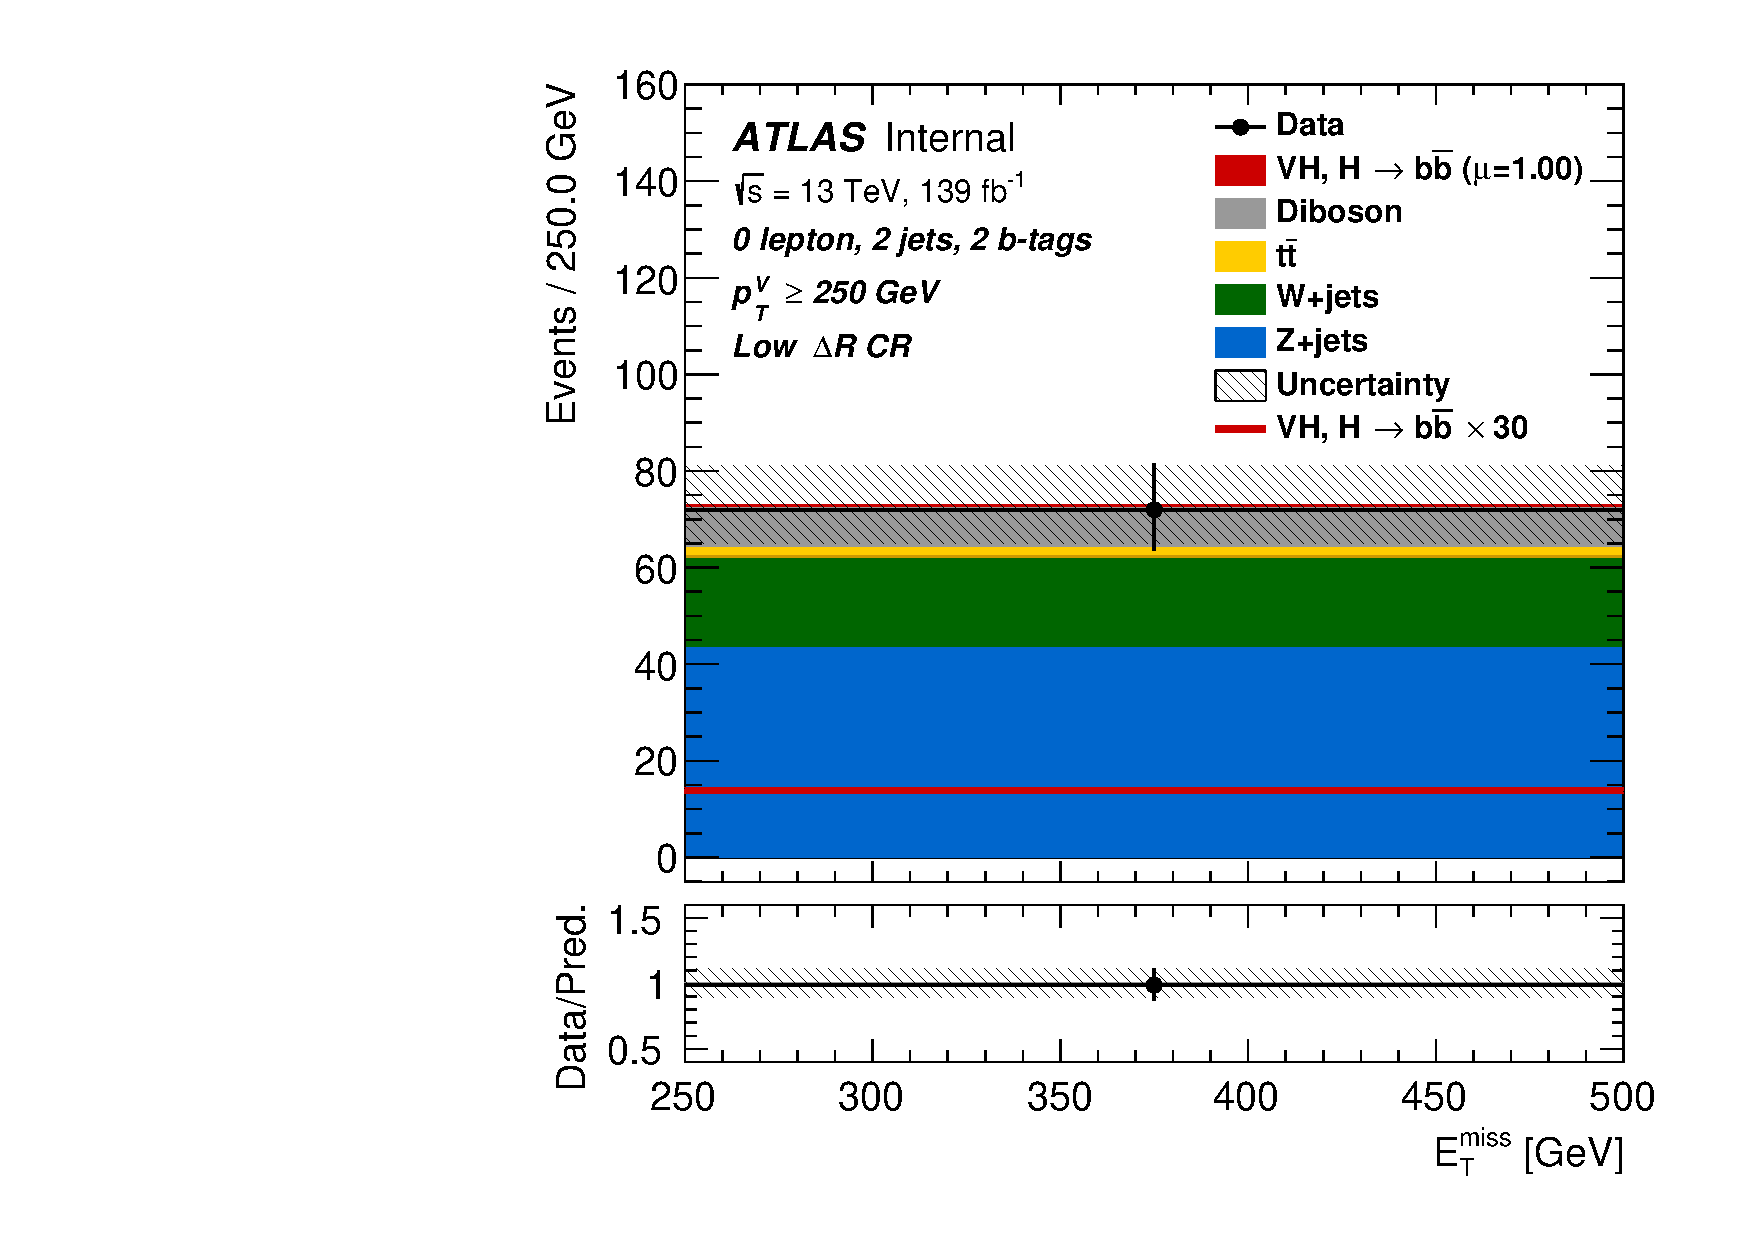
\includegraphics[width=.49\textwidth]{final_fit_mva/prefit/Region_BMin250_Y6051_DCRLow_T2_L0_distMET_J2_Prefit} \\
  \end{tabular}
  \caption{Pre-fit distributions in the 0--lepton channel in the 2--jet region.}
  \label{fig:0lep-2jet-prefit}
\end{figure}
\begin{figure}
  \centering
  \begin{tabular}{cc}
    % top row
    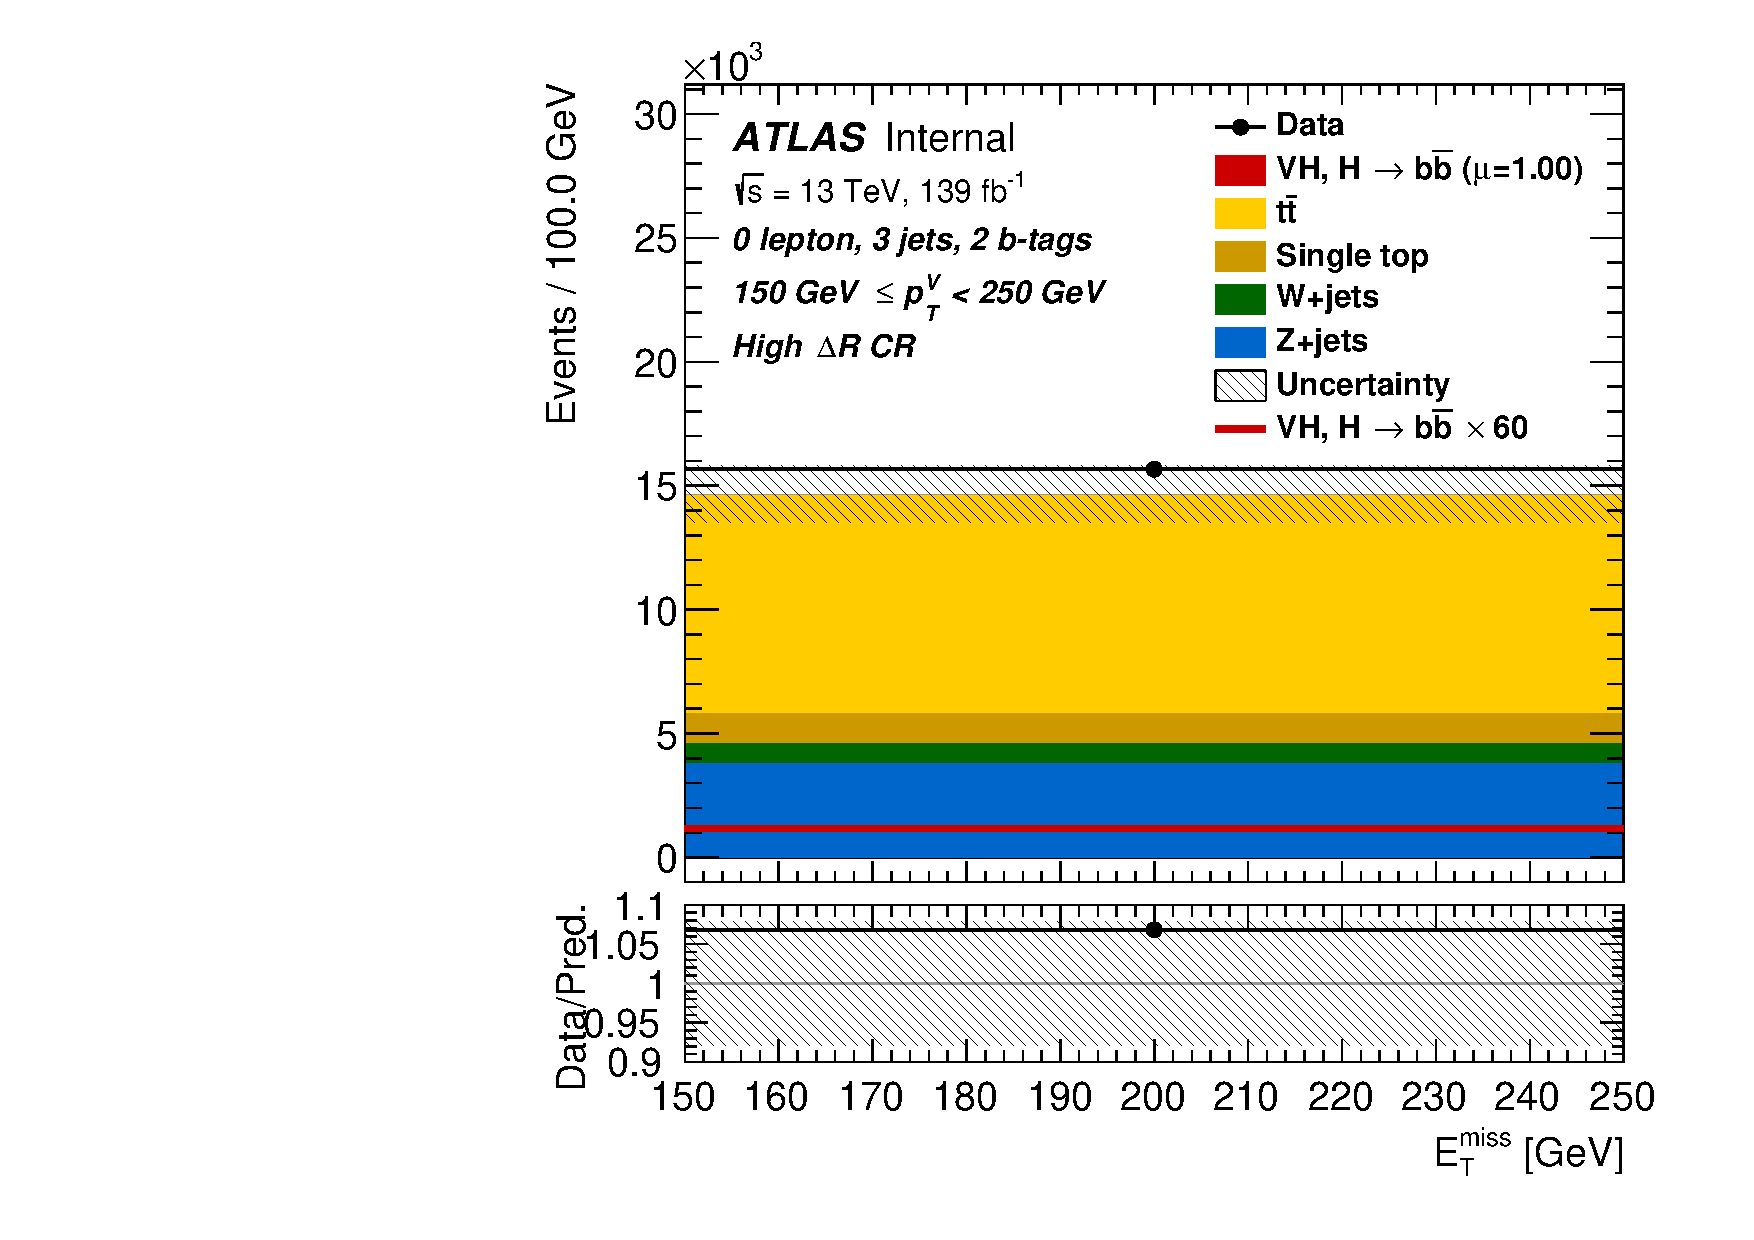
\includegraphics[width=.3\textwidth]{final_fit_mva/prefit/Region_BMax250_BMin150_Y6051_DCRHigh_T2_L0_distMET_J3_Prefit}%
    & 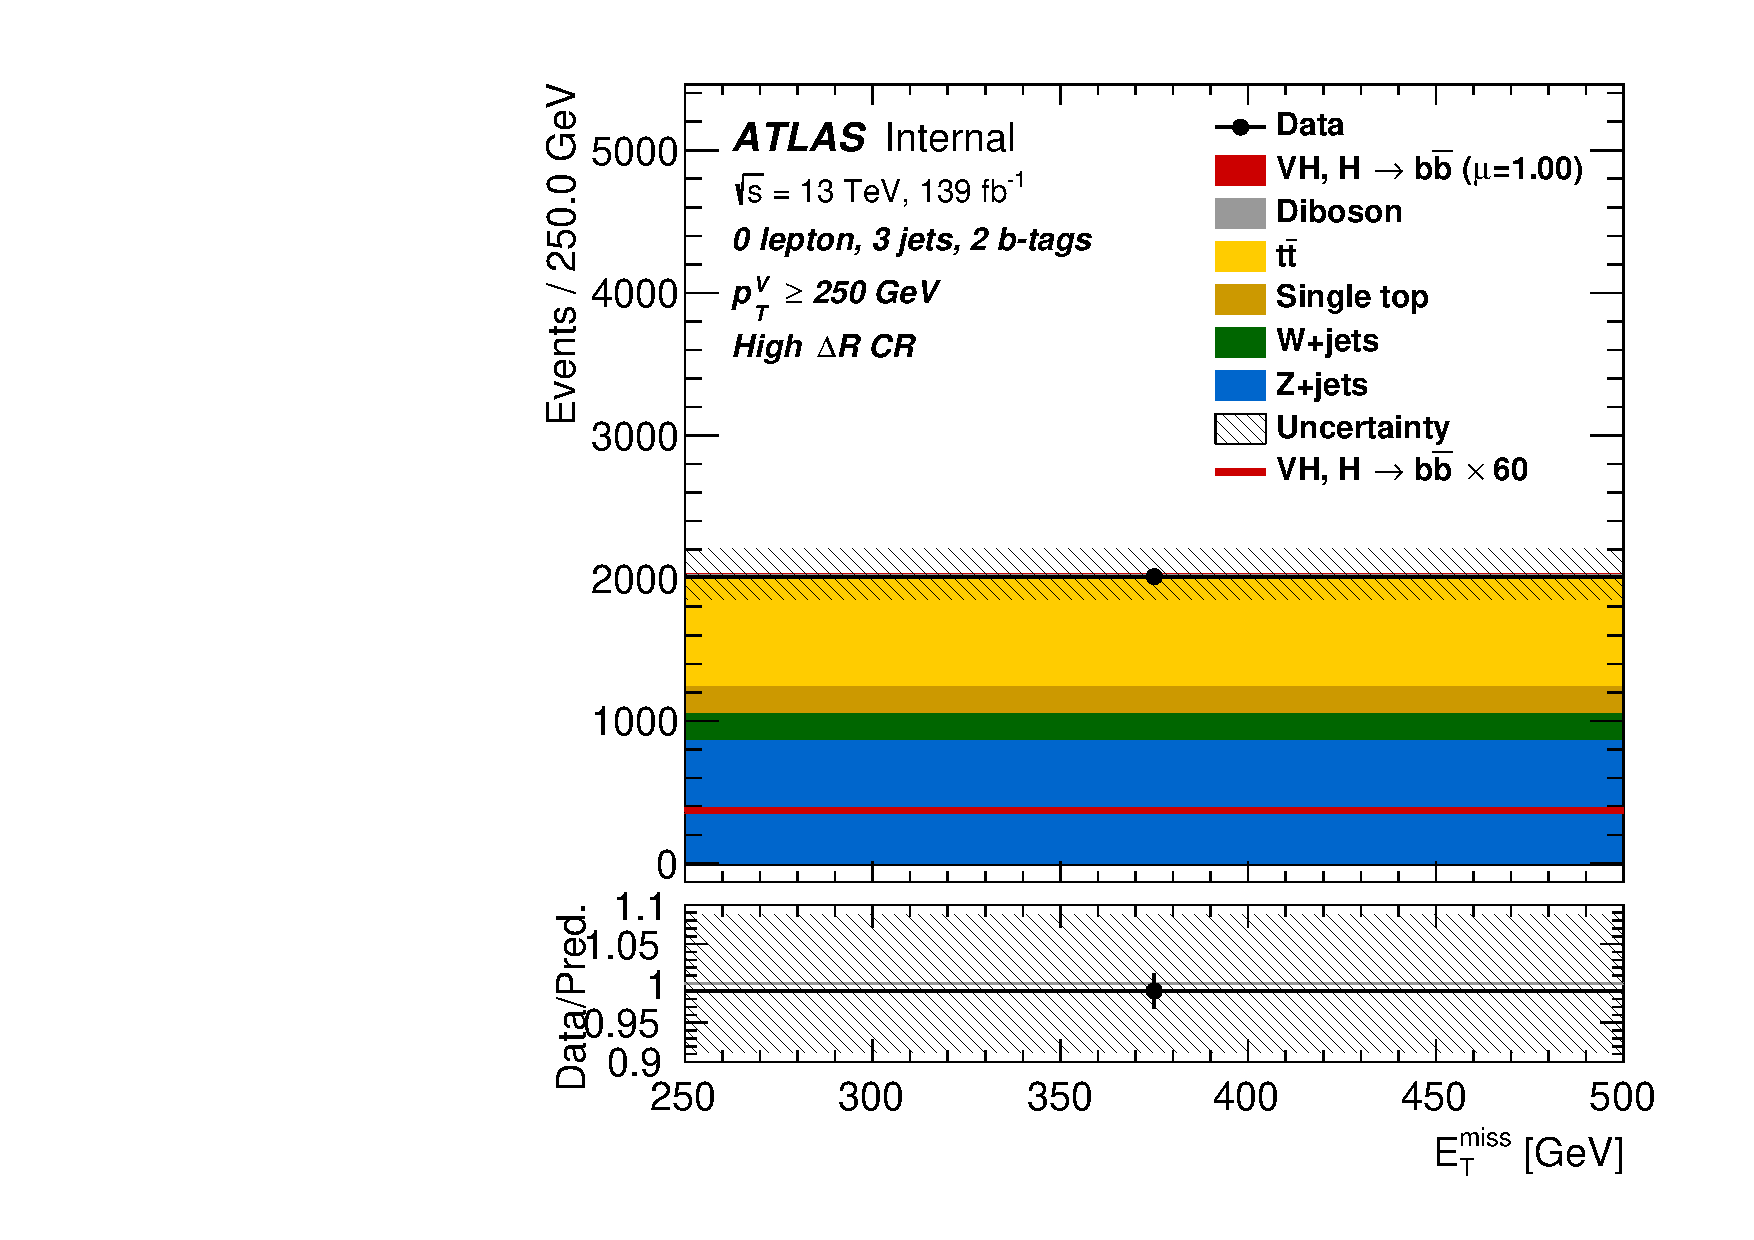
\includegraphics[width=.3\textwidth]{final_fit_mva/prefit/Region_BMin250_Y6051_DCRHigh_T2_L0_distMET_J3_Prefit} \\

    % middle row
    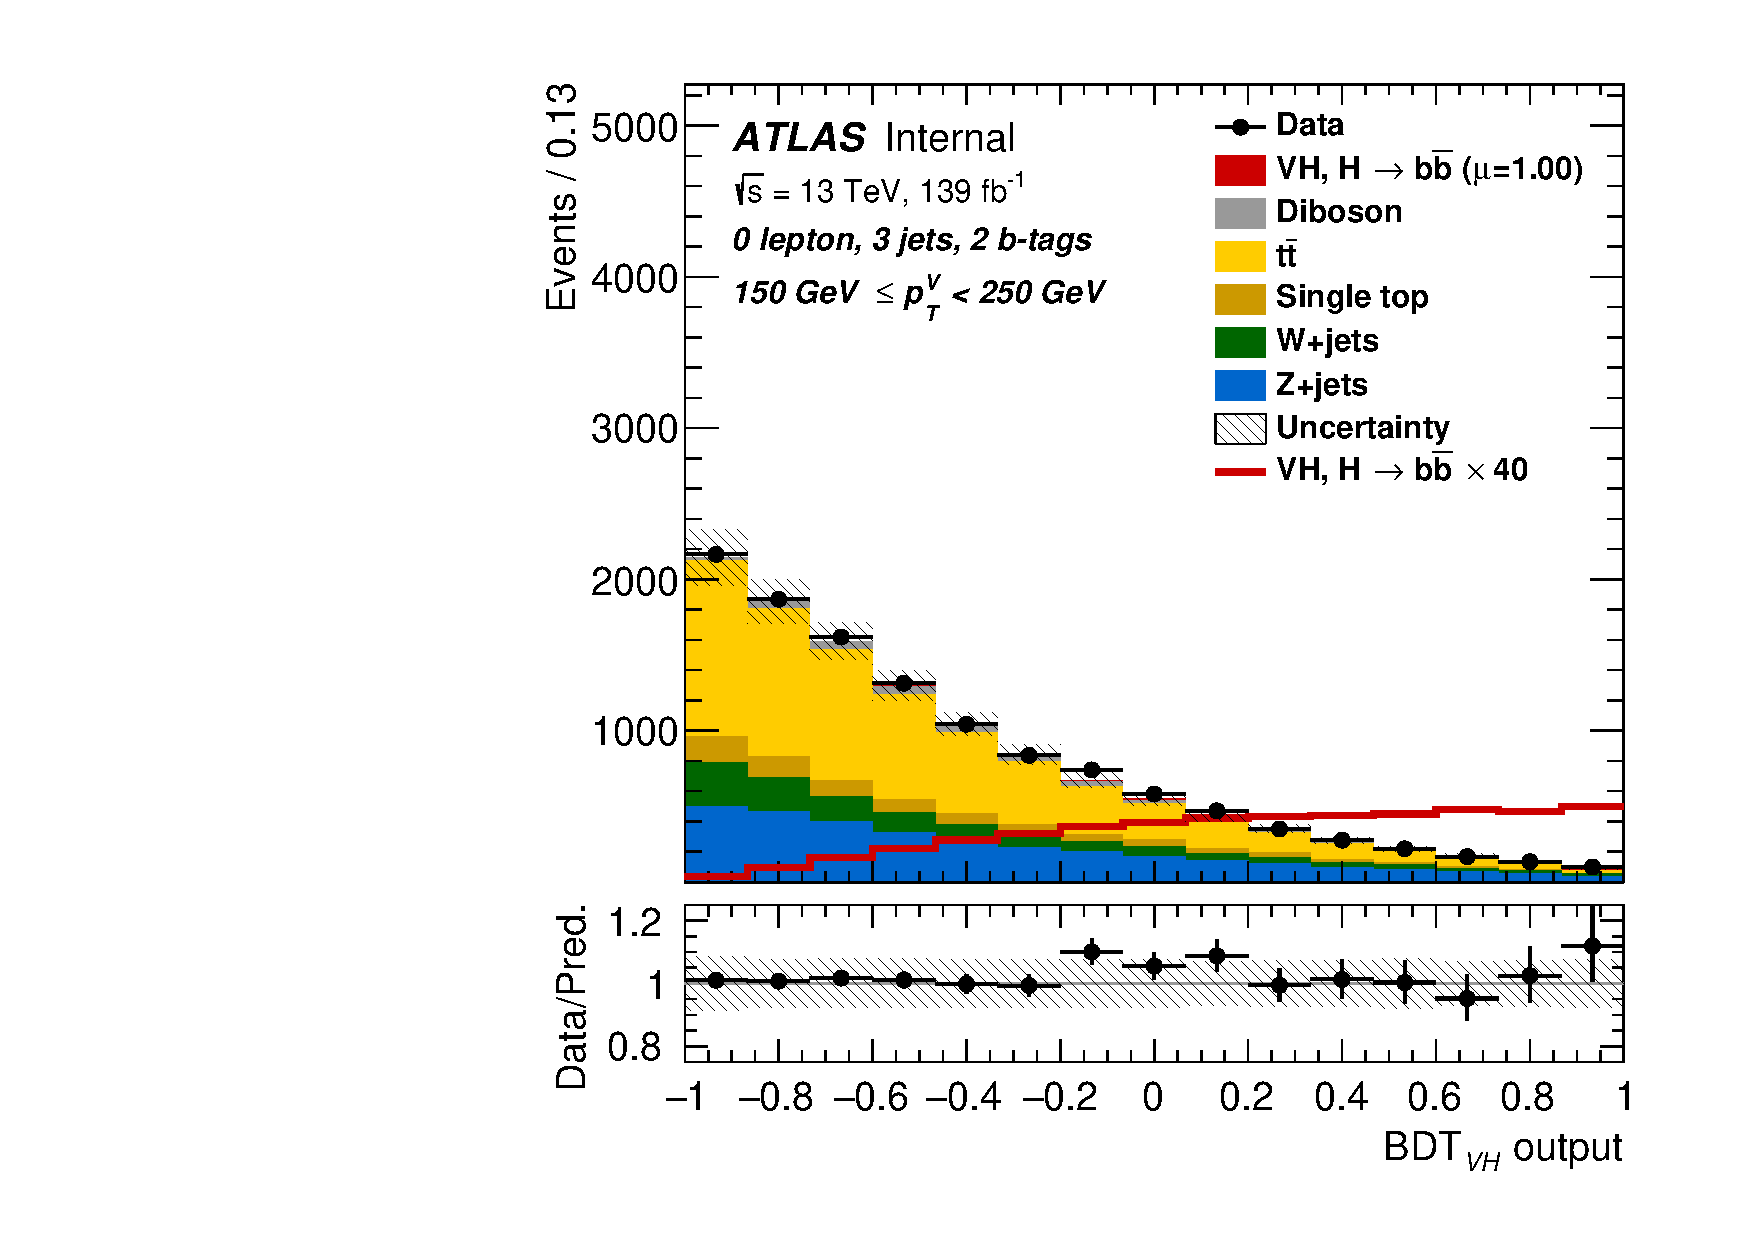
\includegraphics[width=.3\textwidth]{final_fit_mva/prefit/Region_BMax250_BMin150_Y6051_DSR_T2_L0_distmva_J3_Prefit}%
    & 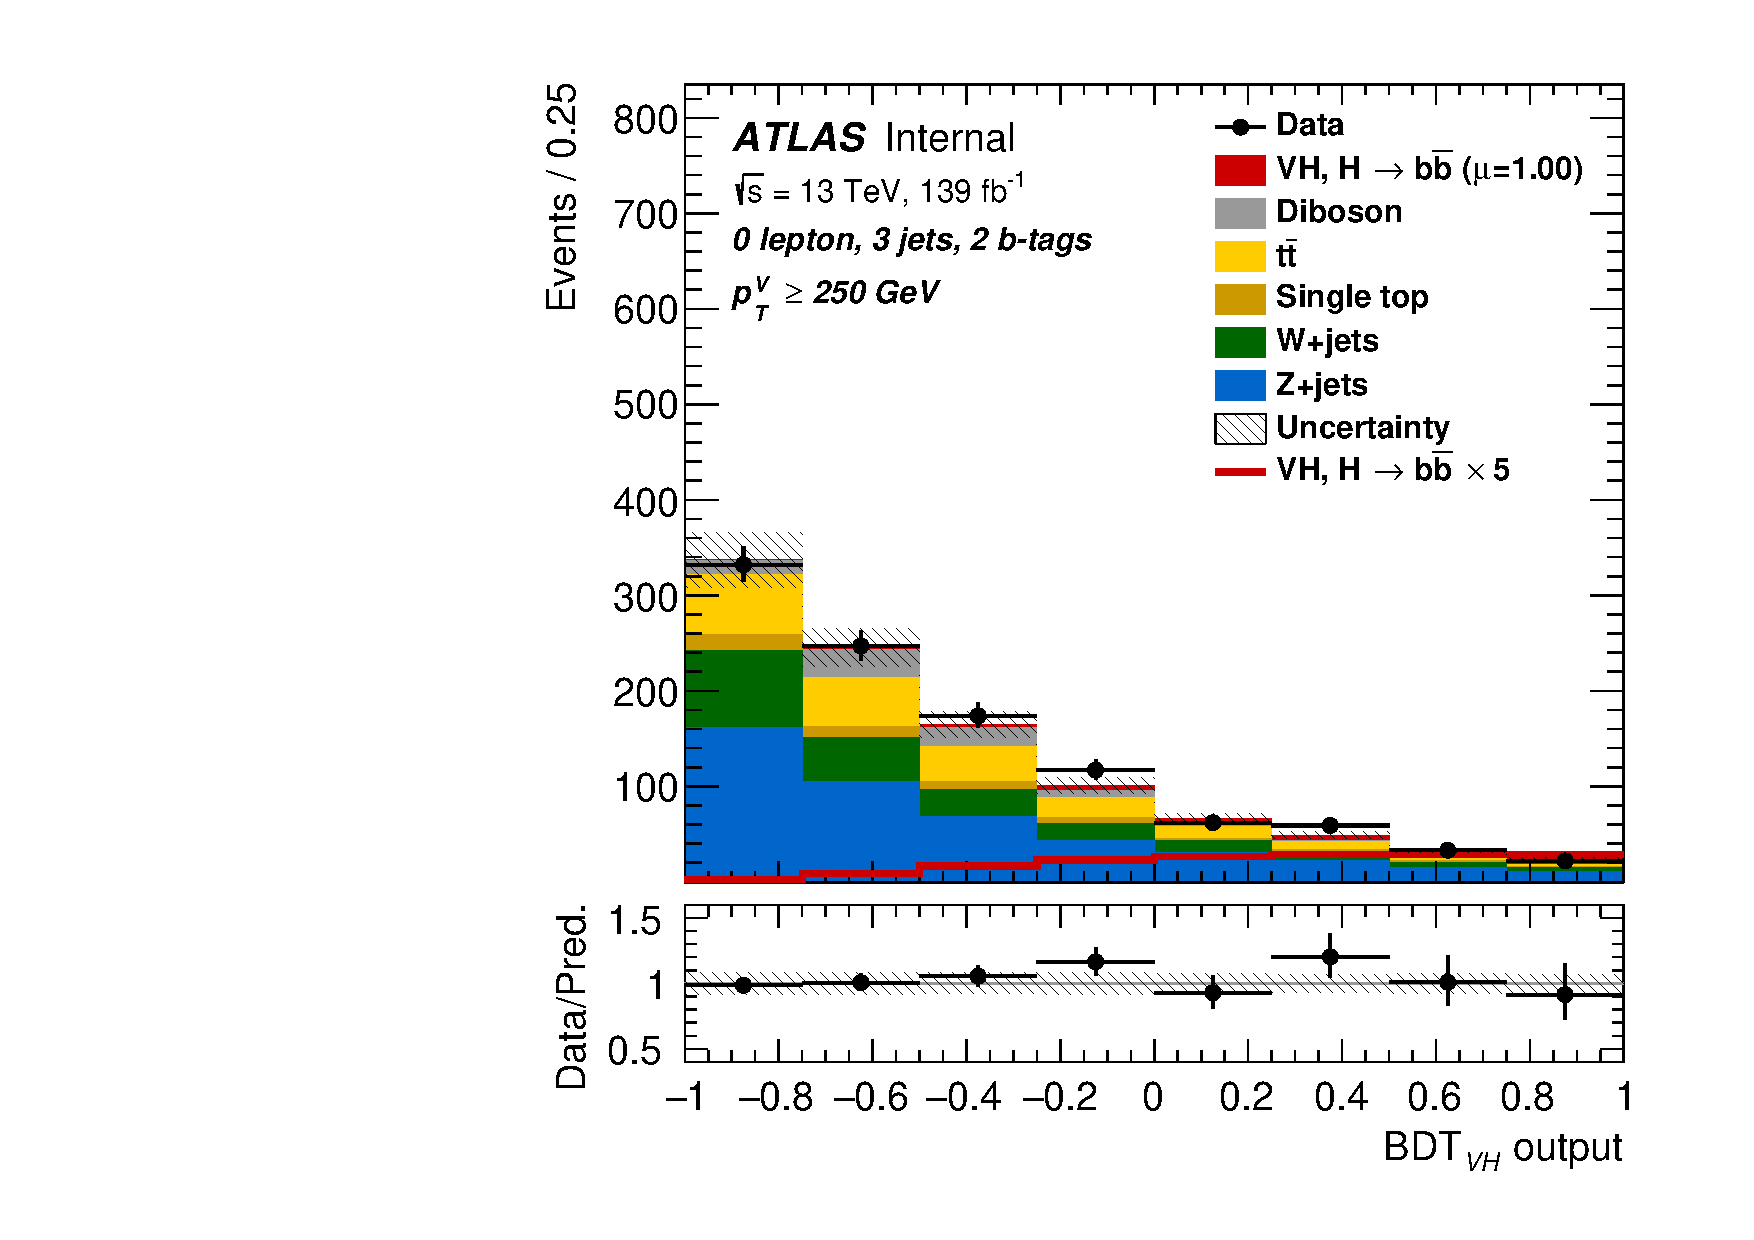
\includegraphics[width=.3\textwidth]{final_fit_mva/prefit/Region_BMin250_Y6051_DSR_T2_L0_distmva_J3_Prefit} \\

    % bottom row
    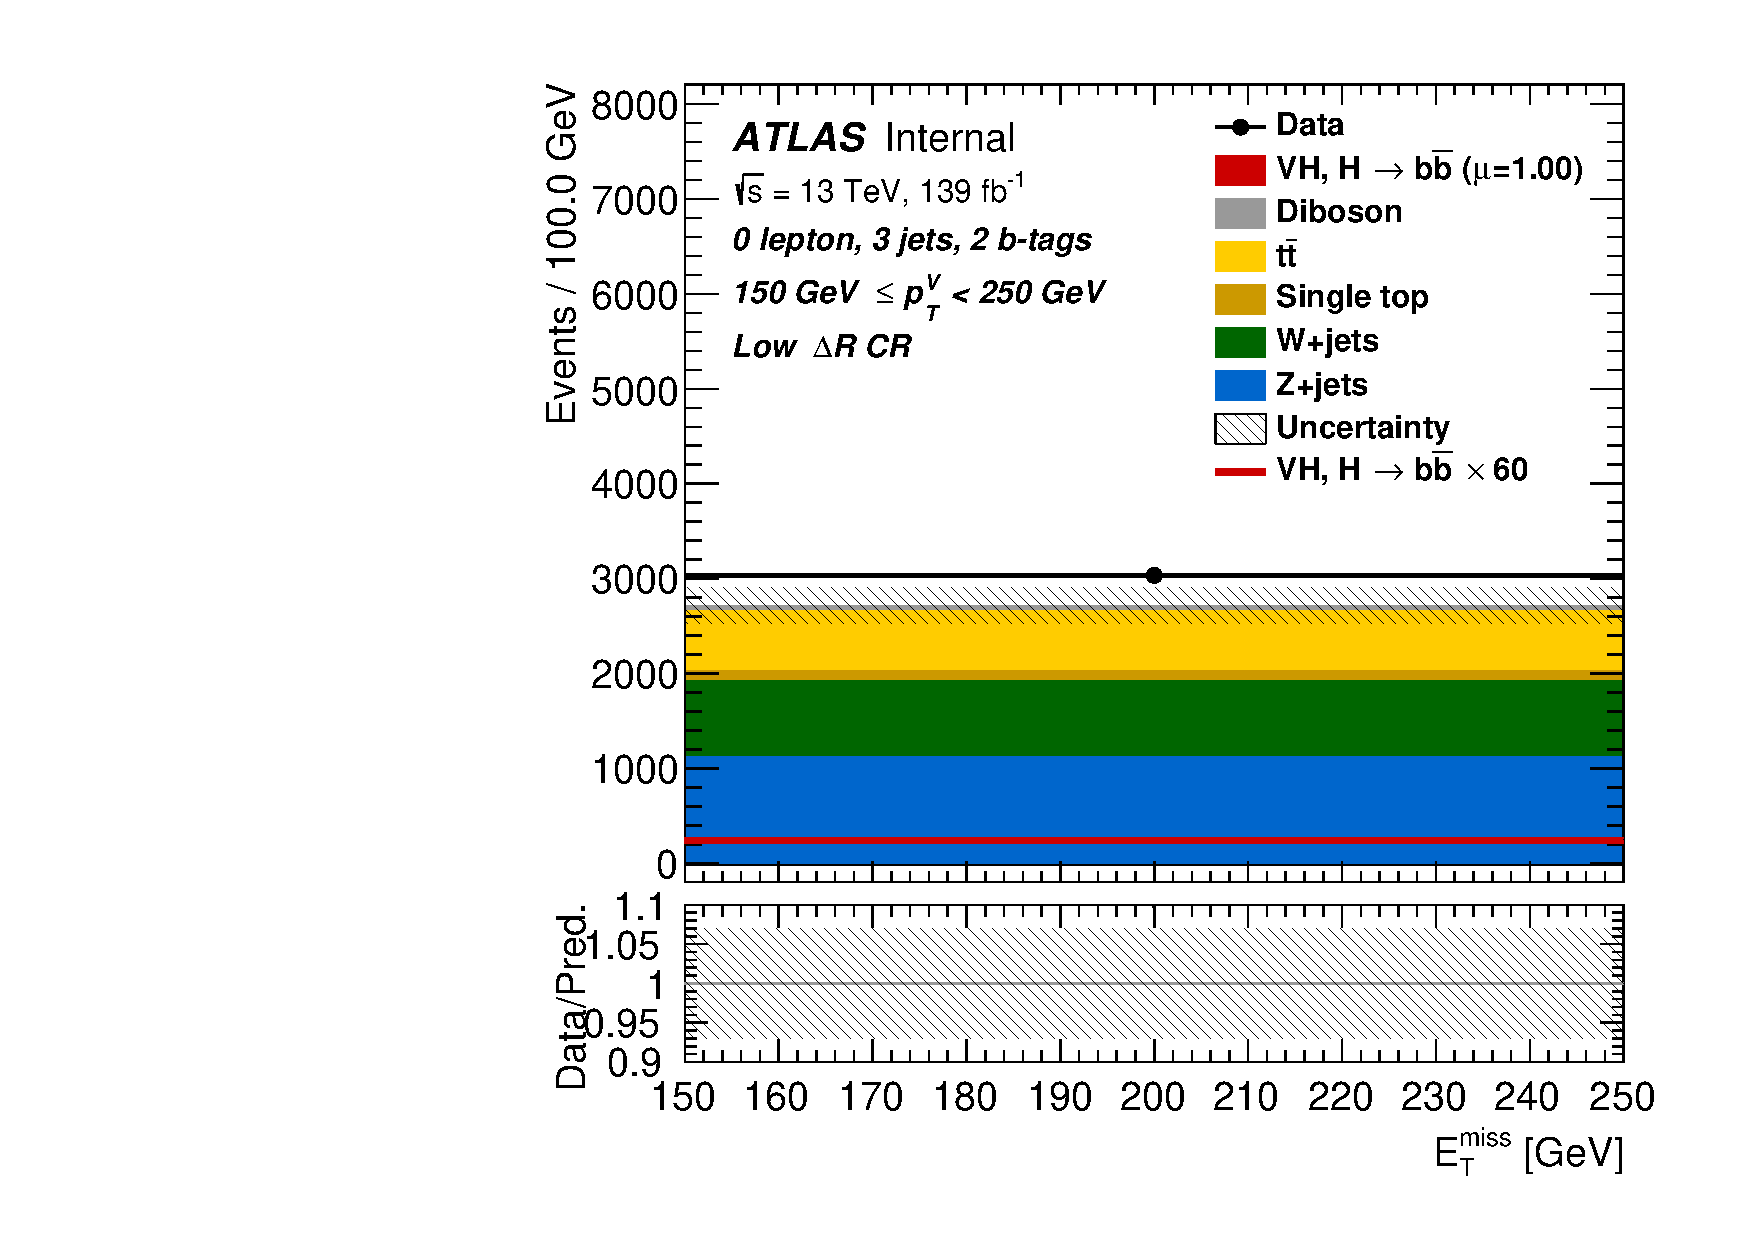
\includegraphics[width=.3\textwidth]{final_fit_mva/prefit/Region_BMax250_BMin150_Y6051_DCRLow_T2_L0_distMET_J3_Prefit}%
    & 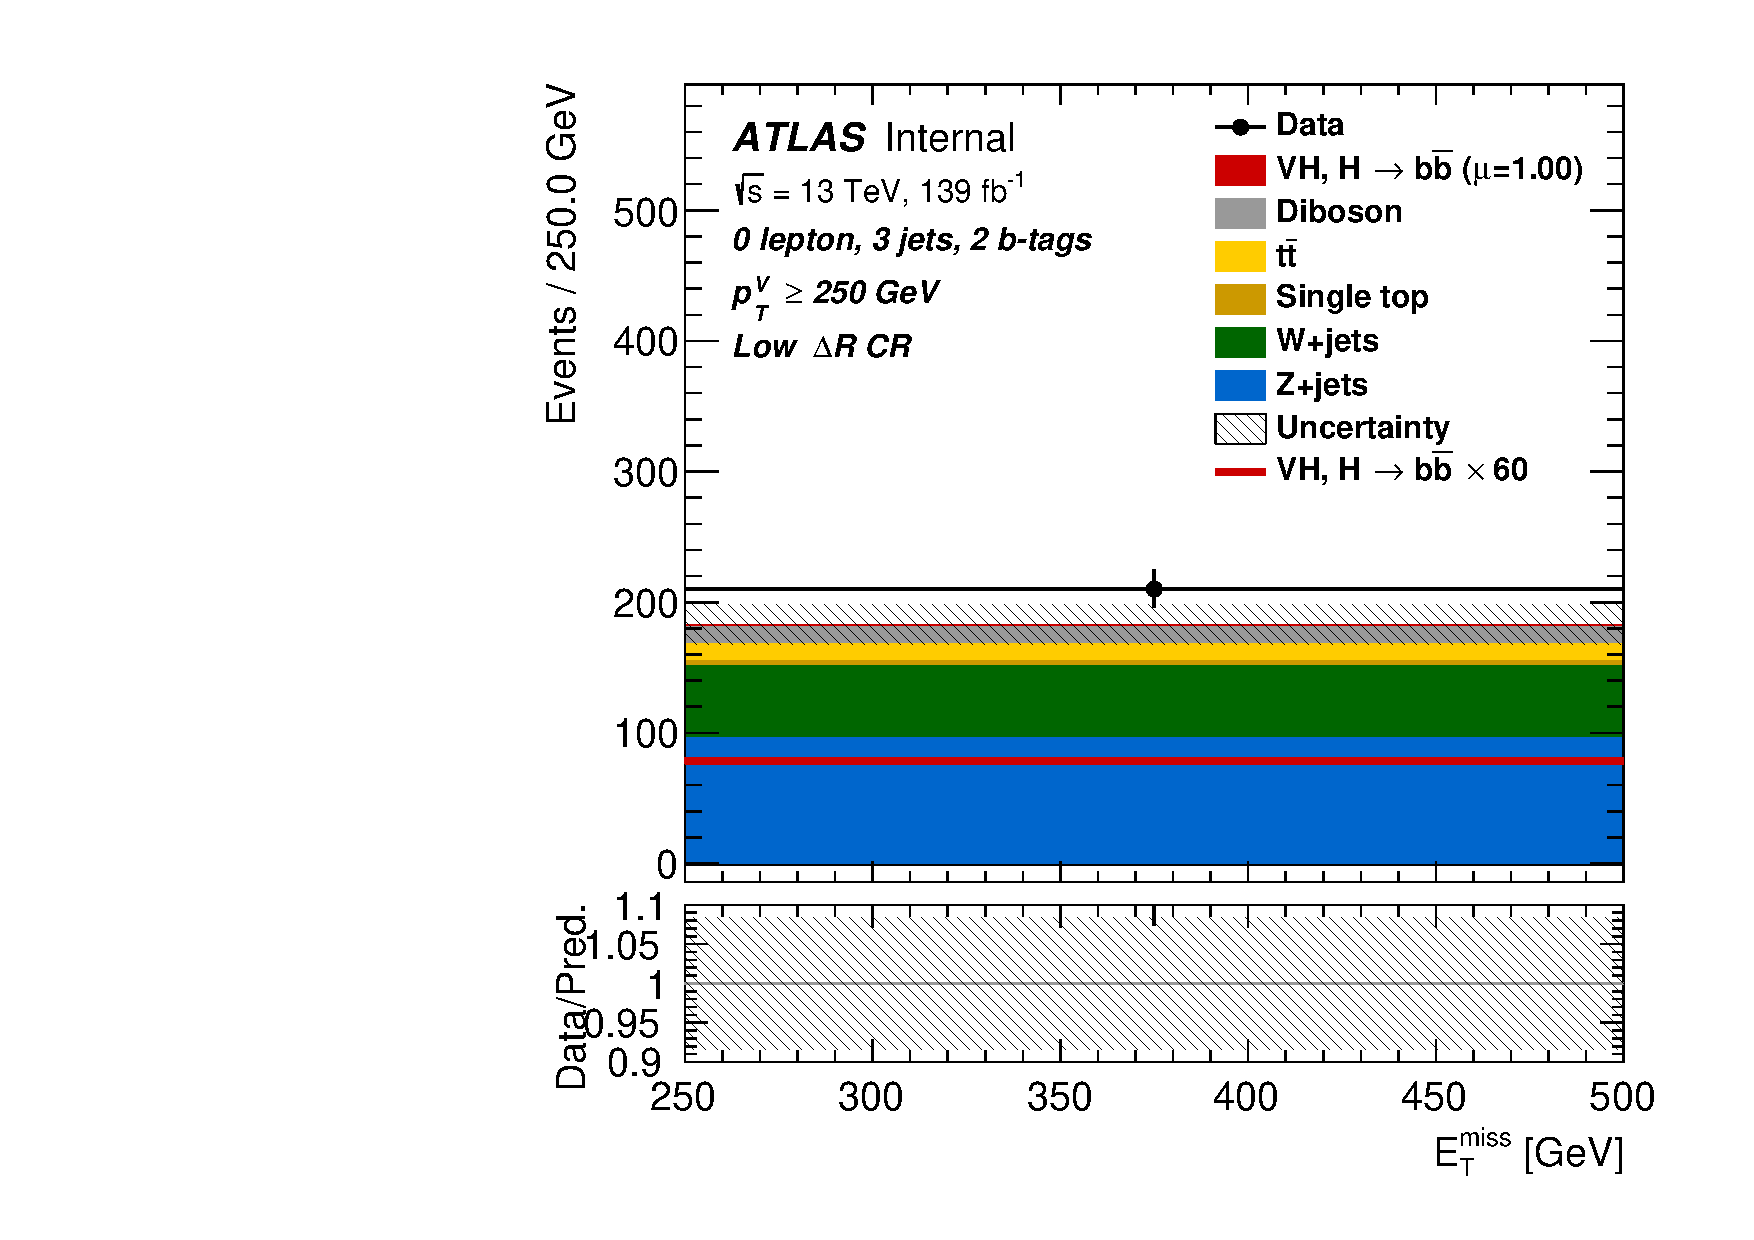
\includegraphics[width=.3\textwidth]{final_fit_mva/prefit/Region_BMin250_Y6051_DCRLow_T2_L0_distMET_J3_Prefit} \\
  \end{tabular}
  \caption{Pre-fit distributions in the 0 lepton 3 jet channel.}
\end{figure}
\begin{figure}
  \centering
  \begin{tabular}{cc}
    % top row
    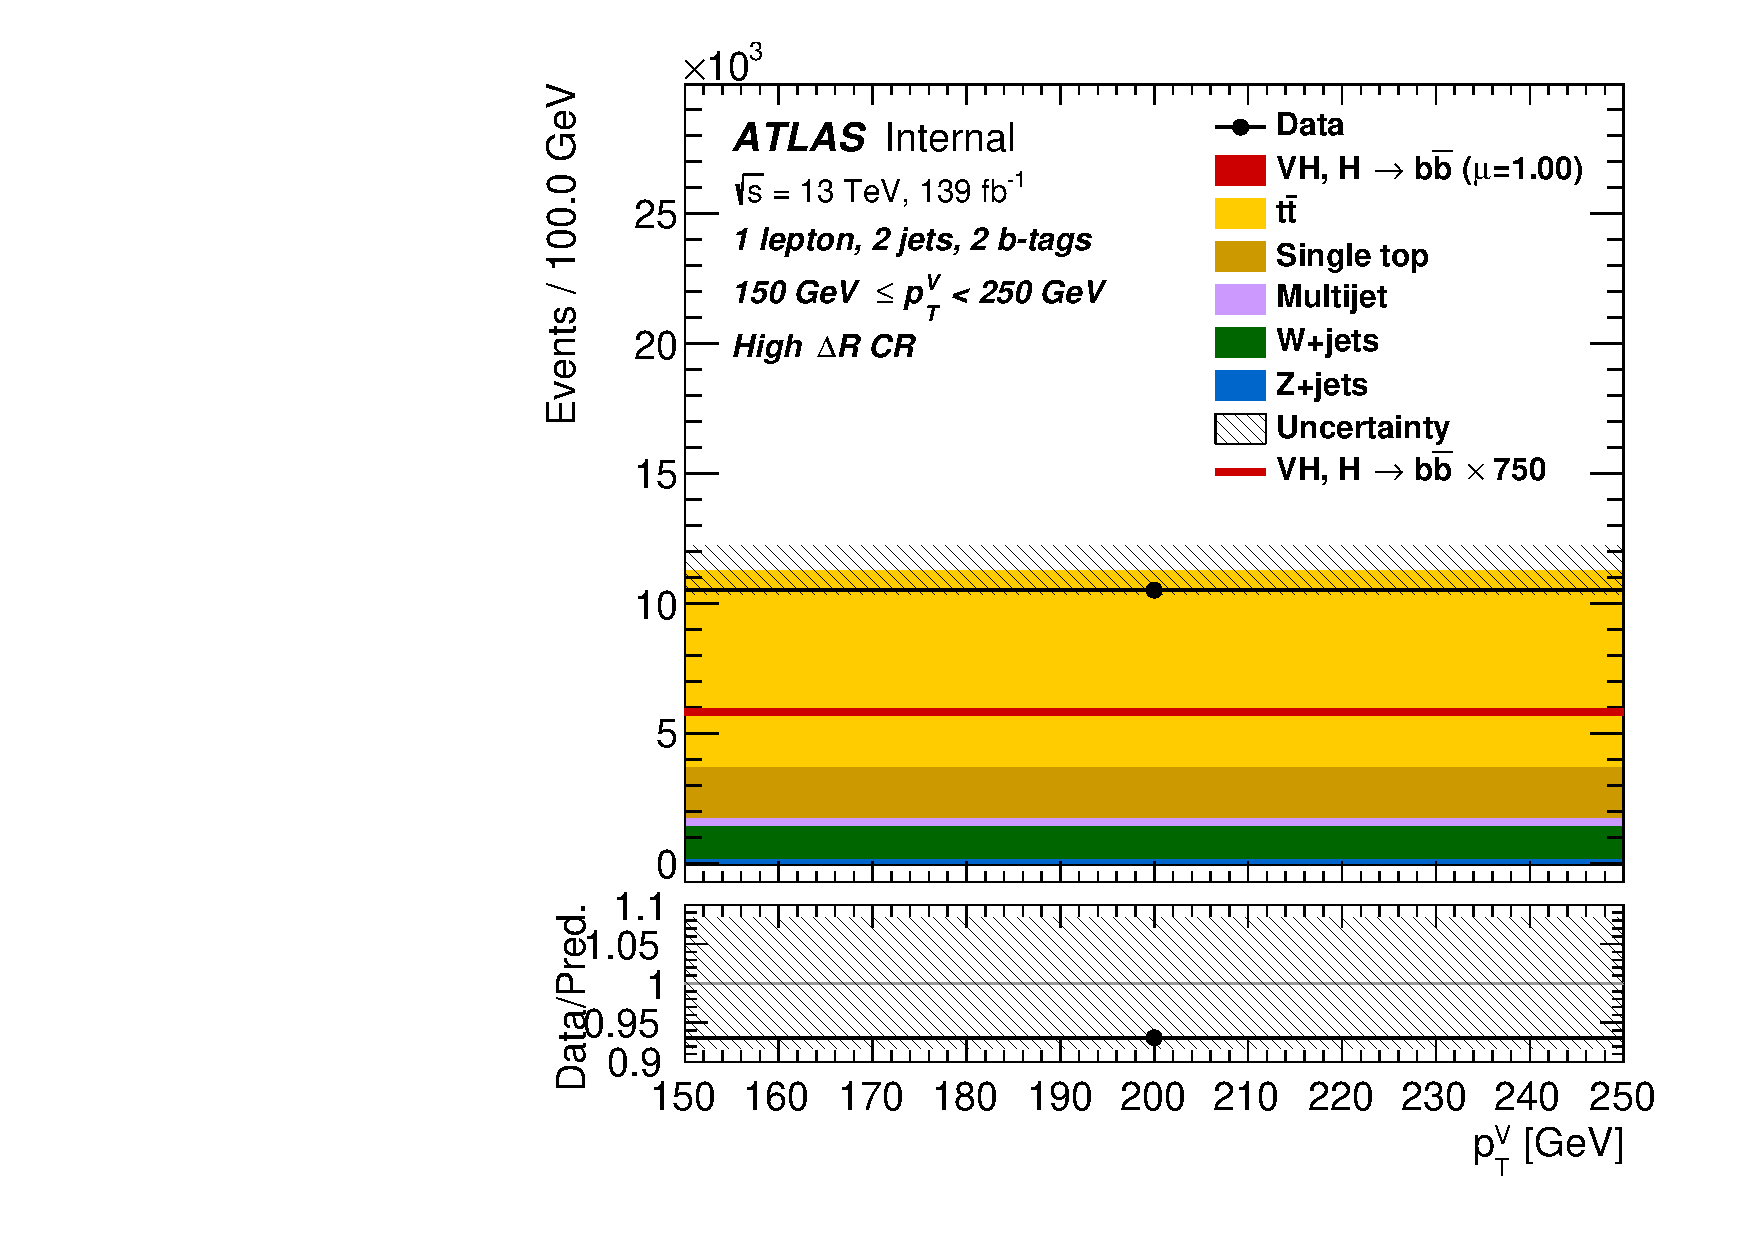
\includegraphics[width=.3\textwidth]{final_fit_mva/prefit/Region_BMax250_BMin150_Y6051_DCRHigh_T2_L1_distpTV_J2_Prefit}%
    & 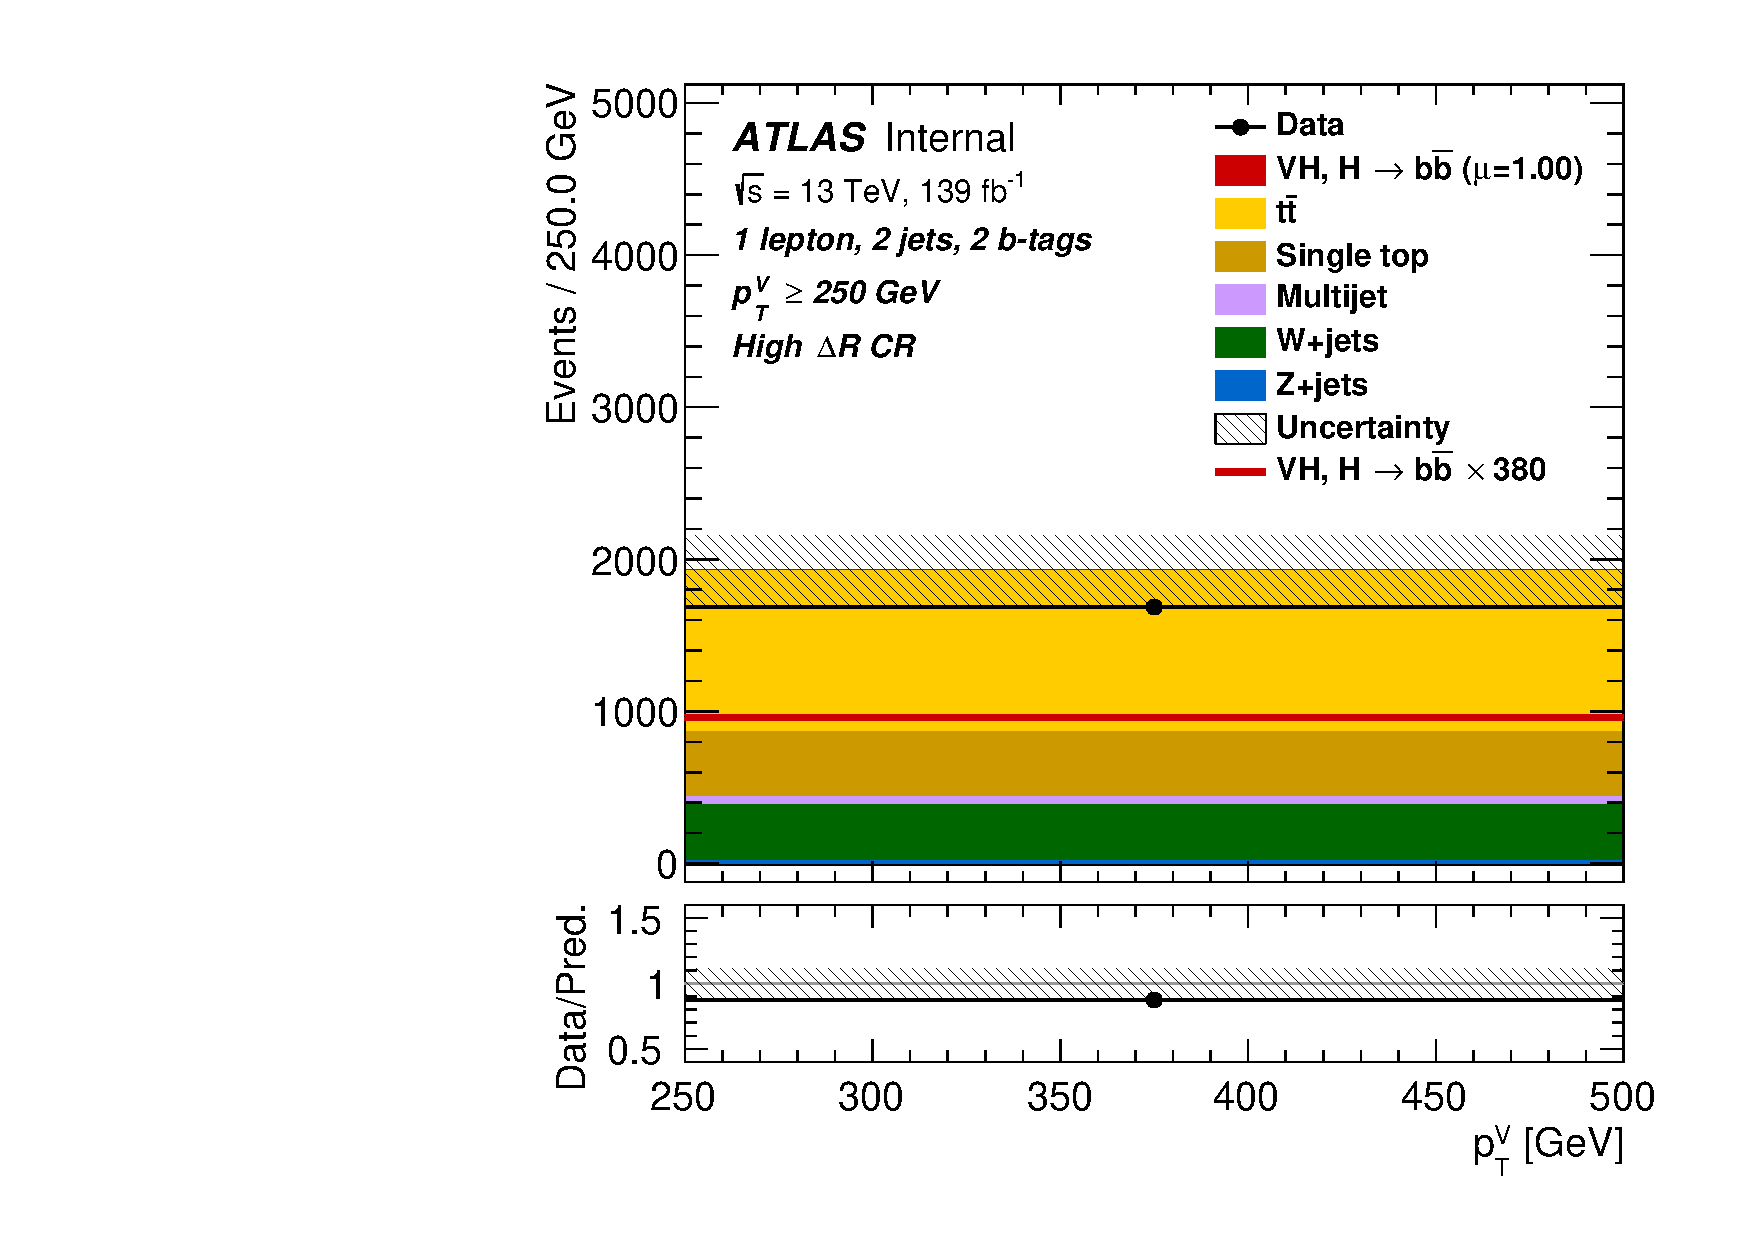
\includegraphics[width=.3\textwidth]{final_fit_mva/prefit/Region_BMin250_Y6051_DCRHigh_T2_L1_distpTV_J2_Prefit} \\

    % middle row
    \includegraphics[width=.3\textwidth]{final_fit_mva/prefit/Region_BMax250_BMin150_Y6051_DSR_T2_L1_distmva_J2_Prefit}%
    & \includegraphics[width=.3\textwidth]{final_fit_mva/prefit/Region_BMin250_Y6051_DSR_T2_L1_distmva_J2_Prefit} \\

    % bottom row
    \includegraphics[width=.3\textwidth]{final_fit_mva/prefit/Region_BMax250_BMin150_Y6051_DCRLow_T2_L1_distpTV_J2_Prefit}%
    & \includegraphics[width=.3\textwidth]{final_fit_mva/prefit/Region_BMin250_Y6051_DCRLow_T2_L1_distpTV_J2_Prefit} \\
  \end{tabular}
  \caption{Pre-fit distributions in the 1 lepton 2 jet channel.}
\end{figure}
\begin{figure}
  \centering
  \begin{tabular}{cc}
    % top row
    \includegraphics[width=.3\textwidth]{final_fit_mva/prefit/Region_BMax250_BMin150_Y6051_DCRHigh_T2_L1_distpTV_J3_Prefit}%
    & \includegraphics[width=.3\textwidth]{final_fit_mva/prefit/Region_BMin250_Y6051_DCRHigh_T2_L1_distpTV_J3_Prefit} \\

    % middle row
    \includegraphics[width=.3\textwidth]{final_fit_mva/prefit/Region_BMax250_BMin150_Y6051_DSR_T2_L1_distmva_J3_Prefit}%
    & \includegraphics[width=.3\textwidth]{final_fit_mva/prefit/Region_BMin250_Y6051_DSR_T2_L1_distmva_J3_Prefit} \\

    % bottom row
    \includegraphics[width=.3\textwidth]{final_fit_mva/prefit/Region_BMax250_BMin150_Y6051_DCRLow_T2_L1_distpTV_J3_Prefit}%
    & \includegraphics[width=.3\textwidth]{final_fit_mva/prefit/Region_BMin250_Y6051_DCRLow_T2_L1_distpTV_J3_Prefit} \\
  \end{tabular}
  \caption{Pre-fit distributions in the 1 lepton 3 jet channel.}
\end{figure}
\begin{figure}
  \centering
  \begin{tabular}{cc}
    % top row
    \includegraphics[width=.33\textwidth]{final_fit_mva/prefit/Region_BMax150_BMin75_Y6051_DCRHigh_T2_L2_distpTV_J2_Prefit}%
    \includegraphics[width=.33\textwidth]{final_fit_mva/prefit/Region_BMax250_BMin150_Y6051_DCRHigh_T2_L2_distpTV_J2_Prefit}%
    & \includegraphics[width=.33\textwidth]{final_fit_mva/prefit/Region_BMin250_Y6051_DCRHigh_T2_L2_distpTV_J2_Prefit} \\

    % middle row
    \includegraphics[width=.33\textwidth]{final_fit_mva/prefit/Region_BMax150_BMin75_Y6051_DSR_T2_L2_distmva_J2_Prefit}%
    \includegraphics[width=.33\textwidth]{final_fit_mva/prefit/Region_BMax250_BMin150_Y6051_DSR_T2_L2_distmva_J2_Prefit}%
    & \includegraphics[width=.33\textwidth]{final_fit_mva/prefit/Region_BMin250_Y6051_DSR_T2_L2_distmva_J2_Prefit} \\

    % bottom row
    \includegraphics[width=.33\textwidth]{final_fit_mva/prefit/Region_BMax150_BMin75_Y6051_DCRLow_T2_L2_distpTV_J2_Prefit}%
    \includegraphics[width=.33\textwidth]{final_fit_mva/prefit/Region_BMax250_BMin150_Y6051_DCRLow_T2_L2_distpTV_J2_Prefit}%
    & \includegraphics[width=.33\textwidth]{final_fit_mva/prefit/Region_BMin250_Y6051_DCRLow_T2_L2_distpTV_J2_Prefit} \\
  \end{tabular}
  \caption{Pre-fit distributions in the 2--lepton channel in the  2--jet
    region.}
  \label{fig:2lep-2jet-prefit}
\end{figure}
\begin{figure}
  \centering
  \begin{tabular}{cc}
    % top row
    \includegraphics[width=.3\textwidth]{final_fit_mva/prefit/Region_BMax150_BMin75_incJet1_Y6051_DCRHigh_T2_L2_distpTV_J3_Prefit}%
    \includegraphics[width=.3\textwidth]{final_fit_mva/prefit/Region_BMax250_BMin150_incJet1_Y6051_DCRHigh_T2_L2_distpTV_J3_Prefit}%
    & \includegraphics[width=.3\textwidth]{final_fit_mva/prefit/Region_BMin250_incJet1_Y6051_DCRHigh_T2_L2_distpTV_J3_Prefit} \\

    % middle row
    \includegraphics[width=.3\textwidth]{final_fit_mva/prefit/Region_BMax150_BMin75_incJet1_Y6051_DSR_T2_L2_distmva_J3_Prefit}%
    \includegraphics[width=.3\textwidth]{final_fit_mva/prefit/Region_BMax250_BMin150_incJet1_Y6051_DSR_T2_L2_distmva_J3_Prefit}%
    & \includegraphics[width=.3\textwidth]{final_fit_mva/prefit/Region_BMin250_incJet1_Y6051_DSR_T2_L2_distmva_J3_Prefit} \\

    % bottom row
    \includegraphics[width=.3\textwidth]{final_fit_mva/prefit/Region_BMax150_BMin75_incJet1_Y6051_DCRLow_T2_L2_distpTV_J3_Prefit}%
    \includegraphics[width=.3\textwidth]{final_fit_mva/prefit/Region_BMax250_BMin150_incJet1_Y6051_DCRLow_T2_L2_distpTV_J3_Prefit}%
    & \includegraphics[width=.3\textwidth]{final_fit_mva/prefit/Region_BMin250_incJet1_Y6051_DCRLow_T2_L2_distpTV_J3_Prefit} \\
  \end{tabular}
  \caption{Pre-fit distributions in the 2--lepton channel in the  3+--jet
    region.}
  \label{fig:2lep-3pjet-prefit}
\end{figure}

\section{Analysis Cross-checks}

The final elements of the analysis strategy are a series of cross-checks that
are designed to ensure the methodology is robust. Firstly there is the di-jet
mass fit, also known as the $m_{bb}$ fit. This cross-check is designed to ensure
that the multi-variate analysis has not introduced any biases that have changed
the result so much that is statistically incompatible with a version of the
analysis that does not use the BDT. This cross-check is performed by simply
taking the $m_{bb}$ distribution in place of the BDT distribution in the
profile-likelihood fit.

The second cross-check is a measurement of the diboson process. Diboson final
states arising from proton-proton collisions are well understood and in this
case are being treated as a standard candle~\footnote{A standard candle is an
  astronomical object with a known absolute luminosity that can be used to aid
  astronomical measurements. }. The rationale here is that if the analysis
methodology produces a measurement of the diboson process that is in agreement
with the Standard Model prediction, and therefore existing measurements, then
the methodology itself has not introduced unexpected effects on the result.




